\documentclass[openany]{book}
\usepackage[UTF8]{ctex}
\title{从零开始的数学}
\newcommand{\booksubtitle}{从零开始系列}
\newcommand{\booklicense}{Creative Commons}

\author{Zibo (AHBETE) Wang}
% Author subtitle could be a university or a geographical location, for example
\newcommand{\authorsubtitle}{}

% Create convenient commands \booktitle and \bookauthor
\makeatletter
\newcommand{\booktitle}{\@title}
\newcommand{\bookauthor}{\@author}
\makeatother

% This utf8 declaration is not needed for versions of latex > 2018 but may
% be helpful for older software. Eventually it may not be worth keeping.
\usepackage[utf8]{inputenc}  
\usepackage{fix-cm}  % this package allows large \fontsize
\usepackage{tikz}    % this is for graphics. e.g. rectangle on title page
\usepackage{amsmath,amssymb} % Used by equations
\usepackage{physics,bookmark,tcolorbox}
\tcbuselibrary{breakable}
\setlength\parindent{0pt}

% The following dimensions specify 4.75" X 7.5" content on 6 3/8" by 9 1/4"
% paper. The paper width and height can be tweaked as required and the content
% should size to fit within the margins accordingly.
%
% The (inside) bindingoffset should be larger for books with more pages. Some
% standard recommended sizes are .375in minimum up to 1in for 600+ page books.
% Sizes .75in and .875in are also recommended roughly at 150 and 400 pages.
\usepackage[bindingoffset=0.625in,
            left=.5in, right=.5in,
            top=.8125in, bottom=.9375in,
            paperwidth=6.375in, paperheight=9.25in]{geometry}
% Here is an alternative geometry for reading on letter size paper:
% \usepackage[margin=.75in, paperwidth=8.5in, paperheight=11in]{geometry}

\renewcommand{\contentsname}{Table of Contents} % default is {Contents}
\usepackage{makeidx}
\makeindex % Initialize an index so we can add entries with \index

% Content Starts Here
\begin{document}
\frontmatter

% ---- Title Page ----
% current geometry will be restored after title page
\newgeometry{top=1.75in,bottom=.5in}
\begin{titlepage}
\begin{flushleft}

% Title
\begin{center}
\textbf{\fontfamily{qcs}{\fontsize{42}{42}\selectfont  \}从零开始\{}\\{\LARGE\selectfont  的数学}}
\end{center}

% Draw a line 4pt high
\par\noindent\rule{\textwidth}{4pt}\\

% Shaded box from left to right with Subtitle
% The text node is midway (centered).
\begin{tikzpicture}
\shade[bottom color=lightgray,top color=white]
    (0,0) rectangle (\textwidth, 1.5)
    node[midway] {\textbf{\large {\booksubtitle}}};
\end{tikzpicture}

% Edition Number
\begin{flushright}
\large Zeroth Edition
\end{flushright}

\vspace{\fill}

% Author and Location
\textbf{\large Author: }\textbf{\large \bookauthor}\\[3.5pt]
\textbf{\large \textit{\authorsubtitle}}\\
% \textbf{\large Editor: Jiyuan (Maki) Lu}\\
% \textbf{\large }

\vspace{\fill}

\end{flushleft}
\end{titlepage}
\restoregeometry
% ---- End of Title Page ----

% Do not show page numbers on colophon page
\thispagestyle{empty}

\begin{flushleft}
\vspace*{\fill}
% AHBETE's physics notes series\\
% A member of Maki's Lab (https://www.maki-math.com)\\
% Contact info: wangz57@rpi.edu\\
\vspace{\fill}
Copyright \textcopyright{} \the\year{}  \bookauthor\\
License: \booklicense
\end{flushleft}

% A title page resets the page # to 1, but the second title page
% was actually page 3. So add two to page counter.
\addtocounter{page}{2}

% The asterisk excludes chapter from the table of contents.
\chapter*{Preface}


% Three-level Table of Contents
\setcounter{tocdepth}{1}
\tableofcontents

\mainmatter

\part{}

\chapter{预备微积分 (precalculus)}
\begin{quote}
万物伊始 天地初开
\end{quote}

\hypertarget{ux52a0ux6cd5-addition}{%
\subsubsection{加法 (addition)}\label{ux52a0ux6cd5-addition}}

\(1+1=2\) , 好了, 这一节结束 (玩笑). 加法的运算, 九九加法表,
这里就不赘述.

我们首先考虑\textbf{整数} (integer), 记作 \(\mathbb{Z}\),
当我们考虑一类数字或者一类符合某种性质的对象时,
我们称这一类对象组成的东西叫做\textbf{集合} (set),
集合中的东西便叫做\textbf{元素} (element).

\begin{itemize}
\tightlist
\item
  不难发现, 从整数里取出两个元素, 例如 \(1\) 和 \(2\) , 将他们相加,
  得到的结果 \(1+2=3\) 依旧是整数.
  这样的性质叫做\textbf{封闭性}或者\textbf{闭包性} (closed, closure).
\item
  再考虑三个元素在加法下的运算. 三个元素的运算可以看作,
  两个元素的运算结果与第三个元素再次运算, 还是不难发现,
  任意从整数取出三个元素, 例如 \(1\) , \(2\) 和 \(3\) , 有
  \((1+2)+3=6=1+(2+3)\) ,
  即前两个元素先进行运算和后两个元素先进行运算的结论时一致的.
  这样的性质叫做\textbf{结合律} (assosiative).
\item
  整数里存在一个特殊的元素,
  使得加法这个运算不对其他任何元素''产生效果'', 这个特殊的元素是 \(0\) ,
  \(0+n=n+0=n\) , 这里 \(n\) 是任意整数, 我们可以这么标记:
  \(n\in\mathbb{Z}\) , 中间这个符号表示属于 (belong to).
  这个特殊的元素叫做\textbf{单位元}或\textbf{幺元} (identity
  element)\footnote{单位和幺都有一的含义, 因为在乘法中单位元是1,
    这可能是名字来源.}.
\item
  整数的加法中, 对于任何一个元素, 都能找到另一个元素,
  使得它们运算结果为单位元- \(0\) , 比如 \(1+(−1)=(−1)+1=0\) , 我们便叫
  \((−1)\) 是 \(1\) 的\textbf{逆元} (inverse element).
\end{itemize}

一个集合, 再附加一个二元运算(像加法这样输入两个元素输出一个元素的运算),
并且拥有上述性质和元素的, 我们便把它叫做\textbf{群} (group), 整数和加法,
便是这样构成了一个群 \((\mathbb{Z},+)\) .

好的,我们在学习加法的过程中顺便体验了以下群论. 要注意的是,
上文并没有强调\textbf{交换性} (commutative), 因为往后看我们会发现,
很多运算其实并不满足交换律,
满足交换律的群我们可以称它为\textbf{交换群}或\textbf{阿贝尔群} (Abelian
group).

\begin{quote}
有人问一个小朋友, ``3+4 等于几啊?'' 小朋友说: ``不知道, 但我知道 3+4
等于 4+3.'' 那人接着问: ``为什么呀?''
答曰:``因为整数与整数加法构成了阿贝尔群.''
这个笑话讽刺了某次法国一场幼儿园从抽象数学教起的实验,
不过最后实验的结果是以失败告终.
\end{quote}

\hypertarget{ux51cfux6cd5-subtraction}{%
\subsubsection{减法 (subtraction)}\label{ux51cfux6cd5-subtraction}}

思路要打开, 减法可以看作是加法的逆运算; 又或者, 减去一个数,
可看作加上这个数字的逆元.

减法的一些性质:

\begin{itemize}
\tightlist
\item
  \textbf{反交换律} (anti-commutativity), 例如 \(4−3=−(3−4)\) ,
  交换两个元素的顺序会导致结果变为之前结果的逆.
\item
  \textbf{非结合律} (non-associativity), 例如 \((6−3)−2\neq 6−(3−2)\) .
\end{itemize}

因为整数减法不满足结合律, 所以整数和减法不构成群, 只构成\textbf{拟群}
(quasi-group), 字面上可以理解成, 像群, 但是不是群, 这里不做展开.

\hypertarget{ux4e58ux6cd5-multiplication}{%
\subsubsection{乘法
(multiplication)}\label{ux4e58ux6cd5-multiplication}}

还是九九乘法表, 结束了 (玩笑). 乘法可以视作是多个同样加法的标记, 例如:
\(2×3=2+2+2=3+3=3×2\) .

来看看乘法的一些性质:

\begin{itemize}
\tightlist
\item
  易见\textbf{封闭性}或者\textbf{闭包性}是满足的.
\item
  也不难看出乘法具有\textbf{结合律}.
\item
  乘法的\textbf{幺元}是 1 .
\item
  再\textbf{逆元}上似乎出了问题, 到目前为止, 我们讨论的都还是整数
  \(\mathbb{Z}\) , 这个范围内, 似乎找不到逆元, 但是没有关系,
  我们把范围扩大到非零\textbf{有理数} (rational number)\footnote{有理数其实是谬译,
    rational在这里其实意为可约的, 而不是有理的.}, 记作
  \(\{\mathbb{Q}/\{0\}\}\) , 这样每一个元素 \(n\in\{\mathbb{Q}/\{0\}\}\)
  都有逆元 \(\frac{1}{n}\) . 将 \(0\) 剔除是因为它没有逆元, 我们应该知道
  0 不能作为分母.
\end{itemize}

以上性质已经决定了非零有理数和乘法构成群, \((\mathbb{Q}/\{0\}\,×)\) .
乘法另外还有特性:

\begin{itemize}
\tightlist
\item
  乘法与加法的混合运算, 会有\textbf{分配律} distributive property, 例如
  \(2×(3+4)=2×3+2×4\) .
\item
  任何数乘上 \(0\) 得到 \(0\) , \(0\) 可以称作乘法的\textbf{零元} (zero
  element), 零元没有逆.
\end{itemize}

\hypertarget{ux9664ux6cd5-division}{%
\subsubsection{除法 (division)}\label{ux9664ux6cd5-division}}

乘法和除法的关系类似加法和减法的关系. 除以零在大多数场景下是不被定义的.

\section{幂运算和对数}\label{002}

\begin{flushright}{\kaishu 轻清者上浮而为天\ 重浊者下凝而为地}\end{flushright}

\begin{tcolorbox}[size=fbox, breakable, enhanced jigsaw, title={幂运算
(exponentiation)}]

幂运算可以视作重复的乘法, 即
$a^n=\underbrace{a\times ...\times a}_{n}$, 这里 $a$ 称为底数 (base)
, $n$ 称为指数 (exponent)\footnote{从这一篇开始,
  文章的叙述讲逐渐从``具体→抽象''过渡到``抽象→具体'',
  即由之前先给一个具体数字运算的例子推广到用字母表示的通常情况,
  变为反过来的顺序; 阅读过程中如果觉得不适应, 抽象的点读不懂时,
  可以先接着往下看, 若之后有一个具体的例子, 可能对理解会有帮助.},
$a^n$ 读作 $a$ 的 $n$ 次幂,或 $a$ 的 $n$ 次方.

先考虑正整数次幂, 一些运算规律:

\begin{itemize}

{\item
$\boxed{a^m\times a^n=a^{n+m}}$\\
因为 $\underbrace{a\times ...\times a}_{m}\times\underbrace{a\times ...\times a}_{n}=\underbrace{a\times ...\times a}_{n+m}$}.
{\item
$\boxed{a^m\div a^n=a^{m-n}}$\\
因为 $\underbrace{a\times ...\times a}_{m}\div\underbrace{(a\times ...\times a)}_{n}=\underbrace{a\times ...\times a}_{m-n}$}.
\end{itemize}

再来考虑 $0$ 次幂, 因为上述运算规律 $a^n\times a^0=a^{n+0}=a^n$,
因此应该有 $a^0=1$ ; 要注意, 当底数为 $0$ 时, $0^0$
是不被定义的\footnote{一说理由和 $0$ 不能作为除数类似;
  另一说要从函数的角度出发, 这里稍稍剧透, 即,
  构建不同的函数极限试图求这个``值''会有不同的结果,
  所以这个``值''没有一个很好的公认的定义.}.

\begin{itemize}

{\item
  $\boxed{a^0=1}$对于非零的 $a$.}
\end{itemize}

现在来看负整数为指数的幂, 参考第二条规律, 不难看出 $a^{-n}$
可以理解为除掉了 $n$ 个 $a$, 因此有

\begin{itemize}

{\item
  $\boxed{a^{-n}=\frac{1}{a^n}}$.}
\end{itemize}

因为在前面一节我们已经把我们研究的范围扩充到了所有有理数,
所以不妨来看看分数作为指数的情况. 考虑 $a^{\frac{1}{2}}$, 这里 $a$
是有理数, 令 $b:=a^{\frac{1}{2}}$, 平方可得
$b^2=a^{\frac{1}{2}}\times a^{\frac{1}{2}}=a^{\frac{1}{2}+\frac{1}{2}}=a$;
事实上我们知道, 要求 $b$ 的话, 只需进行``开方''这个操作, 记作
$b=\sqrt{a}$, 因此有 $a^{\frac{1}{2}}=b=\sqrt{a}$; 然而,
这个操作其实是有一点``小问题''的.

\begin{newquote}
这个``小问题''便是, 目前为止, 我们讨论的范围还限于有理数,
然而上述操作得到的 $\sqrt{a}$ 并不一定是有理数;
这个问题在历史上也困扰了人们很久.

起初人们认为数轴上所有的数都应该可以用整数之比 (也就是有理数) 来表示,
但有人发现, 例如边长为1的正方形, 其对角线的平方利用\textbf{勾股定律}
(Pythagorean theorem - 毕达哥拉斯定律) 应该是 $2$,
找不出一个有理数使得其平方正好为 $2$.

然后为了解决问题, 提出问题的人就被解决掉了, 悲伤的故事.

现在, 平方正好为 $2$ 的数字被记作了 $\sqrt{2}$,
它不是有理数的证明可以留作练习, 一点提示就是可以利用反证法,
首先假设它是一个有理数, 并可以表示为例如 $\frac{p}{q}$, 且 $p$ 和
$q$ 都是正整数, 然后证明这样的 $\frac{p}{q}$ 不可能存在.
\end{newquote}

解决这个``小问题''的方法, 是要再次扩展我们研究的范围; 这次我们将有理数,
即整数和分数, 以及数轴上``剩余''的那些不能表示成分数形式的无理数,
统称为\textbf{实数} (real number), 记作 $\mathbb{R}$.
这样一来我们便不必担忧开方的结果``掉到''范围外了, 上面的结论也不难推广为

\begin{itemize}

{\item
  $\boxed{a^{\frac{n}{m}}=\sqrt[m]{a^n}=(\sqrt[m]{b})^n}$.}
\end{itemize}

\end{tcolorbox}

\begin{tcolorbox}[size=fbox, breakable, enhanced jigsaw, title={对数 (logarithm)}]

对数是幂运算的逆运算. 若 $y=a^x$, 定义对数运算为 $x=\log_a(y)$,
$a$ 叫做底数 (base) , $y$ 叫做真数.

对数有以下运算规律:

\begin{itemize}

{\item
  $\boxed{\log_a(XY)= \log_a(X)+ \log_a(Y)}$.\\{\kaishu 证明}: 令
  $x=\log_a(X)$, $y=\log_a(Y)$, 根据对数定义则有 $a^x=X$,
  $a^y=Y$;
  $\log_a(XY)=\log_a(a^x\times a^y)=\log_a(a^{x+y})=x+y=\log_a(X)+ \log_a(Y)$.}
{\item
  $\boxed{\log_a\left(\frac{X}{Y}\right)= \log_a(X)- \log_a(Y)}$.\\
  证明和上一条类似.}
{\item
  $\boxed{\log_a(x^n)=n\log_a(x)}$.\\由第一条规律可得
  $\log_a(x^n)=\underbrace{\log_a(x)\times...\times\log_a(x)}_{n}=n\log_a(x)$.}
{\item
  $\boxed{\log_a(x)=\frac{\log_b(x)}{\log_b(a)}}$.\\令 $\log_a(x)=t$, 则有
  $x=a^t$, 对两边同时取以 $b$ 为底数的对数,
  $\log_b(x)=\log_b(a^t)=t\log_b(a)=\log_a(x)\log_b(a)$,
  整理便可得上述规律.}
\end{itemize}

以上四条为最基本最常用得运算规律,
还有一些运算规律可以从上面几条推到而来, 证明留作练习.

%\begin{tcolorbox}[size=fbox, sharp corners]
\begin{itemize}

{\item
  $\log_{a^n}x=\frac{1}{n}\log_{a}x$.}
{\item
  $a^{\log_a(x)}=\log_a(a^x)=x$.}
{\item
  $x^{\log_a(y)}=y^{\log_a(x)}$.}
{\item
  $\log_a(x)=\frac{1}{\log_x(a)}$.}
{\item
  $\log_a(b)\log_b(x)=\log_a(x)$.}
\end{itemize}
%\end{tcolorbox}

\end{tcolorbox}
\section{函数-上}\label{003}

\begin{flushright}{\kaishu 天地之间\ 人居其一\ 连接天地\ 类于万物\ 象以形分\ 形以名别}\end{flushright}

\begin{tcolorbox}[size=fbox, breakable, enhanced jigsaw, title={函数 (function)}]

听到``function'', 第一反应可能是``方程'', 事实上函数才是 function,
方程或者等式应该叫做 equation. 不细想可能会觉得他们差别不大,
不过等式通常是来解未知的, 而函数通常是用来描述两个变量之间的关系.

非正式的, 初中阶段类似 $y=ax+b$
形式的一次函数可能是大家接触到的比较早的一个函数的例子. 有时候也会有类似
$f(x)=ax+b$ 这种标记, 意为: 一个以 $x$ 为变量的函数;
这种标记方便之处是可以很方便的标出当 $x$ 等于某个值, 例如 $42$
时函数的取值, 即 $f(42)=42a+b$. 另外 $y=ax+b$ 也可以写成
$y(x)=ax+b$ , $y$ 作为函数, 其变量为 $x$.

传统定义, 函数通常用来描述变化过程中两个变量的关系, 若有两个变量 $x$
和 $y$, 如果对于任意一个 $x$ 都有一个唯一确定 (unique) 的 $y$
与其对应, 那么就说 $x$ 是自变量 (independent variable), $y$ 是因变量
(dependent variable). $x$ 的取值范围称为函数的\textbf{定义域}
(domain), 可能输出的 $y$ 范围称为函数的\textbf{值域} (range).

自然科学和社会科学通常会用类似下左图的形式来可视化函数,
横轴竖轴分别标记两个变量的取值范围, 通过函数图像,
便可以找到当一个变量取某个特定值时另一变量对应的值.
下右图给出了一个经济学中的例子

\begin{tcolorbox}[size=fbox, breakable, enhanced jigsaw]
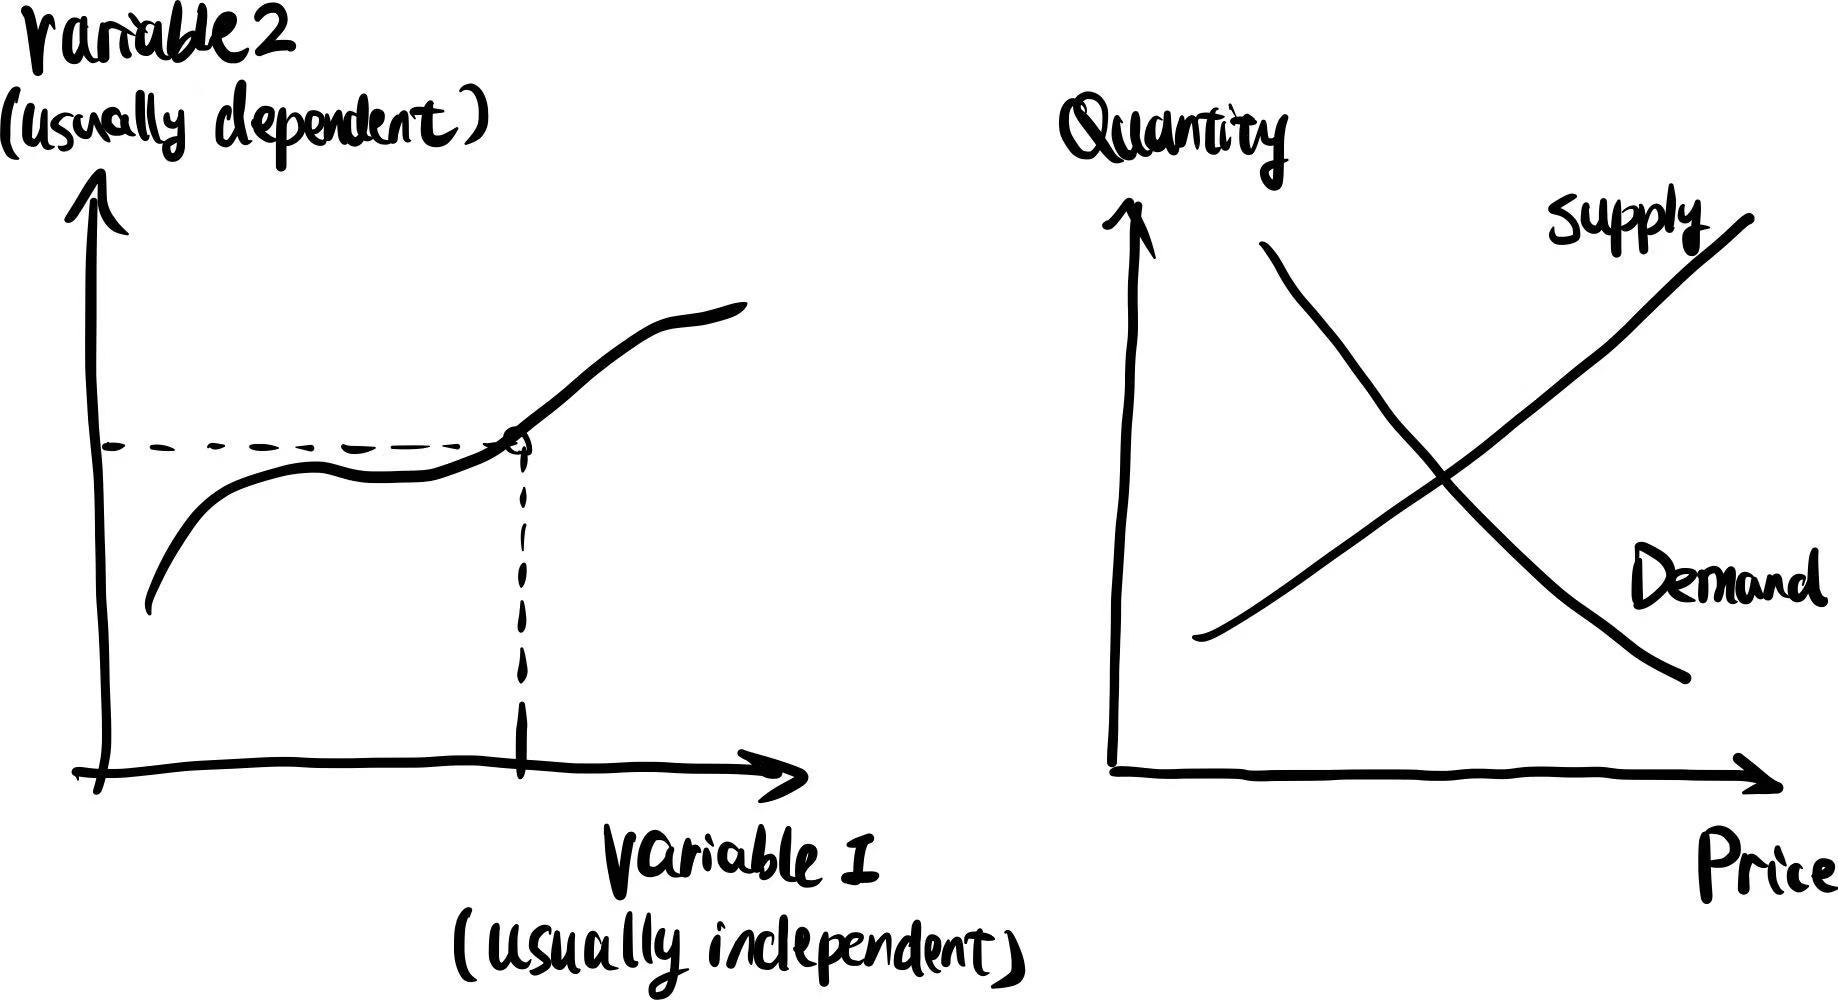
\includegraphics[width=0.9\textwidth]{img/image-20230228095149998.png}

\kaishu{\small 随着某商品的市场价格 (price) 增高, 生产者的生产意愿自然是增高的,
因为不考虑成本和其他因素变化的情况下 (Ceteris Paribus),
多生产的利润会更高, 因此供给曲线 (supply) 上扬, 反映出价格和供给量
(supply quantity) 的正相关; 另一方面,
消费者的消费意愿随着价格上涨自然是下降的, 于是需求曲线 (demand) 下压,
反映出价格和需求量 (demand quantity) 的负相关.

两条曲线分别对应着供给量和需求量关于价格的函数,
两函数的焦点反映了理想的自由市场下的最终成交价格和供需量
(因为在这个点达到了供需平衡 - equilibrium) ,
焦点向下作竖直线与横轴的焦点便显示了最终成交价格,
焦点向左作水平线与竖轴的交点便显示了平衡点的供需量.}
\end{tcolorbox}

在工程和计算机科学等思维里, 函数更像下左图所示, 给定一个输入 (input),
函数如同一台机器, 在加工后给出一个输出 (output); 这台机器非常可靠,
同样的输入能够稳定输出同样结果. 下右图给了一个例子

\begin{tcolorbox}[size=fbox, breakable, enhanced jigsaw]

\includegraphics[width=0.9\textwidth]{img/image-20230228095405809.png}

\kaishu{\small 假想有这样一个叫做``首都'' (Captital) 的函数,
放入一个国家名便会稳定输出这个国家的首都,
数学上我们可以这么标记下右图的例子 $\text{Capital(China)=Beijin}$.}
\end{tcolorbox}

函数的近现代定义和工科思维里的图景就很像, 考虑集合 $X$ 和 $Y$,
且它们不是空的, 如果存在某种特定的对应关系 $f$, 使得对于 $X$
中任意一个元素 $x$, 在 $Y$ 中都有唯一确定的元素 $y$ 和 $x$ 对应,
那么就称\textbf{映射} (mapping)\footnote{~Mapping 这个词用在这很贴切,
  map有地图的意思,
  ``映射''和地图上的每个点对应着实际区域上的一个个位置很相似.}
$f: A\rightarrow B$ 为从 $X$ 到 $Y$ 的一个函数, 记作
$y=f(x), x\in X$ 或者 $f(X)=\{y|f(x)=y, y\in Y\}$;
第一种记法强调元素的映射, 第二种记法强调整个集合的映射, $X$
在这里便是这个映射的定义域, $f(X)$ 是值域, $Y$
是这个映射的\textbf{陪域} (codomain, 也叫做上域, 到达域, 对应域),
大括号表示 $X$ 被映射到的集合, 其元素 $y$ 满足竖线后的条件, 即 $y$
是自 $x$ 通过 $f$ 这个映射得到, 并且 $y$ 属于 $Y$.
这样定义的直观感受类似下左图, 之前``首都''函数便类似下右图

\begin{tcolorbox}[size=fbox, breakable, enhanced jigsaw]
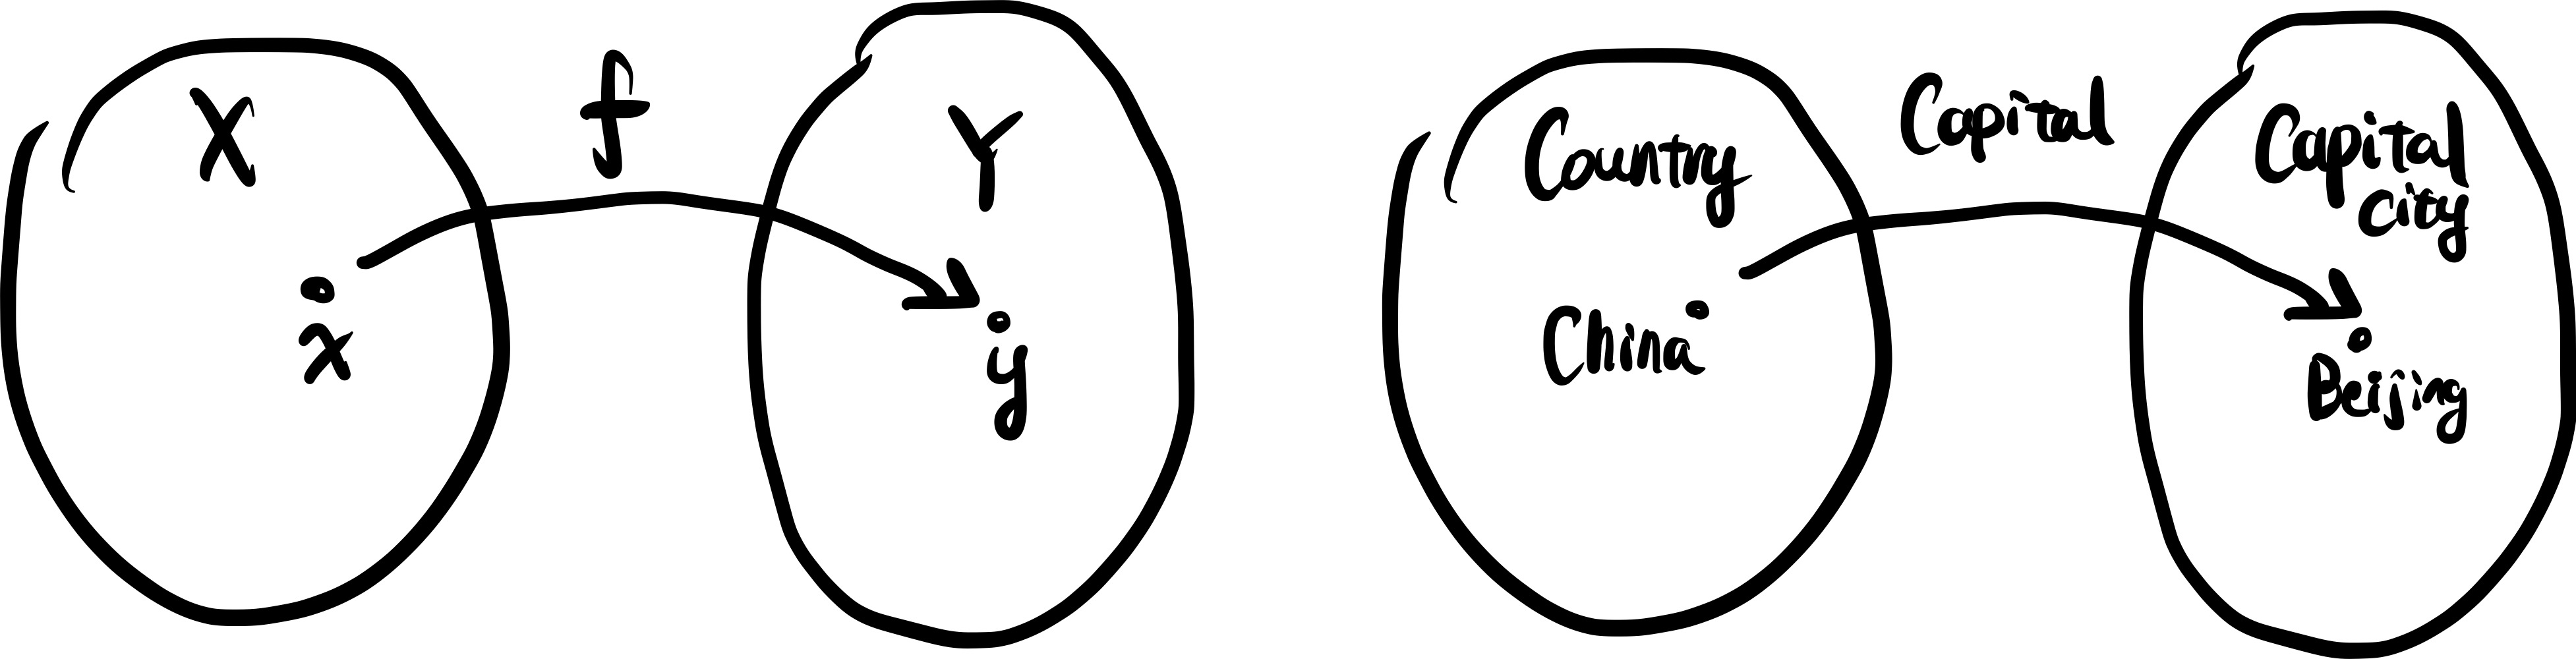
\includegraphics[width=0.9\textwidth]{img/image-20230228112941902.png}

\kaishu{\small Country这个集合里包含了很多国家, \{中国, 美国, 日本, \ldots\}; Capital
city这个集合里包含了很多城市, \{北京, 华盛顿, 东京, \ldots\};
Capital这个函数便描述了Country中的元素和Capital city中的元素的对应关系.}
\end{tcolorbox}

\end{tcolorbox}
\section{函数-下}\label{004}

\begin{flushright}{\kaishu 無名, 天地之始; 有名, 萬物之母. 常無, 欲以觀其妙; 常有, 欲以觀其徼. \\- 苏辙 『老子解』}\end{flushright}

\begin{tcolorbox}[size=fbox, breakable, enhanced jigsaw, title={单射, 满射, 双射 (injection, surjection,
bijection)}]

一个函数 $f:X\rightarrow Y$ 若满足, 如果 $a\neq b$ 则
$f(a)\neq f(b)$ 对于任何属于 $X$ 的 $a$ 和 $b$,
那么它便是\textbf{单射}的 (injection, one-to-one)\footnote{One-to-one
  是更``纯正''英语的说法, 比较通俗, injection 是来自法语的舶来词,
  更具高级感; 后面的 onto 和 surjection 同.}.

一个函数 $f:X\rightarrow Y$ , 若它的值域 (range) 和陪域 (codomain)
一致, 即对于任意 $y\in Y$, 都存在至少一个 $x\in X$ 满足
$f(x)=y$\footnote{介绍一下符号语言: $\exists$ - 存在; $\forall$ -
  对于所有. 于是这句话可以这么表述:
  $\forall y\in Y, \exists x\in X \text{ s.t. } f(x)=y$ (s.t.=such that
  可以译为``使得''). 但是通常情况下,
  还是尽量避免符号语言而使用自然语言来描述.}, 那么它便是\textbf{满射}的
(surjection, onto).

一个同时单射又满射的函数是\textbf{双射}的 (bijection, one-to-one
correspondance).

还是以Captial这个函数为例子, 下面给出了单射, 满射,
双射三种情况分别的图示:

\begin{tcolorbox}[size=fbox, breakable, enhanced jigsaw]
\begin{center}
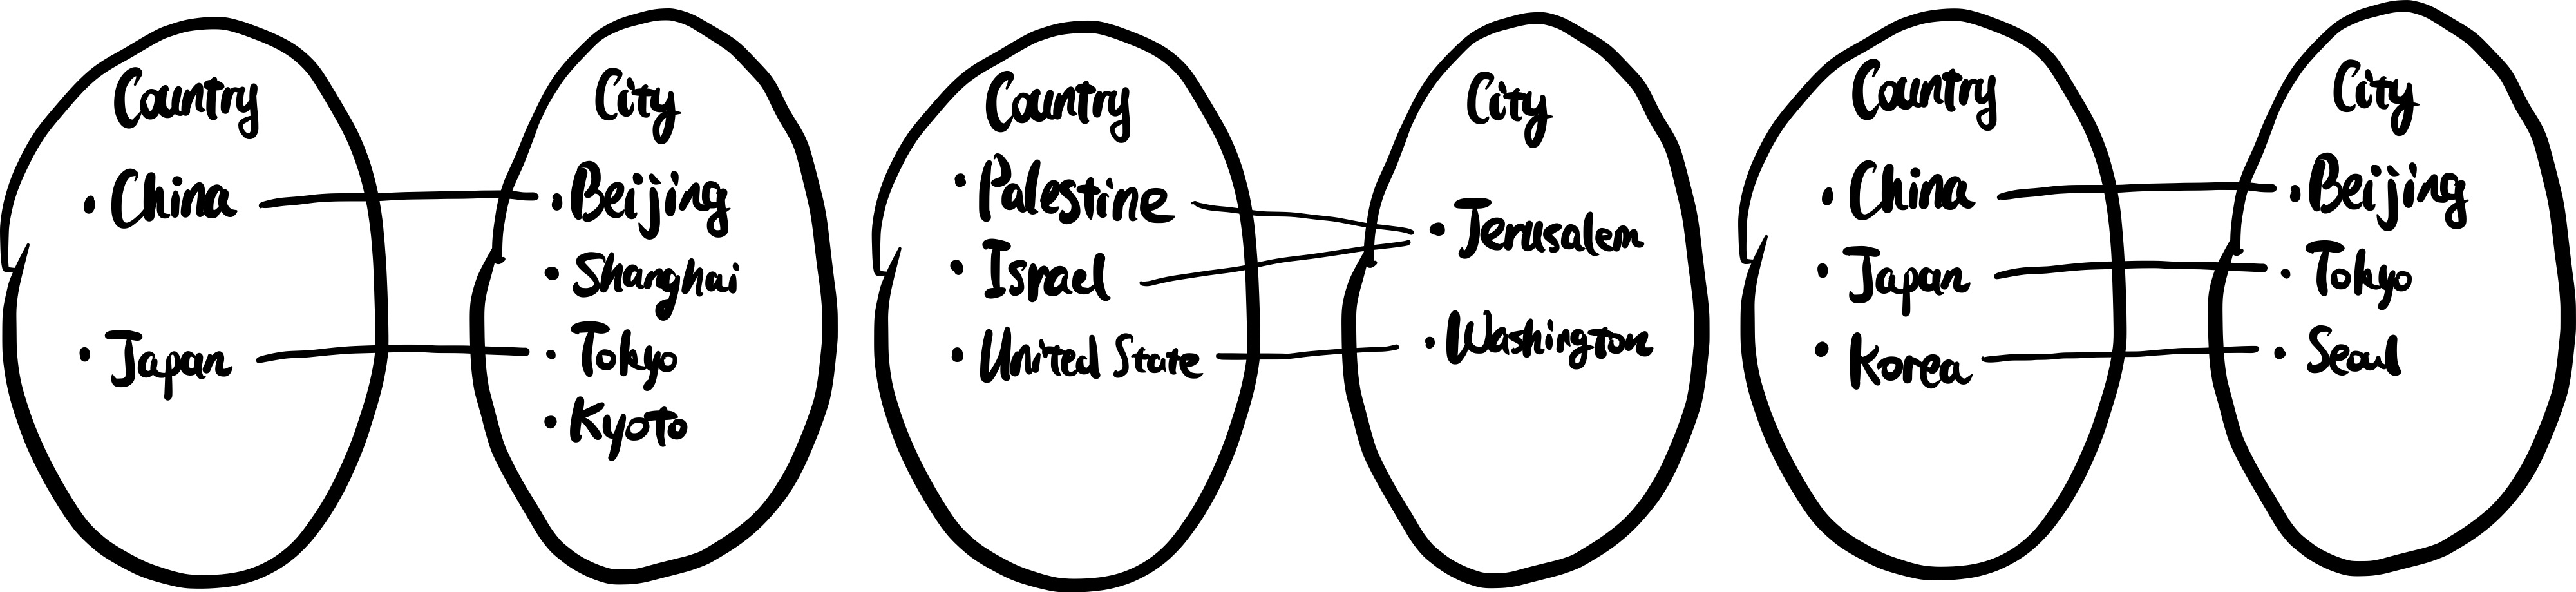
\includegraphics[width=0.9\textwidth]{img/image-20230302091706069.png}
\end{center}

\kaishu{\small 左: 单射但不满射; 中: 满射但不单射; 右: 双射.}
\end{tcolorbox}

\end{tcolorbox}

\begin{tcolorbox}[size=fbox, breakable, enhanced jigsaw, title={奇偶性 (parity 大嘘)}]

若一个函数满足 $f(-x)=-f(x)$, 即改变输入值 (自变量) 的正负号, 输出值
(因变量) 的正负号也改变, 这个函数便是\textbf{奇函数} (odd function).
图像上它是关于原点对称的.

若一个函数满足 $f(-x)=f(x)$, 即改变输入值 (自变量) 的正负号,
不影响输出值 (因变量) , 这个函数便是\textbf{偶函数} (even function).
图像上它是关于 $y$ 轴对称的.

当然, 奇函数和偶函数事实上是很特殊的两类函数,
更多的函数既不是奇函数又不是偶函数.

一些运算规律:

\begin{itemize}

\item
  奇函数 + 奇函数 = 奇函数\\{\kaishu 证明}: 假设存在两个奇函数 $f(x)$ 和
  $g(x)$, 令 $(f+g)(x) := f(x) + g(x)$, 即 $(f+g)(x)$
  这个函数是原本两函数之和. 根据奇函数的定义, $f(-x)=-f(x)$ 且
  $g(-x)=-g(x)$, 将两式相加得 $f(-x)+g(-x)=-f(x)-g(x)$, 即有
  $(f+x)(-x)=-(f+g)(x)$, 可见 $(f+g)(x)$ 是奇函数.
\item
  偶函数 + 偶函数 = 偶函数\\本条及接下来的证明与上一条类似, 可以当作练习.
\item
  奇函数 ×/÷ 奇函数 = 偶函数
\item
  偶函数 ×/÷ 偶函数 = 偶函数
\item
  奇函数 ×/÷ 偶函数 = 奇函数
\item
  偶函数 ×/÷ 奇函数 = 奇函数
\end{itemize}

\end{tcolorbox}

\begin{tcolorbox}[size=fbox, breakable, enhanced jigsaw, title={反函数 (inverse
function)}]

浅浅地非专业地叙述一下反函数. 设函数 $y=f(x)\ (x\in X)$ 的值域是
$Y$, 若存在一个函数 $g(y)$ 使得 $x= g(y)\ (y\in C)$, $g(x)$
便叫做 $f(x)$ 的\textbf{反函数} (inverse function), 可以记作
$x=f^{-1}(y)$, 它的定义域和值域分别是原函数的值域和定义域。

图像上, 反函数和原函数关于 $y=x$ 对称.

在求反函数时要特别注意反函数与原函数的定义域和值域. 例如 $y=f(x)=x^2$,
因为 $(\pm x)^2=y$, 反函数可能是 $x=f^{-1}(y)=\sqrt{y}$ 也可能是
$x=f^{-1}(y)=-\sqrt{y}$ , 但是不能是 $x=f^{-1}(y)=\pm\sqrt{y}$,
因为这样便不符合函数定义了, 一个输入值不可以有多个输出值,
或则说一个自变量不能对应多个因变量
(但是多个因变量对应一个自变量是允许的, 可以参考满射但不单射的图例).
这里反函数取正或负取决于原函数的定义域, 若 $y=f(x)=x^2, x\ge 0$, 则
$x=f^{-1}(y)=\sqrt{y}$; 若 $y=f(x)=x^2, x\le 0$, 则
$x=f^{-1}(y)=-\sqrt{y}$.

\end{tcolorbox}

\begin{tcolorbox}[size=fbox, breakable, enhanced jigsaw, title={隐函数 (implicit
function)}]

有的时候可能需要用函数来表达一个比较复杂的图像, 举一个简单一点的例子,
一个圆心位于原点的单位圆, 圆上任意一点到圆心距离都是 $1$, 于是有
$x^2+y^2=1$, 用前面学习的函数的形式表达这个关系, 有

$y=\begin{cases}\sqrt{1-x^2}\\-\sqrt{1-x^2}\end{cases}.$

这样似乎还没有起先的 $x^2+y^2=1$ 这个形式美观, 因此不妨还是用
$x^2+y^2-1=0$ 来表述单位圆上的 $x$ 与 $y$ 的关系. 类似这样,
利用一个【同时关于 $x$ 与 $y$ 的表达式 $F(x,y)=0$】来确定【 $y$
关于 $x$ 的函数】的表达式, 我们称之为\textbf{隐函数} (implicit
function); 为表区分, 前面介绍的类似 $y=f(x)$ 的函数,
称为\textbf{显函数} (explicit function).

\end{tcolorbox}

\begin{tcolorbox}[size=fbox, breakable, enhanced jigsaw, title={线性 (linearity)}]

这是一个很好的特性, 并不局限于函数, 仅对于函数来说的话,
若一个函数是线性的, 便有

$f(a+b)=f(a)+f(b),\ f(ax)=af(x).$

\end{tcolorbox}
\section{三角函数}\label{005}

\begin{flushright}{\kaishu 道可道, 非常道; 名可名, 非常名.}\end{flushright}

\begin{tcolorbox}[size=fbox, breakable, enhanced jigsaw, title={三角函数
(trigonometry)}]

三角函数最基本的使用应该是表示直角三角形的变长比. 如下图所示, 三角形
$ABC$ 为直角三角形, 将 $\angle BAC$ 记作 $\theta$, 对于两条直角边
$AB$ 和 $BC$, 边 $AB$ 在 $\theta$ 边上, 称它为\textbf{邻边}
(adjacent), 边 $BC$ 在 $\theta$ 对面, 称它为\textbf{对边}
(opposite), 剩余的边 $AC$ 被称为\textbf{斜边} (hypotenuse)。

\begin{tcolorbox}[size=fbox, breakable, enhanced jigsaw]
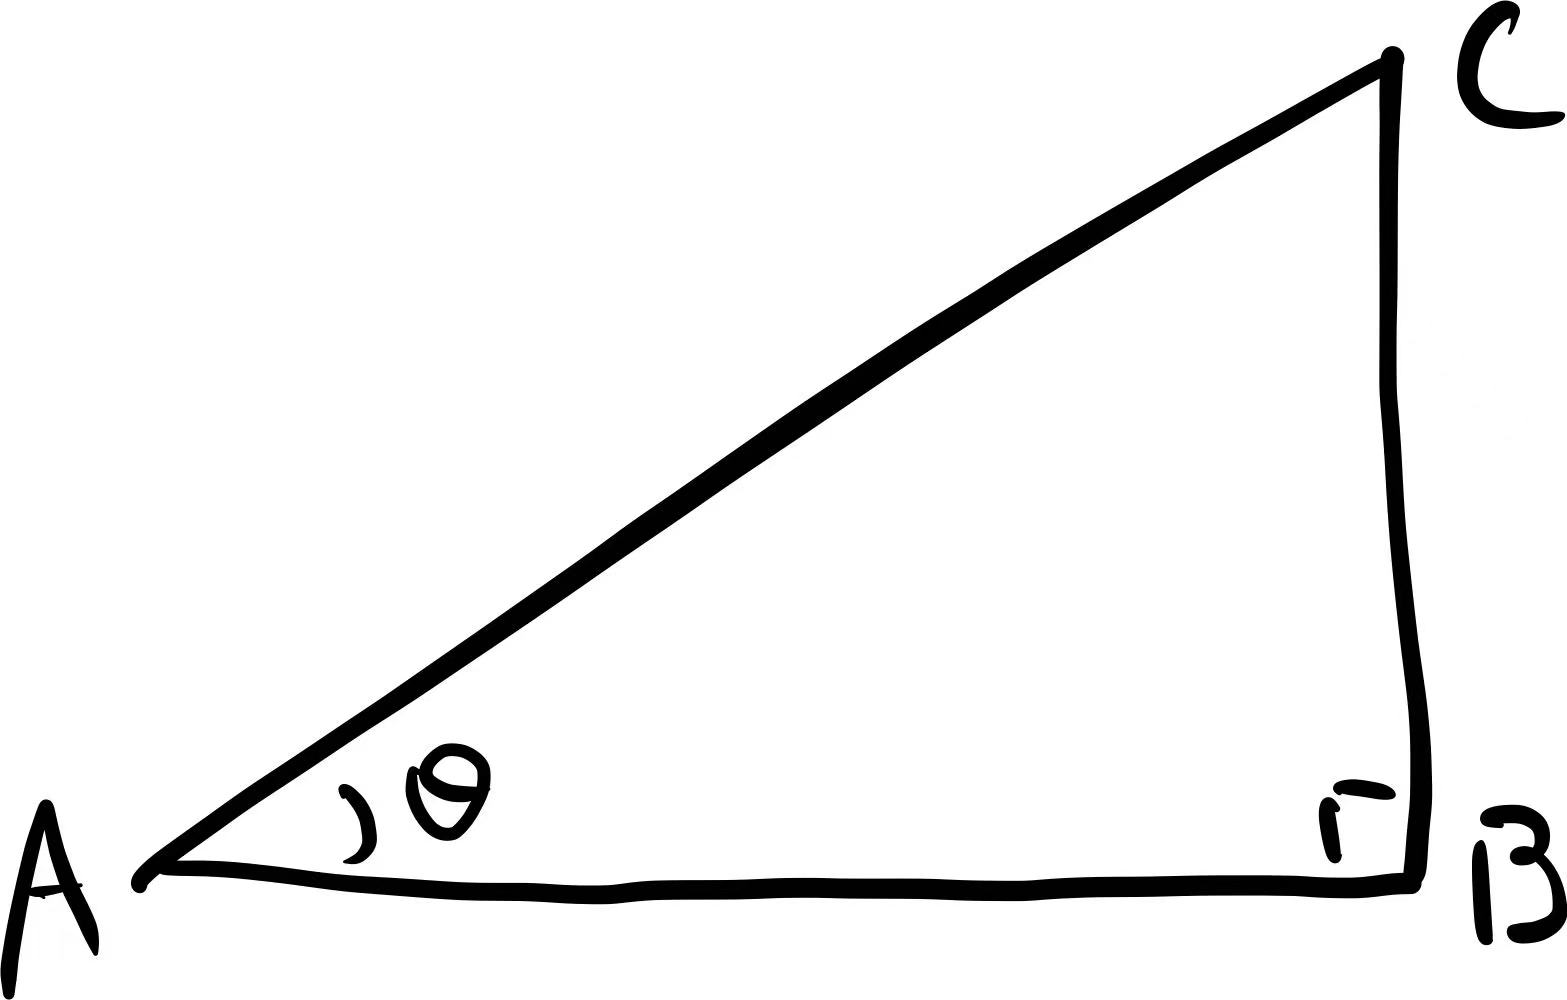
\includegraphics[width=0.5\textwidth]{img/image-20230308142717670.png}
\end{tcolorbox}

易见, 各变长比仅和 $\theta$ 相关\footnote{当然也可以说和除了直角外的另一个角
  $(90^\circ-\theta)$ 相关; 边长比可以通过一个除直角外的角确定是因为,
  除直角外另一角相等的直角三角形都相似, 它们的边长比是一致的。},
三角函数便是用来表示各个比例的, 常用的三角函数有

$\begin{aligned}\cos\theta&=\frac{\text{邻边}}{\text{斜边}}=\frac{AB}{AC},\\ \sin\theta&=\frac{\text{对边}}{\text{斜边}}=\frac{BC}{AC},\\ \tan\theta&=\frac{\text{对边}}{\text{邻边}}=\frac{BC}{AB}.\end{aligned}$

不难看出$\tan\theta=\frac{\sin\theta}{\cos\theta}$.

另外还有

$\begin{aligned}\sec\theta&\equiv\frac{1}{\sin\theta},\\ \csc\theta&\equiv\frac{1}{\cos\theta},\\ \cot\theta&\equiv\frac{1}{\tan\theta}.\end{aligned}$

$\csc$ 很多时候也记作 $\text{cosec}$.

一个非常实用的关系, 直角三角形中有\textbf{勾股定理} (Pythagorean
theorem): 斜边边长平方等于两直角边边长的平方之和, 即 $AC^2=AB^2+BC^2$;
两边同时除以 $AC^2$ 便有

\begin{itemize}

\item
  $\boxed{1=\cos^2\theta+\sin^2\theta}$.\footnote{三角函数的平方:
    cos(x)\textsuperscript{2} 通常理解为 cos((x)\textsuperscript{2});
    cos\textsuperscript{2}x 约定俗成表示 (cos(x))\textsuperscript{2}.}
\end{itemize}

\end{tcolorbox}

\begin{tcolorbox}[size=fbox, breakable, enhanced jigsaw, title={反三角函数}]

三角函数, 输入一个角度, 返回一个边长比; 反三角函数便是三角函数得逆运算,
或者说反函数 (参见【\ref{004}\nameref{004}】), 即输入一个边长比, 返回一个角度.

\end{tcolorbox}

\begin{tcolorbox}[size=fbox, breakable, enhanced jigsaw, title={正弦定律 (law of sine)}]

将三角形三个角分别记作 $\alpha$, $\beta$, 和 $\gamma$,
将它们的对边分别记作 $A$, $B$, 和 $C$. 先是结论:

\begin{itemize}

\item
  $\boxed{\frac{A}{\sin\alpha}=\frac{B}{\sin\beta}=\frac{C}{\sin\gamma}}$.
\end{itemize}

\begin{tcolorbox}[size=fbox, breakable, enhanced jigsaw]
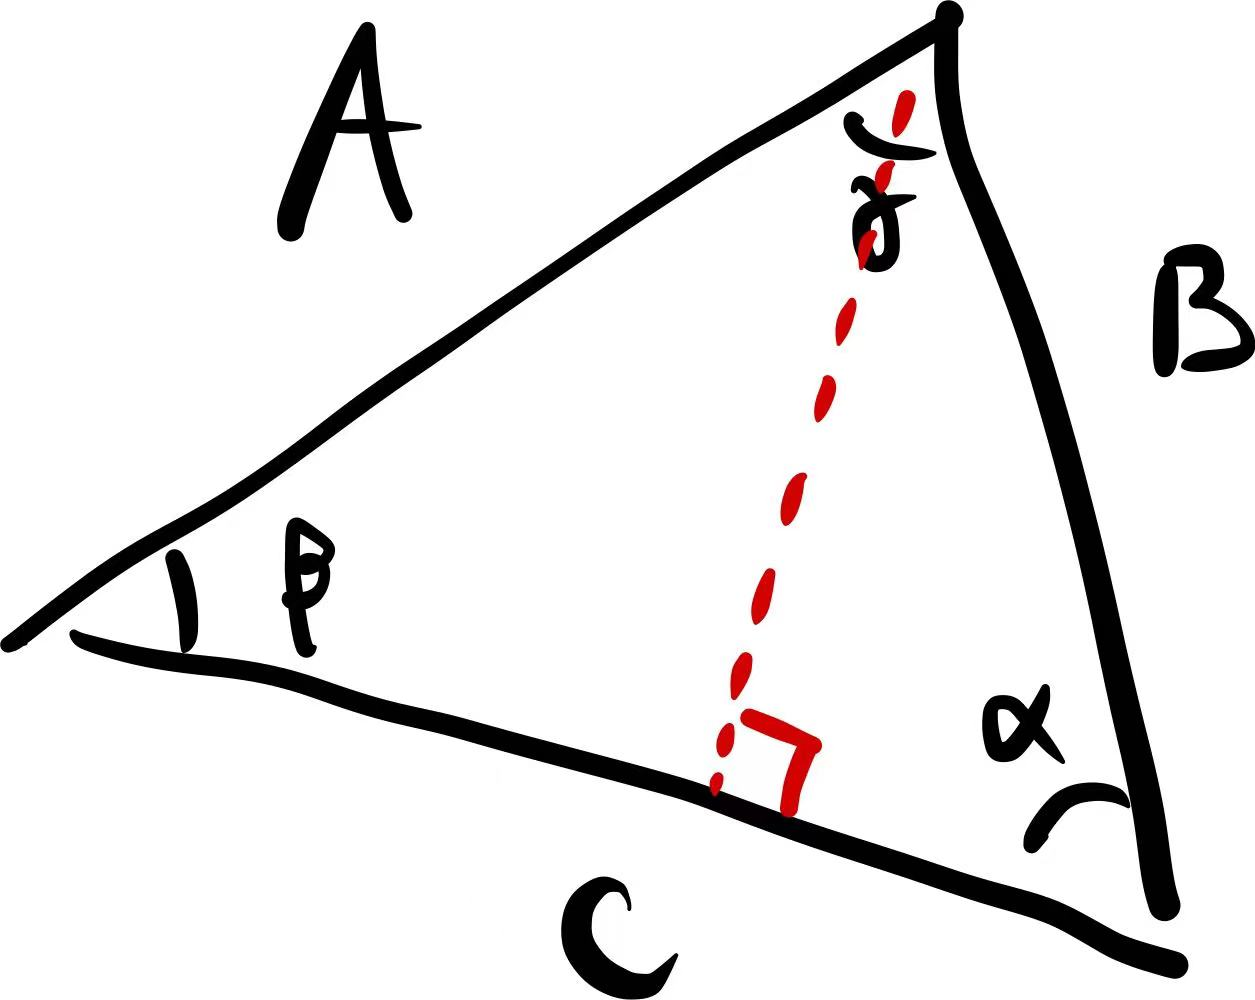
\includegraphics[width=0.5\textwidth]{img/image-20230308142913522.png}
\end{tcolorbox}

推导如下:

如上图所示, 以 $C$ 为底做高, 将原本的三角形分为左右两个直角三角形,
这条高利用左边的直角三角形可以表示为 $A\sin\beta$,
利用右边的直角三角形则是 $B\sin\alpha$, 于是有
$A\sin\beta=B\sin\alpha$, 整理可得
$\frac{A}{\sin\alpha}=\frac{B}{\sin\beta}$;
再做另一条高重复前面的操作, 便可得到完整的结论.

\end{tcolorbox}

\begin{tcolorbox}[size=fbox, breakable, enhanced jigsaw, title={余弦定律 (law of cosine)}]

还是先上结论:

\begin{itemize}

\item
  $\boxed{B^2=A^2+C^2-2AC\cos\beta}$,
\end{itemize}

即, 【一条边的边长平方】等于【另两条边的边长平方之】和加上【两倍的
(另两条边边长的乘积) 乘以 (另两条边的夹角的余弦)】.

\begin{tcolorbox}[size=fbox, breakable, enhanced jigsaw]
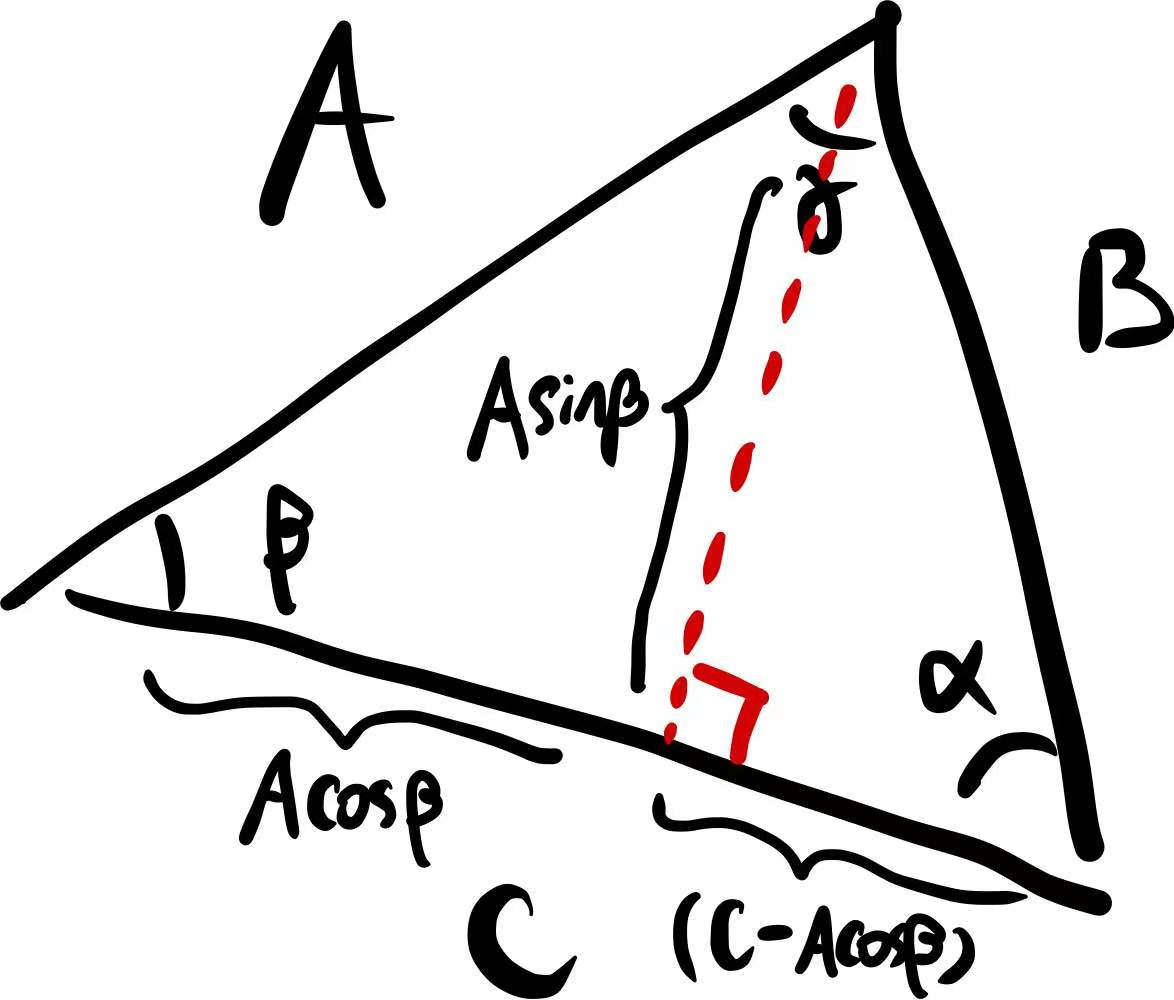
\includegraphics[width=0.5\textwidth]{img/image-20230308151417631.png}
\end{tcolorbox}

推导如下:

如下图所示, 依旧利用底边 $C$ 上的高将其分为左右两个直角三角形;
左边的直角三角形, 利用斜边 $A$ 和角 $\beta$, 两直角边分别可以表示为
$A\cos\beta$ 和 $A\sin\beta$, 于是右边的直角三角形边长便可表述为
$A\sin\beta$ 和 $(C-A\cos\beta)$; 对右边的直角三角形使用勾股定理

$\begin{aligned}B^2&=A^2\sin^2\beta+(C-A\cos\beta)^2\\ &=A^2\sin^2\beta+C^2+A^2\cos^2\beta-2AC\cos\beta\\ &=A^2+C^2-2AC\cos\beta.\end{aligned}$

其中等式的后两行用到了之前得出的 $1=\cos^2\theta+\sin^2\theta$.

\end{tcolorbox}

\begin{tcolorbox}[size=fbox, breakable, enhanced jigsaw, title={任意角度的三角函数}]

不难发现, 前面讨论的情况似乎都是锐角的情况 (主要是因为插图\ldots),
钝角的三角函数似乎没那么直观了, 因为做不成一个含有钝角的直角三角形,
没法简单地用边长比来表示 $\sin$ 和 $\cos$ 等. 于是,
我们需要想办法将前面的情形推广.

如下左图所示, 建立直角坐标系, 做一圆心位于原点的单位圆, 即半径为 $1$
的圆, 考虑在第一象限的圆上的一点, 将其与原点做连线, 将从
$x$-轴正方向与这条连线\textbf{顺时针}方向形成的夹角记作 $\theta$,
不难看出这个点的坐标 $(x,y)$ 满足

$\begin{cases}x=\cos\theta,\\y=\sin\theta.\end{cases}$

\begin{tcolorbox}[size=fbox, breakable, enhanced jigsaw]
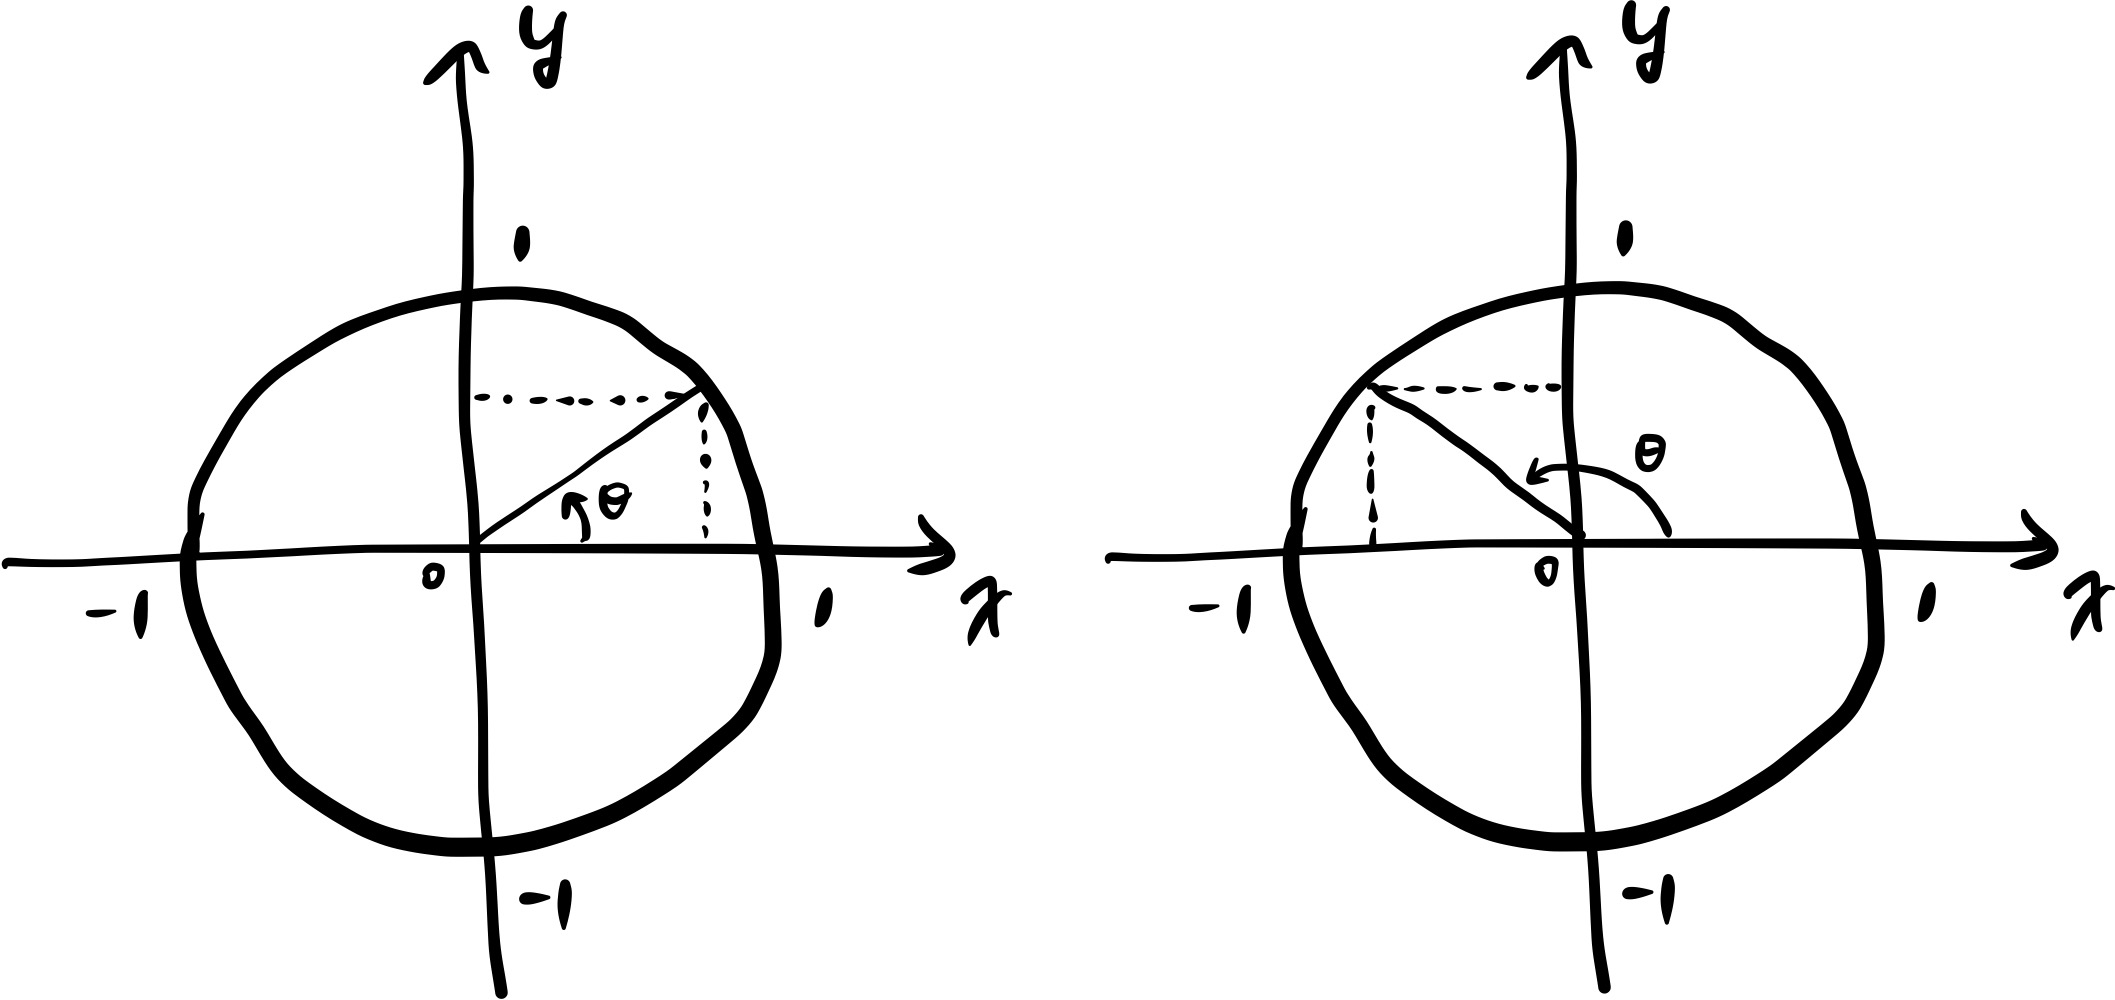
\includegraphics[width=0.75\textwidth]{img/image-20230316171124433.png}
\end{tcolorbox}

于是不妨将其他象限的情况也按此定义,
于是如上右图所示的钝角甚至更大角度的三角函数便可以被定义了.

\end{tcolorbox}

\begin{tcolorbox}[size=fbox, breakable, enhanced jigsaw, title={弧度制 (radian)}]

为什么一个周角是 $360^\circ$ 呢, 听说过一个不可考的说法: $360$
是一个有很多因数的数字 (1, 2, 3, 4, 5, 6, 8, 9, 10, 12\ldots),
等分起来的时候数字会比较友好, 所以 $360^\circ$ 其实是非常随意地规定的.
那么有没有更好的用来描述角度方法呢? 答案是弧度.

一个半径为 $r$ 的圆的周长是 $2\pi r$, 一个圆心角为 $n^\circ$
的扇形的弧长是 $2\pi r\frac{n}{360}$. 可见圆心角越大弧越长,
且圆心角和弧长成正比. 既然如此,
不如重新将角度定义为圆心角与弧长的比值以方便计算, 于是便有了,
在新的这套单位系统中, 若圆心角大小为 $\theta$, 其对应弧长应为
$r\theta$; 当圆心角是一个周角时, 对应弧长便成了圆的周长 $r(2\pi)$.
所以角度和这个新的单位的换算有 $360^\circ\equiv 2\pi\ \text{rad}$,
因为这个单位把圆心角和对应的弧长联系起来了, 因此称之为\textbf{弧度}
(radian).

扇形面积在这套单位制, 即弧度制下, 便也成了 $\frac{1}{2}r^2\theta$.

\end{tcolorbox}

\begin{tcolorbox}[size=fbox, breakable, enhanced jigsaw, title={三角函数的图像}]

现在这个时代, 大家都或多或少能接触到科学计算器,
再不济在bing.com上搜索``solver''用微软的 Microsoft Solver
也可以计算某个特定角度的三角函数值, 自然也可以绘制函数图像.
下图分别展示了 $\sin(x)$ 和 $\cos(x)$ 的图像,

\begin{tcolorbox}[size=fbox, breakable, enhanced jigsaw]
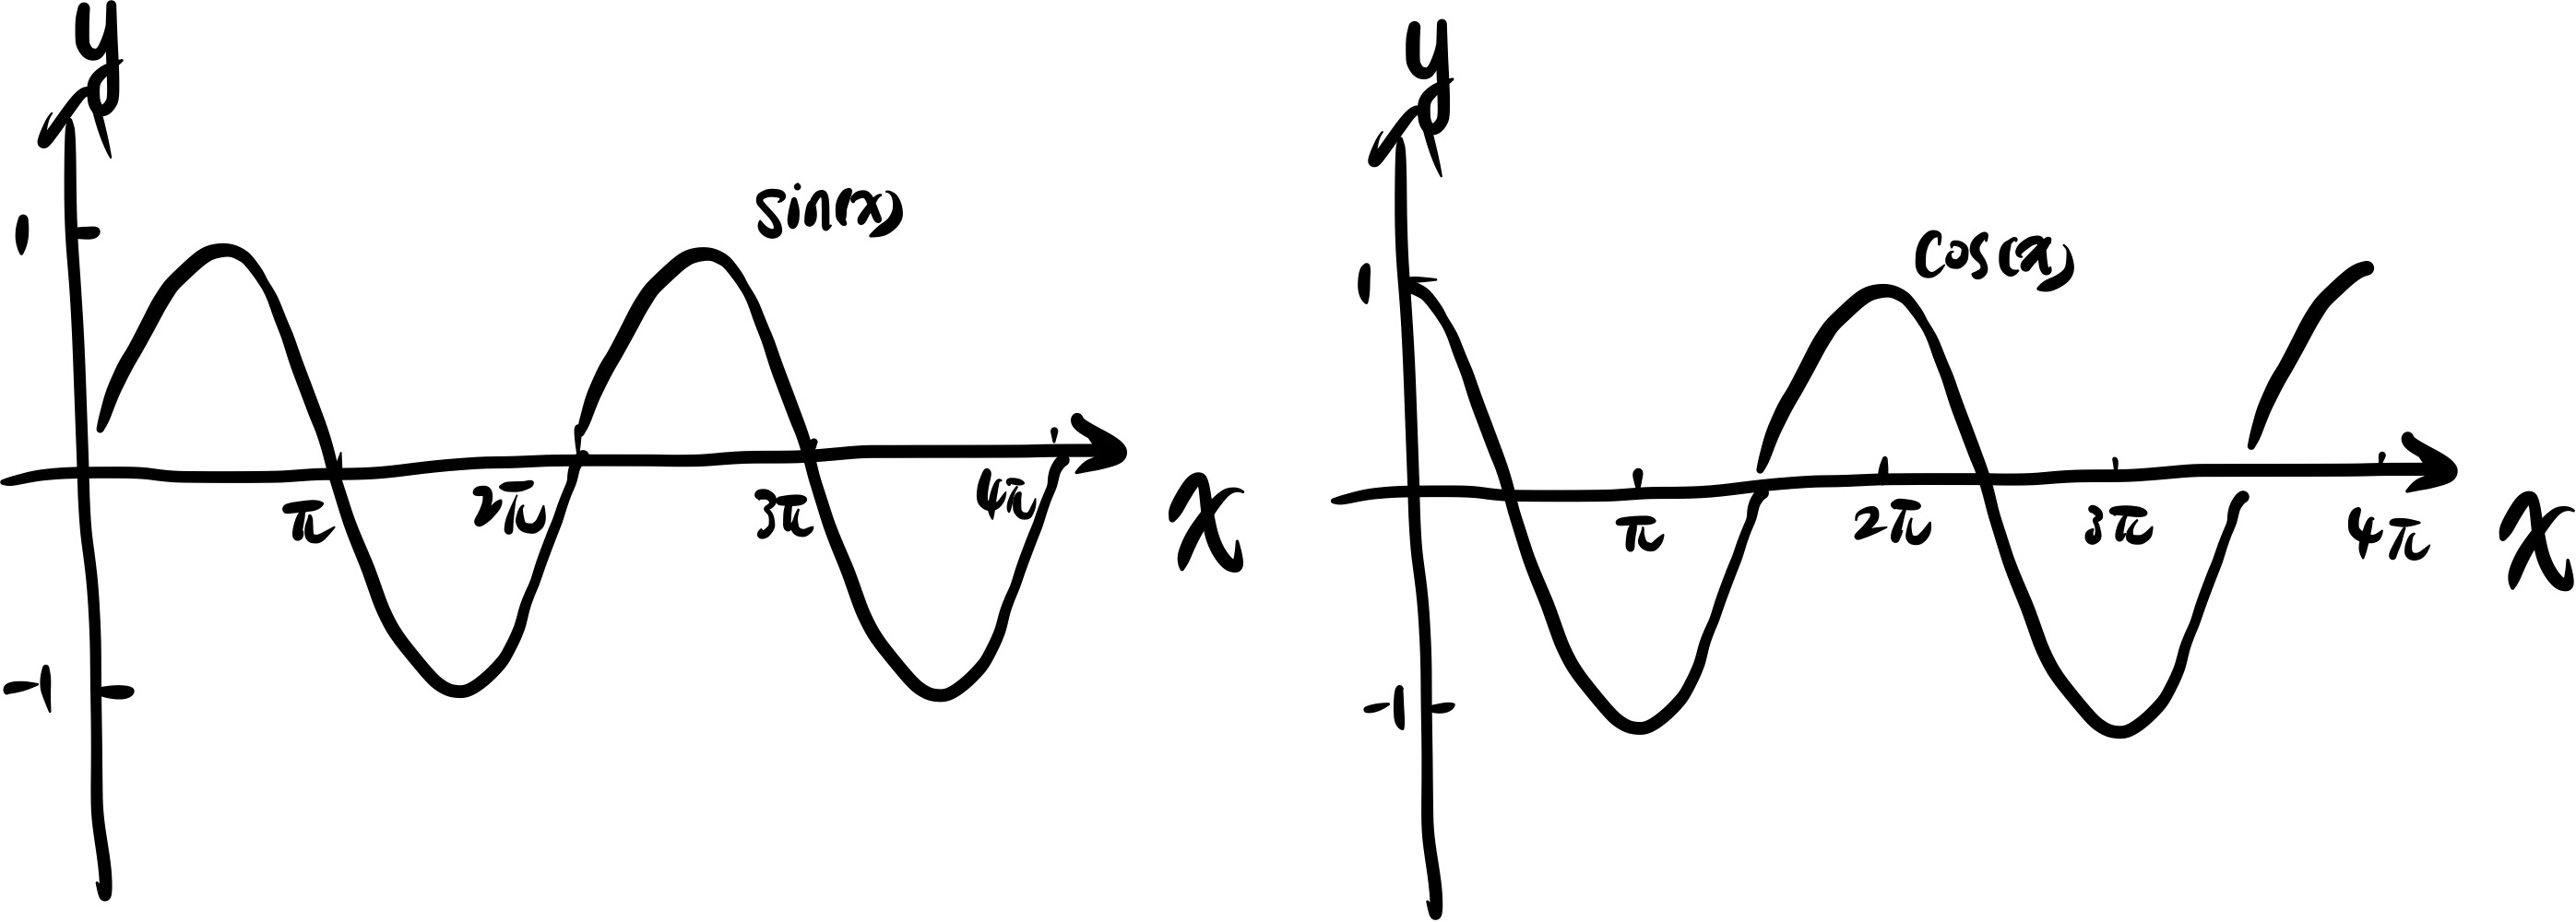
\includegraphics[width=0.75\textwidth]{img/image-20230316171137500.png}
\end{tcolorbox}

一些值得关注的点是它们都是\textbf{周期函数} (periodic function),
随着自变量-角度的变化, 因变量-函数值的变化是周期性的, 它们的周期都是
$2\pi$, 这一点从上文的单位圆里便可看出些许原因,
当角度变化超过一个周角时, 和角度刚从 $0$ 开始的情况是一样的.

\end{tcolorbox}
\section{虚数和复数}\label{006}

\begin{flushright}{\kaishu 些许绕行 (detour).}\end{flushright}

\begin{tcolorbox}[size=fbox, breakable, enhanced jigsaw, title={虚数和复数 (imaginary number and complex number)}]

考虑一个一元二次方程 $ax^2+bx+c=0$, 它的解有

$\begin{aligned}
0&=a\left(x^2+\frac{b}{a}x+\frac{c}{a}\right)\\
0&=x^2+\frac{b}{a}x+\frac{c}{a}\\
0&=x^2+\frac{b}{a}x+\left(\frac{b}{2a}\right)^2-\left(\frac{b}{2a}\right)^2+\frac{c}{a}\\
0&=\left(x-\frac{b}{2a}\right)^2-\left(\frac{b}{2a}\right)^2+\frac{c}{a}\\
\left(x-\frac{b}{2a}\right)^2&=\left(\frac{b}{2a}\right)^2-\frac{c}{a}\\
&...\\
x&=\boxed{\frac{-b\pm\sqrt{b^2-4ac}}{2a}}.
\end{aligned}$

上式最后的结论便是求根公式, 不难看出整个推导过程实际上就是配方,
其中根号前面的``加减''是因为对等式两边同时开方时,
正负两种情况都是正确的.

我们在此之前接触到的数字都还限于实数范围内, 因此会要求
$\left(b^2-4ac\right)$ 是正的, 以保证开方之后的结果是``有意义的'',
然而

\begin{newquote}
    ``从来如此, 便对么?''
\end{newquote}

之前也出现了, 不能被表示成分数形式的数字,
我们的研究范围从有理数扩充到了实数; 现在, 若 $\left(b^2-4ac\right)$
是负的, 按照当前的理解, 它不能被开方, 那是不是又到了这样一个神圣的时刻,
我们需要拓展我们研究的数字的范围?

既然如此, 不如规定 $\sqrt{-1}\equiv i$, 作为新的一类数字的单位,
因为之前的数字叫``实数'', 那么这一类新的数字就不妨叫做``\textbf{虚数}''
(imaginary number) 吧. 一个既包含实数部分, 又包含虚数的部分的数字,
我们就叫它``\textbf{复数}'' (complex number), 记作 $\mathbb{C}$.
\end{tcolorbox}

\begin{tcolorbox}[size=fbox, breakable, enhanced jigsaw, title={运算规律}]

考虑若干个复数, $z_1=a+bi$, $z_2=c+di$, $z_3=e+fi$\ldots{}

\begin{itemize}

\item
  \textbf{加法}: $z_1+z_2=(a+c)+(b+d)i$.
  实数部分和虚数部分可以分开计算,
  应该不难看出复数和加法是构成\textbf{阿贝尔群}的
  (即它具有封闭性和结合律, 有单位元和逆元, 并且有交换律, 详细参见\ref{001}\nameref{001}).
\item
  \textbf{乘法}:
  $z_1\times z_2=(a+bi)\times(c+di)\\=ac+adi+bci+bdi^2=(ac-bd)+(ad+bc)i.$
  不难看出, 复数和乘法也构成阿贝尔群.
\item
  乘法对于加法满足\textbf{分配律}, 即,
  $(z_1+z_2)\times z_3=z_1\times z_3+z_2\times z_3$,
  证明留作练习\footnote{事实上, 很多情况下, 之前提到的很多知识点,
    例如单位元, 零元, 逆元都分左右, 分配律也有左分配律和右分配律,
    但是目前讨论的情况都是满足交换律的, 所以可以不区分左右.}.
\end{itemize}

以上三条已经足够使得复数与加法和乘法构成一个\textbf{环} (ring), 事实上,
环只需要乘法是半群 (semi-group, 即满足结合律和有单位元的二元运算与集合) 即可.

\begin{itemize}

\item
  \textbf{减法}: 因为加法存在逆元, 所以减去一个数,
  可以视作加上这个数的加法逆元, 即:
  $z_1-z_2=(a+bi)-(c+di)\\\Rightarrow z_1+(-z_1)=(a+bi)+(-(c+di))=(a-c)+(b-d)i$
\item
  \textbf{除法}: 不难发现每个非零的元素都有乘法逆元,
  因此除以一个数可以视作乘上这个数的乘法逆元, 即: 因为
  $z_2\times\frac{1}{z_2}=\frac{c+di}{c+di}=1$, 于是
  $z_1\div z_2=z_1\times\frac{1}{z_2}=\frac{a+bi}{c+di}$.
\end{itemize}

\begin{newquote}
一点小插曲, $\frac{a+bi}{c+di}$ 应该怎么化简呢,
怎么写成简单的实数部分加上虚数部分的形式呢?
回顾一下无理数的``分母有理化'', 例如有
$\frac{a+\sqrt{b}}{c+\sqrt{d}}$, 我们会将分子分母同时乘以
$(c-\sqrt{d})$ 将分母变为有理数, 便有
$\frac{(a+\sqrt{b})(c-\sqrt{d})}{c^2-d}$. 类似的, 当我们尝试化简
$\frac{a+bi}{c+di}$时, 我们也不妨对分子分母同时乘以 $(c-di)$, 于是有
$\frac{(a+bi)(c-di)}{c^2+d^2}$, 分母便变为了实数,
再稍加化简便可转化为一个实数加上一个虚数的形式. 我们称 $(c-di)$ 是
$(c+di)$ 的\textbf{复共轭} (complex conjugate)\footnote{两头牛背上的架子称为轭,
  轭使两头牛同步行走. 共轭就描述了两个对象这样一种相生相随的关系.}.
\end{newquote}

像上述这样可以进行加减乘和除零外除法,
并满具足一些特定的阿贝尔群的特点和分配律的代数结构,
换言之一个满足交换律的环 (交换环 commutative ring)
附加上除零外元素的除法运算, 构成一个\textbf{域} (field), 可以记作
$\mathbb{F}$, 常见的例子有有理数域, 实数域, 复数域.

\begin{tcolorbox}[size=fbox, breakable, enhanced jigsaw]
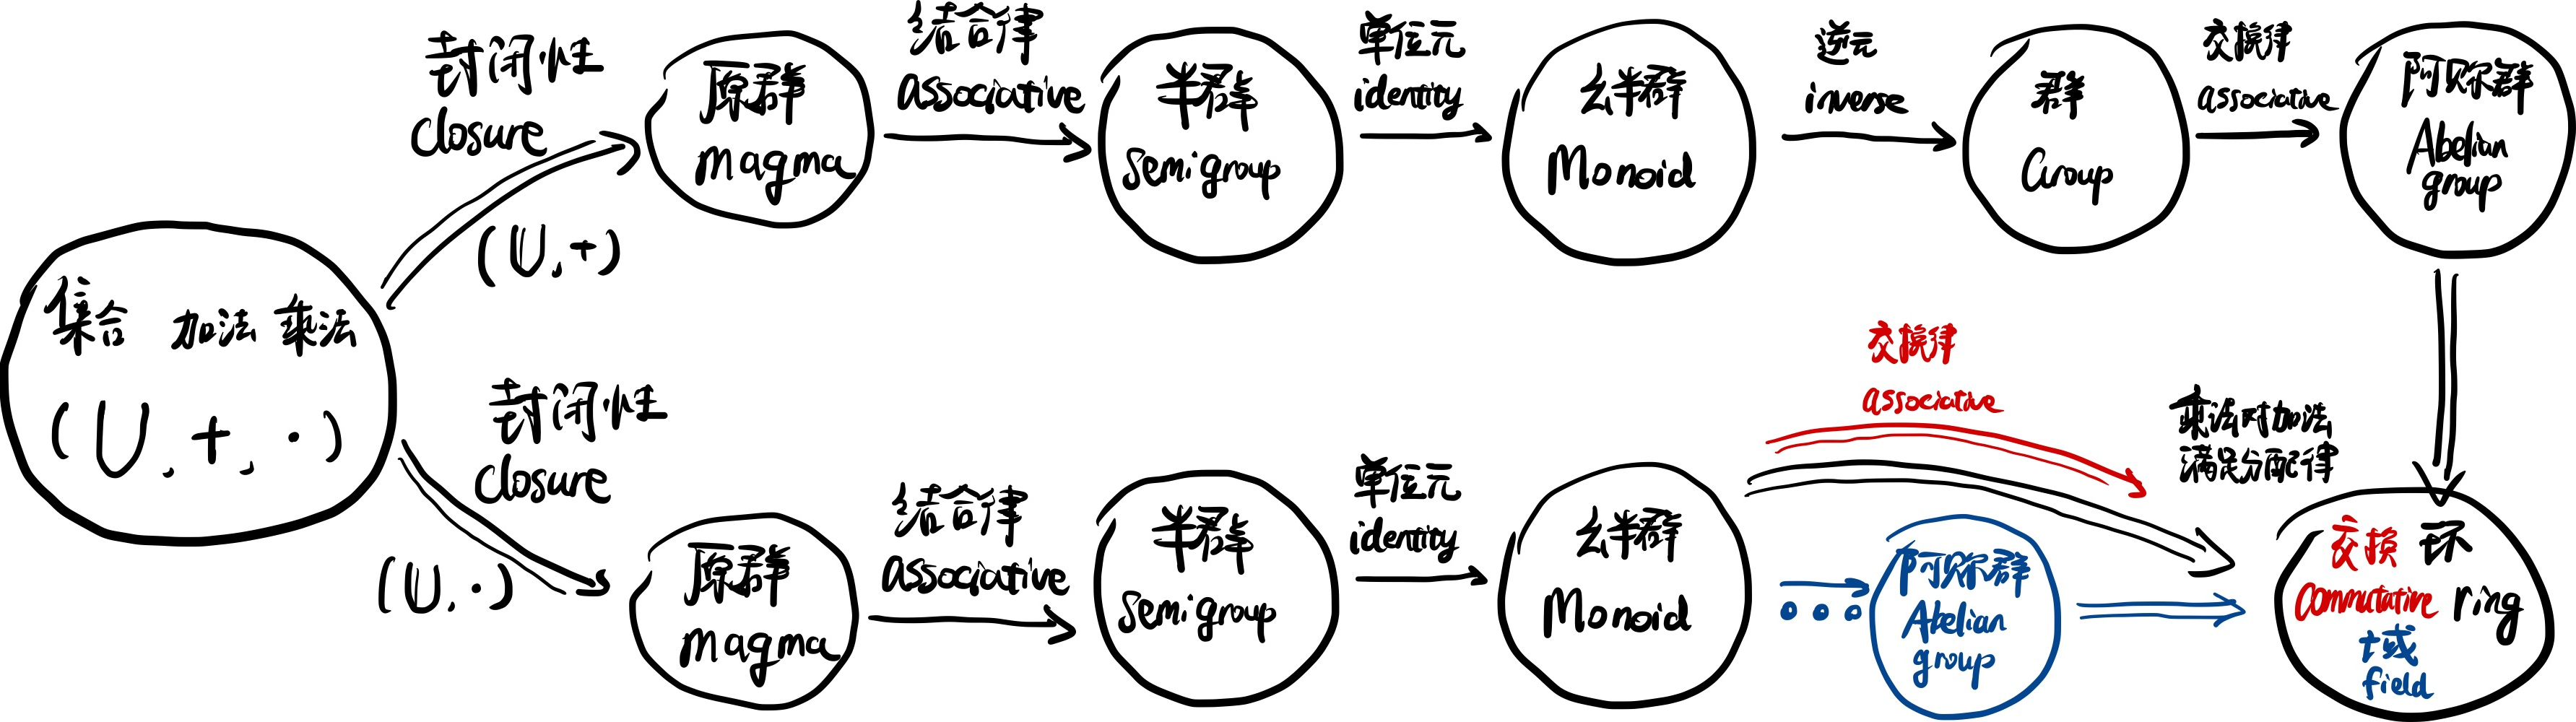
\includegraphics[width=0.9\textwidth]{img/image-20230328100716650.png}

\kaishu{\small 环, 交换环, 域的关系, 图改自知乎@SparkAndShine}
\end{tcolorbox}

\end{tcolorbox}
\begin{quote}
绕行之绕行 (detour of the detour).
\end{quote}

\hypertarget{ux4e8cux9879ux5f0fux5c55ux5f00-binomial-expansion}{%
\subsubsection{二项式展开 (binomial
expansion)}\label{ux4e8cux9879ux5f0fux5c55ux5f00-binomial-expansion}}

\textbf{二项式展开}指的是将类似 \((x+y)^n\) 的表达式展开的过程. 结论上有

\(\boxed{(x+y)^n=\sum_{r=0}^n\binom{n}{r}x^{n-r}y^r}.\)

这里 \(\binom{n}{r}=\frac{n!}{r!(n-r)!}\) 也记作 \(_nC_r\),
这个''C''是\textbf{组合} (combination) 的意思, 其中又有
\(n!=n\times(n-1)\times...\times3\times2\times1\).

\begin{quote}
上面第一次出现了求和符号 \(\sum\), 在此用一些例子说明,

\(\sum_{i=1}^{10}i=1+2+3+...+9+10;\)

\(\sum_{x=1}^{10}x^2=\left.x^2\right|_{x=1}+\left.x^2\right|_{x=2}+...+\left.x^2\right|_{x=10}=1^2+2^2+...+10^2.\)

即, 求和符号后的表达式, 依次代入求和符号下方的值,
符号下方的值加一\ldots, 直至代入求和符号上方的值, 最后将这些项求和.
\end{quote}

二项式展开的证明思路如下:

\textbf{从组合的思路出发}

\begin{itemize}
\item
  将 \((x+y)^n=\underbrace{(x+y)(x+y)...(x+y)}_{n}\) 展开,
  并将同类项合并, 易见可能出现的项的形式仅为 \(x^n=x^ny^0\),
  \(x^{n-1}y=x^{n-1}y^1\), \(x^{n-2}y^2\), \ldots{} \(x^2y^{n-2}\),
  \(xy^{n-1}=x^1y^{n-1}\), \(y^n=x^0y^n\).
\item
  合并后这些项的系数是合并前它们分别出现的次数,

  \begin{itemize}
  \tightlist
  \item
    \(x^n\) 相当于展开时每一个 \((x+y)\) 都选取 \(x\) 的情况,
    只有一种这样的情况, 即合并前 \(x^n\) 只可能出现 \(1\) 次,
    那么合并后它的系数便是 \(1\).
  \item
    \((x^{n-1}y^1)\) 相当于展开时每一个 \((x+y)\) 选取了 \((n-1)\) 个
    \(x\) 和 \(1\) 个 \(y\), 利用组合学的知识有
    \(n=\frac{n!}{1!(n-1)!}\) 种这样的情况, 即合并前 \((x^{n-1}y^1)\)
    出现 \(n\) 次, 那么合并后它的系数便是 \(n\).
  \end{itemize}

  \begin{quote}
  这个 \(n\) 可以这么看待, 选取的这个 \(y\) 可以出自这 \(n\) 项
  \((x+y)\) 中的任意一个, 于是便有 \(n\) 种可能.
  \end{quote}

  \begin{itemize}
  \tightlist
  \item
    \((x^{n-2}y^2)\) 相当于展开时每一个 \((x+y)\) 选取了 \((n-2)\) 个
    \(x\) 和 \(2\) 个 \(y\), 利用组合学的知识有
    \(\frac{n(n-1)}{2!}=\frac{n!}{1!(n-1)!}\) 种这样的情况, 即合并前
    \((x^{n-1}y^1)\) 出现 \(n\) 次, 那么合并后它的系数便是 \(n\).
  \end{itemize}

  \begin{quote}
  这个 \(\frac{n(n-1)}{2!}\) 可以这么看待, 选取的这两个 \(y\) 可以出自这
  \(n\) 项 \((x+y)\) 中的任意两个, 第一个 \(y\) 有 \(n\) 种选法,
  第二个因为第一个''占用''了一个 \((x+y)\), 因此它只有 \((n-1)\) 种选法,
  综上便有了 \(n(n-1)\); 然后两个 \(y\) 的顺序是无所谓的, 两个 \(y\)
  本身先后的排序会额外引入一个倍数 \(2\), 于是除掉.
  \end{quote}

  \begin{itemize}
  \tightlist
  \item
    \ldots{}
  \item
    \((x^{n-r}y^r)\) 相当于展开时每一个 \((x+y)\) 选取了 \((n-r)\) 个
    \(x\) 和 \(r\) 个 \(y\), 利用组合学的知识有
    \(\frac{n(n-1)...(n-r)}{(n-r)!}=\frac{n!/r!}{(n-r)!}=\frac{n!}{1!(n-1)!}=\binom{n}{r}\)
    种这样的情况, 即合并前 \((x^{n-1}y^1)\) 出现 \(\binom{n}{r}\) 次,
    那么合并后它的系数便是 \(\binom{n}{r}\).
  \end{itemize}

  \begin{quote}
  这个 \(\frac{n(n-1)...(n-r)}{(n-r)!}\) 可以这么看待, 选取的这 \(r\) 个
  \(y\) 可以出自这 \(n\) 项 \((x+y)\) 中的任意 \(r\) 个, 第一个 \(y\) 有
  \(n\) 种选法, 第二个因为第一个''占用''了一个 \((x+y)\), 因此它只有
  \((n-1)\) 种选法, 第三个于是只有 \((n-2)\) 种\ldots{} 综上便有了
  \(n(n-1)...(n-r)\); 然后 \(r\) 个 \(y\) 的顺序是无所谓的, \(r\) 个
  \(y\) 本身先后的排序, 第一个 \(y\) 顺序可能是 \(1\) 至 \(r\), 有 \(r\)
  种选择, 第二个只有 \((r-1)\)\ldots{} 于是会额外引入一个倍数
  \(r(r-1)...1=r!\), 于是除掉.
  \end{quote}
\item
  可见某一项 \((x^{n-r}y^r)\), 系数应为 \(\binom{n}{r}\), \(r=0\) 至
  \(r=n\) 的项都是允许的, 于是利用求和符号表示, 便有了最开始的结论.
\end{itemize}

这样的思路也可以推出杨辉三角 (Pascal's Triangle):

\begin{Shaded}
\begin{Highlighting}[]
    \FloatTok{1}
   \FloatTok{1}  \FloatTok{1}
  \FloatTok{1}  \FloatTok{2}  \FloatTok{1}
 \FloatTok{1}  \FloatTok{3}  \FloatTok{3}  \FloatTok{1}
\FloatTok{1}  \FloatTok{4}  \FloatTok{6}  \FloatTok{4}  \FloatTok{1}
\end{Highlighting}
\end{Shaded}

三角的左右两边由 \(1\) 填满, 中间的某个数字是左上和右上两个数字之和.
不难发现, 从第二行开始, 每一行的数字是都是二项式展开的系数.

上述的推导, 和类似【抛 \(n\) 次公平的硬币, 得到 \(r\) 次正面和 \((n-r)\)
次反面】的场景有着非常深的联系, 这里暂时不做展开.

\textbf{数学归纳法}

这个方法一般只能用于证明, 不能用于推导.

\begin{quote}
\textbf{数学归纳法} (proof by induction) 思路如下

\begin{enumerate}
\def\labelenumi{\arabic{enumi}.}
\tightlist
\item
  \textbf{归纳奠基} (base case), 证明第一个情况是对的;
\item
  归纳递推, 假设第 \(n\) 个情况正确, 以此推出第 \((n+1)\) 个情况正确,
  便有所有情况都成立.
\end{enumerate}

已知若情况n成立便有情况(n+1)也成立; 因为有情况1成立, 于是代入n=1,
便有情况2也成立; 现在知道情况2也成立了, 继续代入n=2,
便有情况3也成立\ldots{}
\end{quote}

思路已经给到, 具体证明留作练习. 一点提示是
\(\binom{r}{n+1}=\binom{r}{n}+\binom{r-1}{n}\).

\textbf{应用}

除了常规的 \(n\) 是整数的一些应用, 在保证展开的形式是\textbf{收敛}
(coverge) 的情况下 (即求和的形式不会趋向于正/负无穷),
二项式展开的负整数, 甚至分数形式也是成立的.

例如狭义相对论 (special relativity) 中, 随着物体运动速度变化,
物体的相对论性质量 (relativitic mass)\footnote{静止质量是物体静止时的质量,
  或者说某个观察者发现某物体处于静止状态下时这个物体的质量;
  相对论性质量则是物体相对观察者具有一定速度时, 观察者观察到的质量.}会变大,
它和静止质量 \(m_0\) 符合关系式

\(m=\frac{m_0}{\sqrt{1-v^2/c^2}}.\)

上式中 \(v\) 时速度, \(c\) 是光速. 根据幂运算的规律 (复习【002】),
上式可以改写成

\(m=m_0(1-v^2/c^2)^{-1/2}.\)

在估算例如速度在 \(0.01c\) 或更小时, 相对论性质量与静止质量之差,
直接计算 \((m-m_0)\) 通常看不出 \(m\) 与 \(m_0\) 的区别\footnote{计算机保存的并不是准确值,
  而是浮点数 (暂不展开), 可以暂且不太正确但道理就这么个道理地理解为:
  它保存的答案是一个写成科学计数法的数值, 并且位数有限,
  超过一定位数的部分就被切掉了;
  于是两个很接近的数字在计算机看来有可能是相等的, 进而计算不出差值.};
事实上, 我们可以利用二项式展开, 因为

\((1+x)^n=1+nx+\frac{n(n-1)}{2!}x^2+...,\)

代入 \(x=(v^2/c^2)\) 与 \(n=\frac{1}{2}\) 便有

\(m=m_0\left(1+(-1/2)\left(-\frac{v^2}{c^2}\right)+\frac{(-1/2)(-1/2-1)}{2!}\left(-\frac{v^2}{c^2}\right)^2\right)=m\left(1+\frac{v^2}{2c^2}+\frac{3}{8}\frac{v^4}{c^4}+...\right).\)

这个形式下, 相对论性质量与静止质量之差就很明显

\(m\left(\frac{v^2}{2c^2}+\frac{3}{8}\frac{v^4}{c^4}+...\right),\)

利用前几项便可以得到很好的近似.

绕行似乎要结束了, 之前的铺垫使得接下来的道路逐渐明朗\ldots{}

\hypertarget{ux81eaux7136ux5e38ux6570-natural-constant}{%
\subsubsection{自然常数 (natural
constant)}\label{ux81eaux7136ux5e38ux6570-natural-constant}}

通常自然常数会以下面两个例子引出:

\textbf{复利}

考虑一个奇怪的银行, 年利率是 \[100\%\], 也就是说, 存入 \[1\] 个货币,
到了年底便有

\[1\times(1+100\%)=2.\]

更奇怪的一点, 这家银行的单位时间利率不会因为存款周期改变, 也就是说, 存
\[0.5\] 年的利率是 \[0.5\times100\%=50\%\], 那么存半年连本带利取出,
再重新存入, 到了年底会怎么样?

\[1\times\left(1+\frac{100\%}{2}\right)^2=2.25.\]

年底的存款变多了! 那么如果存入更短的周期, 连本带息取出, 然后再存入,
重复这个操作到年末, 会怎么样呢? 考虑存取三次:

\[1\times\left(1+\frac{100\%}{3}\right)^3\approx2.37\].

可以发现年底存款变得更多了. 那如果这样存取的操作足够频繁,
到年底有可能赚取无限多的货币吗? 很可惜, 答案是否定的. 先上结论

\[\lim_{n\rightarrow\infty}\left(1+\frac{1}{n}\right)^n\approx2.71828.\]

虽然还没正式的介绍过''\textbf{极限}'' (limit), ``\textbf{收敛}''
(converge) 这些感念, 但是上式表的的意思是: 左边的 \[\lim\] 是取极限 -
limit - 的意思, 取当 \[n\] 趋向于无穷 (infinity) \[\infty\];
右边则是被取极限的形式, 在上式中, 右边的 \[n\] 便需要趋向于无穷.

计算上的话, 我们可以代入尽可能大的 \[n\],
大多数科学计算器是可以胜任这个估算的; 或者我们可以使用二项式展开
(参见【007】), 省略一些步骤, 不难得到

\[\lim_{n\rightarrow\infty}\left(1+\frac{1}{n}\right)^n=\frac{1}{0!}+\frac{1}{1!}+\frac{1}{2!}+...=\sum_{n=0}^\infty\frac{1}{n!}.\]

可以看到求和的形式, 加的项是逐渐变小的, 这个''变小''是足够快得,
使得整个求和是收敛的 (即有限的),
当然这个求和收敛的严格证明还算留到之后再细说.

既然复利的极限趋向于一个具体的数, 于是我们便规定这个数字叫自然常数:

\[\boxed{\lim_{n\rightarrow\infty}\left(1+\frac{1}{n}\right)^n\equiv\mathrm{e}=2.71828...}\]

\textbf{抽卡}

这也是一个经典的例子, 例如抽卡出货的概率是 \[\frac{1}{x}\],
那么不出货的概率便是 \[100\%-\frac{1}{x}\]; 日常我们会觉得,
比如抛硬币正面概率是 \[\frac{1}{2}\], 那么抛 \[2\]
次大概率上应该能出一个正面, 而事实上, 抛两次还是有挺大概率不出正面的,

从上图可见, 有 \[\frac{1}{4}\] 的概率抛出两次反面; 即, 反面的概率是
\[1-\frac{1}{2}=\frac{1}{2}\], 两次抛硬币互为独立事件,
因此两次都是反面的概率直接是这两个独立事件概率的乘积

\[\left (1-\frac{1}{2}\right)^2=0.25.\]

掷骰子也是一样, 我们总会觉得, 掷 \[6\] 次总''应该''出一个六点吧,
而事实上, 不出六点的概率是 \[1-\frac{1}{6}=\frac{5}{6}\], 于是掷 \[6\]
还是有可能不出六点的, 概率是

\[\left (1-\frac{1}{6}\right)^6\approx0.33.\]

回到抽卡的例子, 如果出货的概率非常非常小: 卡池里有茫茫多的 n 卡, r 卡,
\ldots{} , 只有那么一张 ssr, 要从几乎无限多的卡里抽出一张 ssr 来
(抽完要放回) , 但是相应的, 卡池越大抽卡次数也越多, 于是,
经历了无限次的抽卡后, 依旧有不出货的概率

\[\lim_{n\rightarrow\infty}\left (1-\frac{1}{n}\right)^n=0.367879...\]

同样可以利用二项式展开来估算

\[\lim_{n\rightarrow\infty}\left (1-\frac{1}{n}\right)^n=\frac{1}{0!}-\frac{1}{1!}+\frac{1}{2!}-\frac{1}{3!}...=\sum_{n=0}^\infty\frac{1^{n}}{n!}.\]

这个值事实上是 \[\frac{1}{\mathrm{e}}\]. 证明如下:

\[\begin{align}\left(\lim_{n\rightarrow\infty}\left (1-\frac{1}{n}\right)^n\right)^{-1}&=\lim_{n\rightarrow\infty}\left (1-\frac{1}{n}\right)^{-n}\\\text{(Let }m&=-n\text{ )}\\&=\lim_{n\rightarrow\infty}\left (1+\frac{1}{m}\right)^m\\&\equiv\mathrm{e,}\end{align}\]

可见
\[\boxed{\lim_{n\rightarrow\infty}\left (1-\frac{1}{n}\right)^n=\frac{1}{\mathrm{e}}}\].

\textbf{衰变}

这是笔者个人的一些经历, 本人高中阶段接触的物理教材是比较简单的那种,
于是衰变, 半衰期之类的讲得浅显, 大致有以下结论:

\begin{itemize}
\tightlist
\item
  单独一个原子衰变是一个完全随机的过程, 即我们不可知它具体的衰变时间;
  然而一堆同一种放射性原子, 经过一段时间, 未衰变的原子数量是之前的一半,
  这一段时间便叫做\textbf{半衰期} (half-life), 记作 \[t_{1/2}\];
\item
  没经过一个半衰期, 未衰变的原子数量是在这个半衰期前的数量的半; 即,
  假设某种元素的某个放射性同位素半衰期为一分钟, 一开始有 \[1000\]
  个这样的原子, 经过一分钟后, 大约还有 \[500\] 个没有衰变,
  再经过一分钟后, 还有大约 \[250\] 个没有衰变\ldots{}
\end{itemize}

于是, 用一个关于时间的函数来表示还未衰变的原子的数量便是

\[N(t)=N_0\times\left(\frac{1}{2}\right)^{t/t_{1/2}}.\]

但是用 \[\frac{1}{2}\] 作为底数看起来就很随意, 为什么不能是其他的比例呢?
应该也是可以的, 既然可以用变成原来 \[\frac{1}{3}\] , \[\frac{1}{4}\] ,
\ldots{} 的''三分之一衰期'', ``四分之一衰期'', \ldots{}
来表述某个时间还剩下多少未衰变的, 有没有更''自然''而不那么任意的底数呢?
于是便有\textbf{衰变常数} (decay constant)

\[\lambda:=\frac{\ln(2)}{T},\]

使得还未衰变的原子的数量可以表述为

\[N(t)=N_0\mathrm{e}^{-\lambda t}.\]

这其实是一个换底数的操作 (参见【002】), 不具体推导. 自然常数来了,
于是上面这个式子便''自然''起来了 (其实还没有). 当时稍稍初见这个公式时,
稍稍满意了一些, 但也不知道自然常数作为底数的深意; 直到很后来,
才知道当一个东西的变化率和它本身的大小成正比时 (比如这个衰变这个例子,
单位时间衰变的原子数量和当前未衰变的原子的数量是成正比的),
自然函数总会''自然地''出现.

\backmatter
\addcontentsline{toc}{chapter}{Index}
\printindex
\end{document}

\documentclass{article}
\usepackage[utf8]{inputenc}
\usepackage{CJKutf8, indentfirst}
\usepackage{graphicx} % Required for inserting images

\title{0}
\author{Zibo Wang}
\date{April 2023}

\begin{document}
\begin{CJK*}{UTF8}{gbsn}
\maketitle

\section{Introduction}
\begin{quote}
万物伊始 天地初开
\end{quote}

\hypertarget{ux52a0ux6cd5-addition}{%
\subsubsection{加法 (addition)}\label{ux52a0ux6cd5-addition}}

\(1+1=2\) , 好了, 这一节结束 (玩笑). 加法的运算, 九九加法表,
这里就不赘述.

我们首先考虑\textbf{整数} (integer), 记作 \(\mathbb{Z}\),
当我们考虑一类数字或者一类符合某种性质的对象时,
我们称这一类对象组成的东西叫做\textbf{集合} (set),
集合中的东西便叫做\textbf{元素} (element).

\begin{itemize}
\tightlist
\item
  不难发现, 从整数里取出两个元素, 例如 \(1\) 和 \(2\) , 将他们相加,
  得到的结果 \(1+2=3\) 依旧是整数.
  这样的性质叫做\textbf{封闭性}或者\textbf{闭包性} (closed, closure).
\item
  再考虑三个元素在加法下的运算. 三个元素的运算可以看作,
  两个元素的运算结果与第三个元素再次运算, 还是不难发现,
  任意从整数取出三个元素, 例如 \(1\) , \(2\) 和 \(3\) , 有
  \((1+2)+3=6=1+(2+3)\) ,
  即前两个元素先进行运算和后两个元素先进行运算的结论时一致的.
  这样的性质叫做\textbf{结合律} (assosiative).
\item
  整数里存在一个特殊的元素,
  使得加法这个运算不对其他任何元素''产生效果'', 这个特殊的元素是 \(0\) ,
  \(0+n=n+0=n\) , 这里 \(n\) 是任意整数, 我们可以这么标记:
  \(n\in\mathbb{Z}\) , 中间这个符号表示属于 (belong to).
  这个特殊的元素叫做\textbf{单位元}或\textbf{幺元} (identity
  element)\footnote{单位和幺都有一的含义, 因为在乘法中单位元是1,
    这可能是名字来源.}.
\item
  整数的加法中, 对于任何一个元素, 都能找到另一个元素,
  使得它们运算结果为单位元- \(0\) , 比如 \(1+(−1)=(−1)+1=0\) , 我们便叫
  \((−1)\) 是 \(1\) 的\textbf{逆元} (inverse element).
\end{itemize}

一个集合, 再附加一个二元运算(像加法这样输入两个元素输出一个元素的运算),
并且拥有上述性质和元素的, 我们便把它叫做\textbf{群} (group), 整数和加法,
便是这样构成了一个群 \((\mathbb{Z},+)\) .

好的,我们在学习加法的过程中顺便体验了以下群论. 要注意的是,
上文并没有强调\textbf{交换性} (commutative), 因为往后看我们会发现,
很多运算其实并不满足交换律,
满足交换律的群我们可以称它为\textbf{交换群}或\textbf{阿贝尔群} (Abelian
group).

\begin{quote}
有人问一个小朋友, ``3+4 等于几啊?'' 小朋友说: ``不知道, 但我知道 3+4
等于 4+3.'' 那人接着问: ``为什么呀?''
答曰:``因为整数与整数加法构成了阿贝尔群.''
这个笑话讽刺了某次法国一场幼儿园从抽象数学教起的实验,
不过最后实验的结果是以失败告终.
\end{quote}

\hypertarget{ux51cfux6cd5-subtraction}{%
\subsubsection{减法 (subtraction)}\label{ux51cfux6cd5-subtraction}}

思路要打开, 减法可以看作是加法的逆运算; 又或者, 减去一个数,
可看作加上这个数字的逆元.

减法的一些性质:

\begin{itemize}
\tightlist
\item
  \textbf{反交换律} (anti-commutativity), 例如 \(4−3=−(3−4)\) ,
  交换两个元素的顺序会导致结果变为之前结果的逆.
\item
  \textbf{非结合律} (non-associativity), 例如 \((6−3)−2\neq 6−(3−2)\) .
\end{itemize}

因为整数减法不满足结合律, 所以整数和减法不构成群, 只构成\textbf{拟群}
(quasi-group), 字面上可以理解成, 像群, 但是不是群, 这里不做展开.

\hypertarget{ux4e58ux6cd5-multiplication}{%
\subsubsection{乘法
(multiplication)}\label{ux4e58ux6cd5-multiplication}}

还是九九乘法表, 结束了 (玩笑). 乘法可以视作是多个同样加法的标记, 例如:
\(2×3=2+2+2=3+3=3×2\) .

来看看乘法的一些性质:

\begin{itemize}
\tightlist
\item
  易见\textbf{封闭性}或者\textbf{闭包性}是满足的.
\item
  也不难看出乘法具有\textbf{结合律}.
\item
  乘法的\textbf{幺元}是 1 .
\item
  再\textbf{逆元}上似乎出了问题, 到目前为止, 我们讨论的都还是整数
  \(\mathbb{Z}\) , 这个范围内, 似乎找不到逆元, 但是没有关系,
  我们把范围扩大到非零\textbf{有理数} (rational number)\footnote{有理数其实是谬译,
    rational在这里其实意为可约的, 而不是有理的.}, 记作
  \(\{\mathbb{Q}/\{0\}\}\) , 这样每一个元素 \(n\in\{\mathbb{Q}/\{0\}\}\)
  都有逆元 \(\frac{1}{n}\) . 将 \(0\) 剔除是因为它没有逆元, 我们应该知道
  0 不能作为分母.
\end{itemize}

以上性质已经决定了非零有理数和乘法构成群, \((\mathbb{Q}/\{0\}\,×)\) .
乘法另外还有特性:

\begin{itemize}
\tightlist
\item
  乘法与加法的混合运算, 会有\textbf{分配律} distributive property, 例如
  \(2×(3+4)=2×3+2×4\) .
\item
  任何数乘上 \(0\) 得到 \(0\) , \(0\) 可以称作乘法的\textbf{零元} (zero
  element), 零元没有逆.
\end{itemize}

\hypertarget{ux9664ux6cd5-division}{%
\subsubsection{除法 (division)}\label{ux9664ux6cd5-division}}

乘法和除法的关系类似加法和减法的关系. 除以零在大多数场景下是不被定义的.

\section{幂运算和对数}\label{002}

\begin{flushright}{\kaishu 轻清者上浮而为天\ 重浊者下凝而为地}\end{flushright}

\begin{tcolorbox}[size=fbox, breakable, enhanced jigsaw, title={幂运算
(exponentiation)}]

幂运算可以视作重复的乘法, 即
$a^n=\underbrace{a\times ...\times a}_{n}$, 这里 $a$ 称为底数 (base)
, $n$ 称为指数 (exponent)\footnote{从这一篇开始,
  文章的叙述讲逐渐从``具体→抽象''过渡到``抽象→具体'',
  即由之前先给一个具体数字运算的例子推广到用字母表示的通常情况,
  变为反过来的顺序; 阅读过程中如果觉得不适应, 抽象的点读不懂时,
  可以先接着往下看, 若之后有一个具体的例子, 可能对理解会有帮助.},
$a^n$ 读作 $a$ 的 $n$ 次幂,或 $a$ 的 $n$ 次方.

先考虑正整数次幂, 一些运算规律:

\begin{itemize}

{\item
$\boxed{a^m\times a^n=a^{n+m}}$\\
因为 $\underbrace{a\times ...\times a}_{m}\times\underbrace{a\times ...\times a}_{n}=\underbrace{a\times ...\times a}_{n+m}$}.
{\item
$\boxed{a^m\div a^n=a^{m-n}}$\\
因为 $\underbrace{a\times ...\times a}_{m}\div\underbrace{(a\times ...\times a)}_{n}=\underbrace{a\times ...\times a}_{m-n}$}.
\end{itemize}

再来考虑 $0$ 次幂, 因为上述运算规律 $a^n\times a^0=a^{n+0}=a^n$,
因此应该有 $a^0=1$ ; 要注意, 当底数为 $0$ 时, $0^0$
是不被定义的\footnote{一说理由和 $0$ 不能作为除数类似;
  另一说要从函数的角度出发, 这里稍稍剧透, 即,
  构建不同的函数极限试图求这个``值''会有不同的结果,
  所以这个``值''没有一个很好的公认的定义.}.

\begin{itemize}

{\item
  $\boxed{a^0=1}$对于非零的 $a$.}
\end{itemize}

现在来看负整数为指数的幂, 参考第二条规律, 不难看出 $a^{-n}$
可以理解为除掉了 $n$ 个 $a$, 因此有

\begin{itemize}

{\item
  $\boxed{a^{-n}=\frac{1}{a^n}}$.}
\end{itemize}

因为在前面一节我们已经把我们研究的范围扩充到了所有有理数,
所以不妨来看看分数作为指数的情况. 考虑 $a^{\frac{1}{2}}$, 这里 $a$
是有理数, 令 $b:=a^{\frac{1}{2}}$, 平方可得
$b^2=a^{\frac{1}{2}}\times a^{\frac{1}{2}}=a^{\frac{1}{2}+\frac{1}{2}}=a$;
事实上我们知道, 要求 $b$ 的话, 只需进行``开方''这个操作, 记作
$b=\sqrt{a}$, 因此有 $a^{\frac{1}{2}}=b=\sqrt{a}$; 然而,
这个操作其实是有一点``小问题''的.

\begin{newquote}
这个``小问题''便是, 目前为止, 我们讨论的范围还限于有理数,
然而上述操作得到的 $\sqrt{a}$ 并不一定是有理数;
这个问题在历史上也困扰了人们很久.

起初人们认为数轴上所有的数都应该可以用整数之比 (也就是有理数) 来表示,
但有人发现, 例如边长为1的正方形, 其对角线的平方利用\textbf{勾股定律}
(Pythagorean theorem - 毕达哥拉斯定律) 应该是 $2$,
找不出一个有理数使得其平方正好为 $2$.

然后为了解决问题, 提出问题的人就被解决掉了, 悲伤的故事.

现在, 平方正好为 $2$ 的数字被记作了 $\sqrt{2}$,
它不是有理数的证明可以留作练习, 一点提示就是可以利用反证法,
首先假设它是一个有理数, 并可以表示为例如 $\frac{p}{q}$, 且 $p$ 和
$q$ 都是正整数, 然后证明这样的 $\frac{p}{q}$ 不可能存在.
\end{newquote}

解决这个``小问题''的方法, 是要再次扩展我们研究的范围; 这次我们将有理数,
即整数和分数, 以及数轴上``剩余''的那些不能表示成分数形式的无理数,
统称为\textbf{实数} (real number), 记作 $\mathbb{R}$.
这样一来我们便不必担忧开方的结果``掉到''范围外了, 上面的结论也不难推广为

\begin{itemize}

{\item
  $\boxed{a^{\frac{n}{m}}=\sqrt[m]{a^n}=(\sqrt[m]{b})^n}$.}
\end{itemize}

\end{tcolorbox}

\begin{tcolorbox}[size=fbox, breakable, enhanced jigsaw, title={对数 (logarithm)}]

对数是幂运算的逆运算. 若 $y=a^x$, 定义对数运算为 $x=\log_a(y)$,
$a$ 叫做底数 (base) , $y$ 叫做真数.

对数有以下运算规律:

\begin{itemize}

{\item
  $\boxed{\log_a(XY)= \log_a(X)+ \log_a(Y)}$.\\{\kaishu 证明}: 令
  $x=\log_a(X)$, $y=\log_a(Y)$, 根据对数定义则有 $a^x=X$,
  $a^y=Y$;
  $\log_a(XY)=\log_a(a^x\times a^y)=\log_a(a^{x+y})=x+y=\log_a(X)+ \log_a(Y)$.}
{\item
  $\boxed{\log_a\left(\frac{X}{Y}\right)= \log_a(X)- \log_a(Y)}$.\\
  证明和上一条类似.}
{\item
  $\boxed{\log_a(x^n)=n\log_a(x)}$.\\由第一条规律可得
  $\log_a(x^n)=\underbrace{\log_a(x)\times...\times\log_a(x)}_{n}=n\log_a(x)$.}
{\item
  $\boxed{\log_a(x)=\frac{\log_b(x)}{\log_b(a)}}$.\\令 $\log_a(x)=t$, 则有
  $x=a^t$, 对两边同时取以 $b$ 为底数的对数,
  $\log_b(x)=\log_b(a^t)=t\log_b(a)=\log_a(x)\log_b(a)$,
  整理便可得上述规律.}
\end{itemize}

以上四条为最基本最常用得运算规律,
还有一些运算规律可以从上面几条推到而来, 证明留作练习.

%\begin{tcolorbox}[size=fbox, sharp corners]
\begin{itemize}

{\item
  $\log_{a^n}x=\frac{1}{n}\log_{a}x$.}
{\item
  $a^{\log_a(x)}=\log_a(a^x)=x$.}
{\item
  $x^{\log_a(y)}=y^{\log_a(x)}$.}
{\item
  $\log_a(x)=\frac{1}{\log_x(a)}$.}
{\item
  $\log_a(b)\log_b(x)=\log_a(x)$.}
\end{itemize}
%\end{tcolorbox}

\end{tcolorbox}
\section{函数-上}\label{003}

\begin{flushright}{\kaishu 天地之间\ 人居其一\ 连接天地\ 类于万物\ 象以形分\ 形以名别}\end{flushright}

\begin{tcolorbox}[size=fbox, breakable, enhanced jigsaw, title={函数 (function)}]

听到``function'', 第一反应可能是``方程'', 事实上函数才是 function,
方程或者等式应该叫做 equation. 不细想可能会觉得他们差别不大,
不过等式通常是来解未知的, 而函数通常是用来描述两个变量之间的关系.

非正式的, 初中阶段类似 $y=ax+b$
形式的一次函数可能是大家接触到的比较早的一个函数的例子. 有时候也会有类似
$f(x)=ax+b$ 这种标记, 意为: 一个以 $x$ 为变量的函数;
这种标记方便之处是可以很方便的标出当 $x$ 等于某个值, 例如 $42$
时函数的取值, 即 $f(42)=42a+b$. 另外 $y=ax+b$ 也可以写成
$y(x)=ax+b$ , $y$ 作为函数, 其变量为 $x$.

传统定义, 函数通常用来描述变化过程中两个变量的关系, 若有两个变量 $x$
和 $y$, 如果对于任意一个 $x$ 都有一个唯一确定 (unique) 的 $y$
与其对应, 那么就说 $x$ 是自变量 (independent variable), $y$ 是因变量
(dependent variable). $x$ 的取值范围称为函数的\textbf{定义域}
(domain), 可能输出的 $y$ 范围称为函数的\textbf{值域} (range).

自然科学和社会科学通常会用类似下左图的形式来可视化函数,
横轴竖轴分别标记两个变量的取值范围, 通过函数图像,
便可以找到当一个变量取某个特定值时另一变量对应的值.
下右图给出了一个经济学中的例子

\begin{tcolorbox}[size=fbox, breakable, enhanced jigsaw]
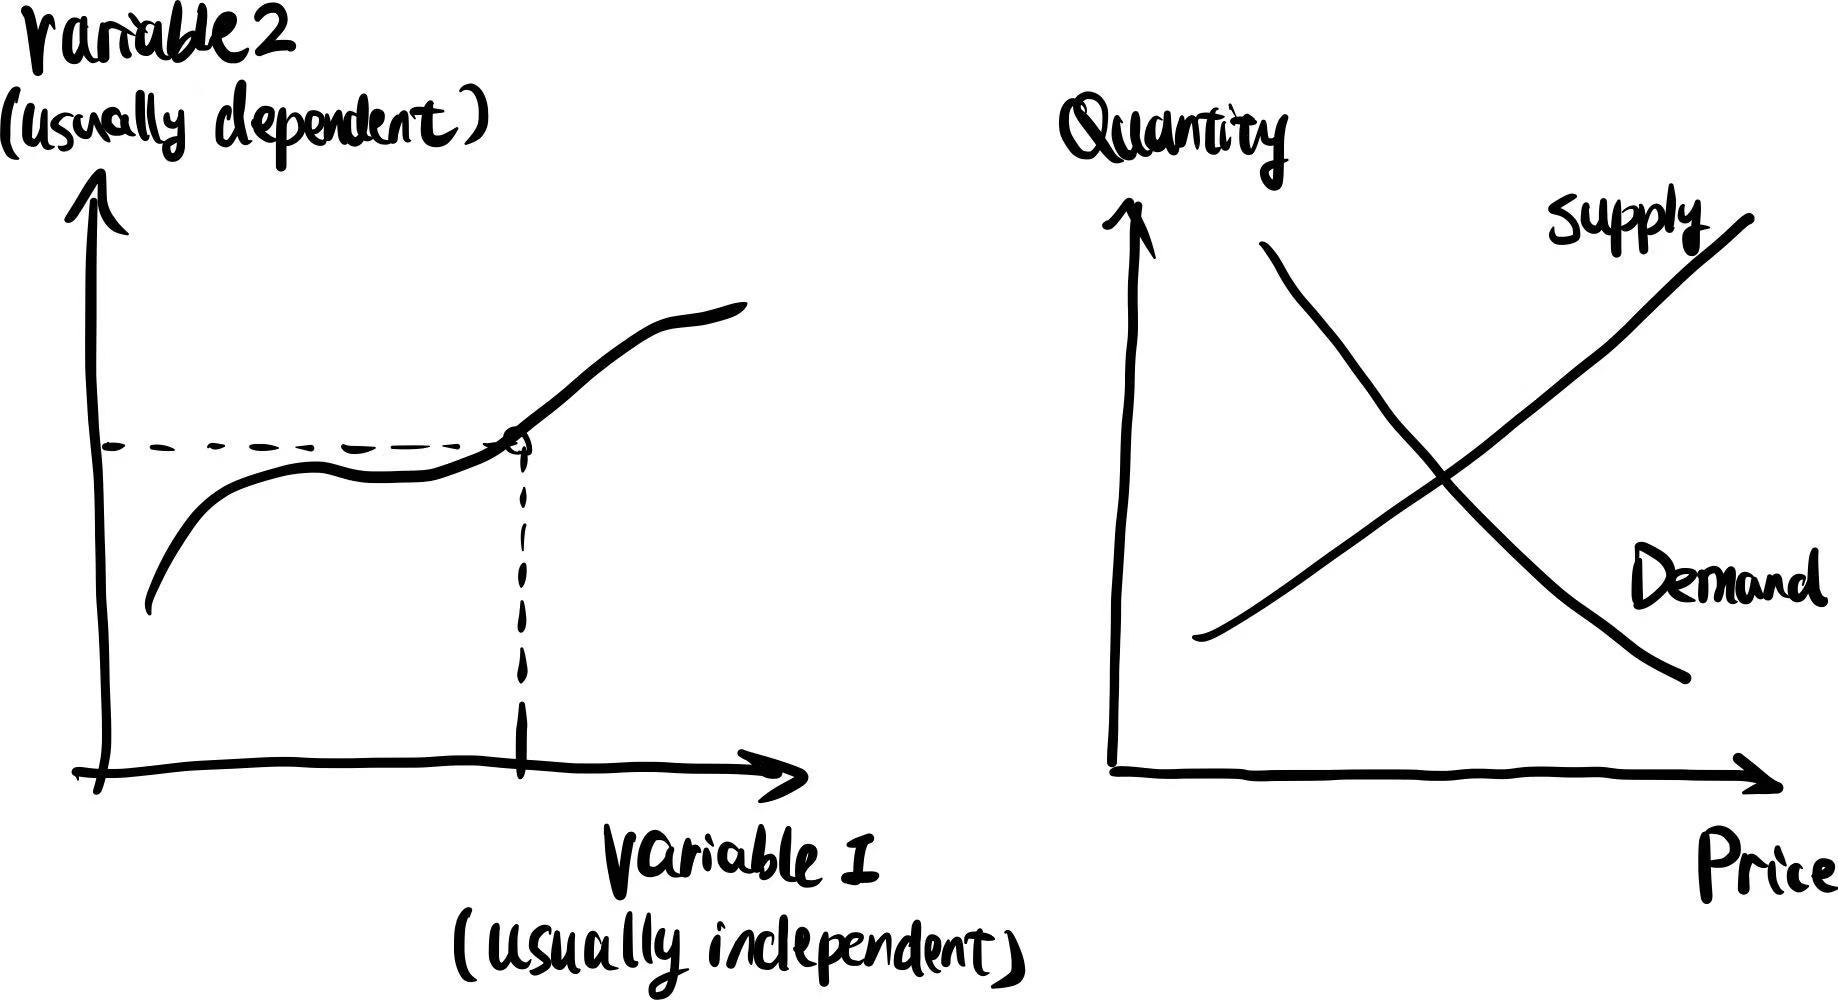
\includegraphics[width=0.9\textwidth]{img/image-20230228095149998.png}

\kaishu{\small 随着某商品的市场价格 (price) 增高, 生产者的生产意愿自然是增高的,
因为不考虑成本和其他因素变化的情况下 (Ceteris Paribus),
多生产的利润会更高, 因此供给曲线 (supply) 上扬, 反映出价格和供给量
(supply quantity) 的正相关; 另一方面,
消费者的消费意愿随着价格上涨自然是下降的, 于是需求曲线 (demand) 下压,
反映出价格和需求量 (demand quantity) 的负相关.

两条曲线分别对应着供给量和需求量关于价格的函数,
两函数的焦点反映了理想的自由市场下的最终成交价格和供需量
(因为在这个点达到了供需平衡 - equilibrium) ,
焦点向下作竖直线与横轴的焦点便显示了最终成交价格,
焦点向左作水平线与竖轴的交点便显示了平衡点的供需量.}
\end{tcolorbox}

在工程和计算机科学等思维里, 函数更像下左图所示, 给定一个输入 (input),
函数如同一台机器, 在加工后给出一个输出 (output); 这台机器非常可靠,
同样的输入能够稳定输出同样结果. 下右图给了一个例子

\begin{tcolorbox}[size=fbox, breakable, enhanced jigsaw]

\includegraphics[width=0.9\textwidth]{img/image-20230228095405809.png}

\kaishu{\small 假想有这样一个叫做``首都'' (Captital) 的函数,
放入一个国家名便会稳定输出这个国家的首都,
数学上我们可以这么标记下右图的例子 $\text{Capital(China)=Beijin}$.}
\end{tcolorbox}

函数的近现代定义和工科思维里的图景就很像, 考虑集合 $X$ 和 $Y$,
且它们不是空的, 如果存在某种特定的对应关系 $f$, 使得对于 $X$
中任意一个元素 $x$, 在 $Y$ 中都有唯一确定的元素 $y$ 和 $x$ 对应,
那么就称\textbf{映射} (mapping)\footnote{~Mapping 这个词用在这很贴切,
  map有地图的意思,
  ``映射''和地图上的每个点对应着实际区域上的一个个位置很相似.}
$f: A\rightarrow B$ 为从 $X$ 到 $Y$ 的一个函数, 记作
$y=f(x), x\in X$ 或者 $f(X)=\{y|f(x)=y, y\in Y\}$;
第一种记法强调元素的映射, 第二种记法强调整个集合的映射, $X$
在这里便是这个映射的定义域, $f(X)$ 是值域, $Y$
是这个映射的\textbf{陪域} (codomain, 也叫做上域, 到达域, 对应域),
大括号表示 $X$ 被映射到的集合, 其元素 $y$ 满足竖线后的条件, 即 $y$
是自 $x$ 通过 $f$ 这个映射得到, 并且 $y$ 属于 $Y$.
这样定义的直观感受类似下左图, 之前``首都''函数便类似下右图

\begin{tcolorbox}[size=fbox, breakable, enhanced jigsaw]
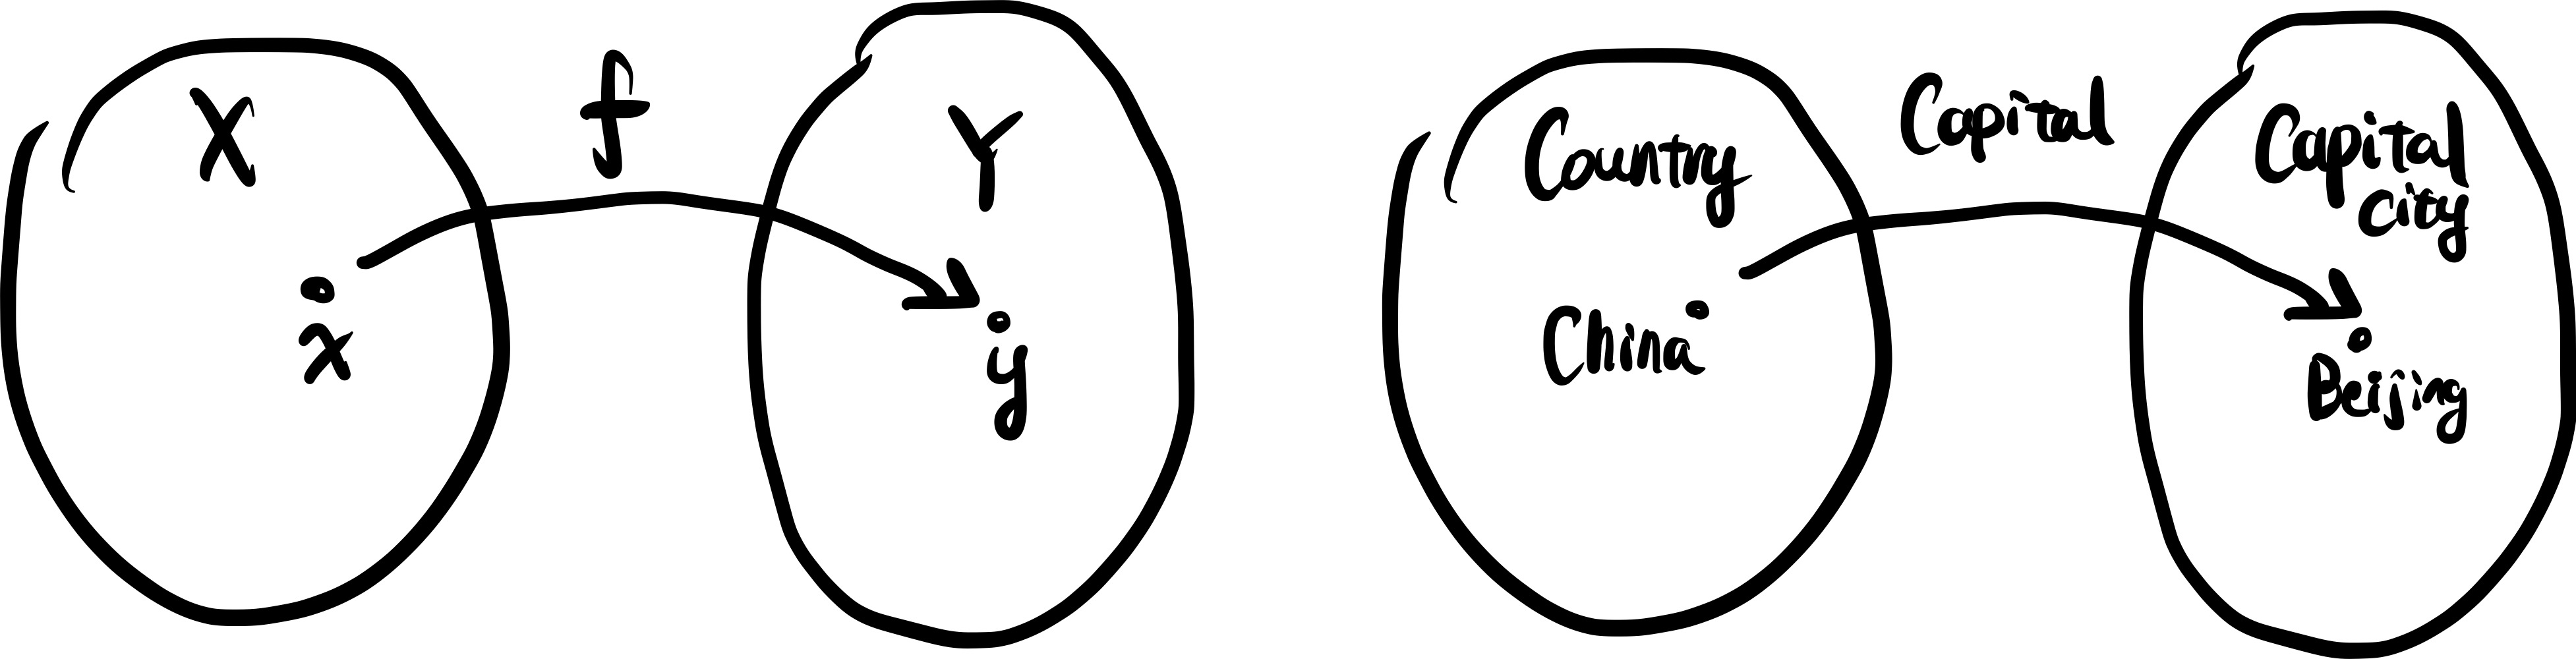
\includegraphics[width=0.9\textwidth]{img/image-20230228112941902.png}

\kaishu{\small Country这个集合里包含了很多国家, \{中国, 美国, 日本, \ldots\}; Capital
city这个集合里包含了很多城市, \{北京, 华盛顿, 东京, \ldots\};
Capital这个函数便描述了Country中的元素和Capital city中的元素的对应关系.}
\end{tcolorbox}

\end{tcolorbox}
\section{函数-下}\label{004}

\begin{flushright}{\kaishu 無名, 天地之始; 有名, 萬物之母. 常無, 欲以觀其妙; 常有, 欲以觀其徼. \\- 苏辙 『老子解』}\end{flushright}

\begin{tcolorbox}[size=fbox, breakable, enhanced jigsaw, title={单射, 满射, 双射 (injection, surjection,
bijection)}]

一个函数 $f:X\rightarrow Y$ 若满足, 如果 $a\neq b$ 则
$f(a)\neq f(b)$ 对于任何属于 $X$ 的 $a$ 和 $b$,
那么它便是\textbf{单射}的 (injection, one-to-one)\footnote{One-to-one
  是更``纯正''英语的说法, 比较通俗, injection 是来自法语的舶来词,
  更具高级感; 后面的 onto 和 surjection 同.}.

一个函数 $f:X\rightarrow Y$ , 若它的值域 (range) 和陪域 (codomain)
一致, 即对于任意 $y\in Y$, 都存在至少一个 $x\in X$ 满足
$f(x)=y$\footnote{介绍一下符号语言: $\exists$ - 存在; $\forall$ -
  对于所有. 于是这句话可以这么表述:
  $\forall y\in Y, \exists x\in X \text{ s.t. } f(x)=y$ (s.t.=such that
  可以译为``使得''). 但是通常情况下,
  还是尽量避免符号语言而使用自然语言来描述.}, 那么它便是\textbf{满射}的
(surjection, onto).

一个同时单射又满射的函数是\textbf{双射}的 (bijection, one-to-one
correspondance).

还是以Captial这个函数为例子, 下面给出了单射, 满射,
双射三种情况分别的图示:

\begin{tcolorbox}[size=fbox, breakable, enhanced jigsaw]
\begin{center}
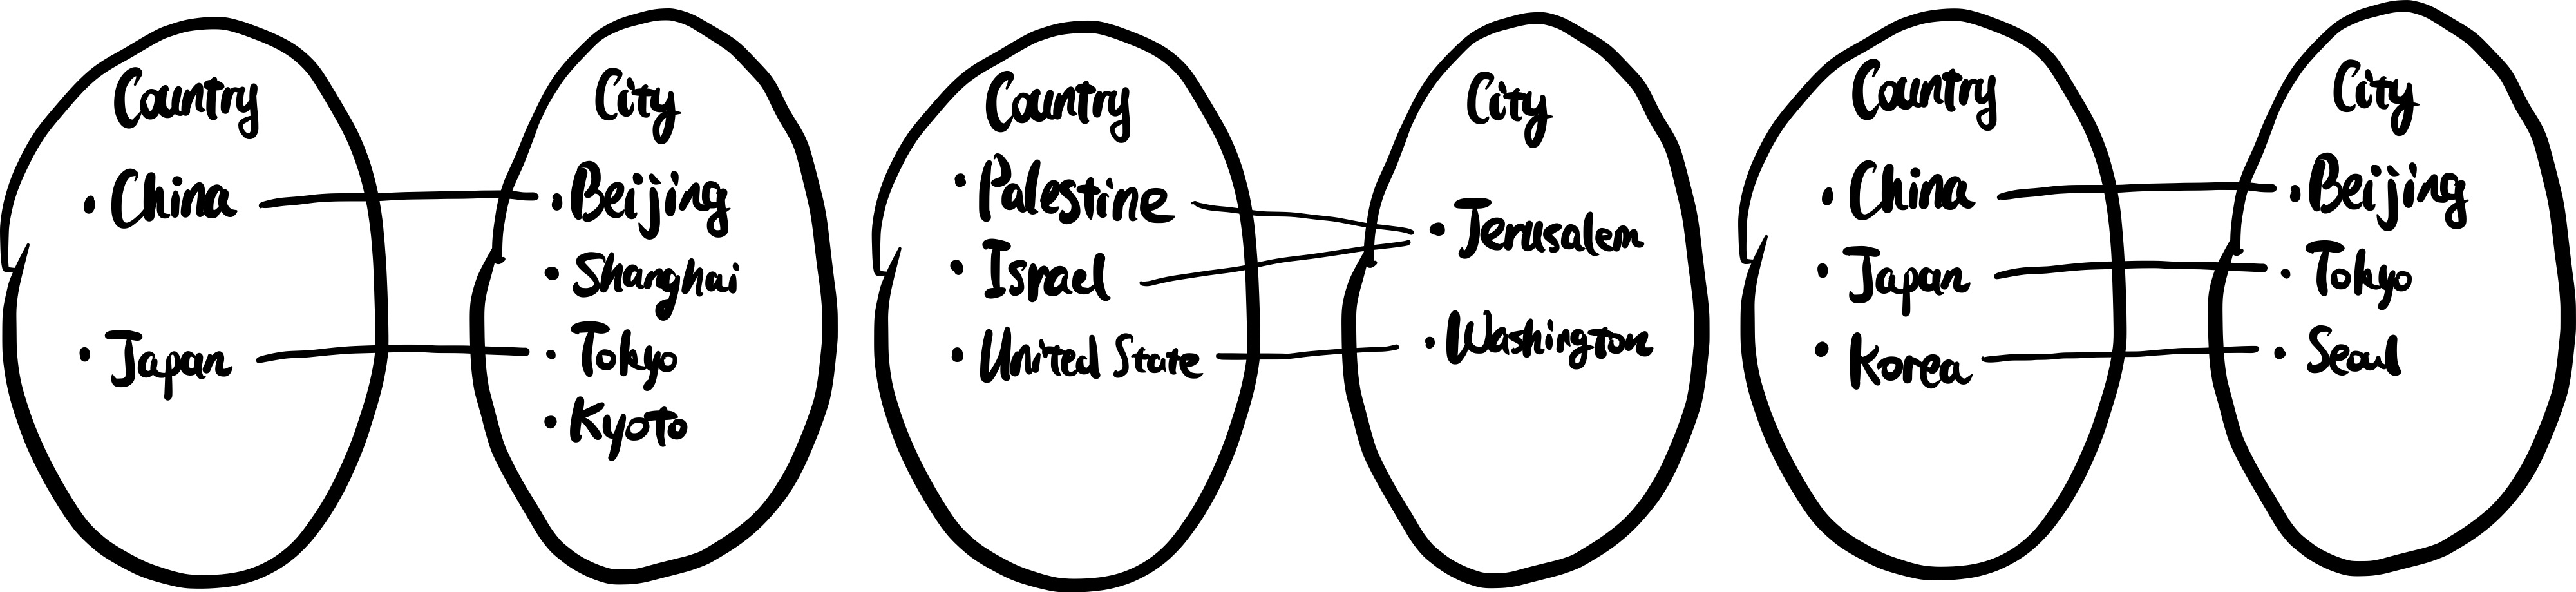
\includegraphics[width=0.9\textwidth]{img/image-20230302091706069.png}
\end{center}

\kaishu{\small 左: 单射但不满射; 中: 满射但不单射; 右: 双射.}
\end{tcolorbox}

\end{tcolorbox}

\begin{tcolorbox}[size=fbox, breakable, enhanced jigsaw, title={奇偶性 (parity 大嘘)}]

若一个函数满足 $f(-x)=-f(x)$, 即改变输入值 (自变量) 的正负号, 输出值
(因变量) 的正负号也改变, 这个函数便是\textbf{奇函数} (odd function).
图像上它是关于原点对称的.

若一个函数满足 $f(-x)=f(x)$, 即改变输入值 (自变量) 的正负号,
不影响输出值 (因变量) , 这个函数便是\textbf{偶函数} (even function).
图像上它是关于 $y$ 轴对称的.

当然, 奇函数和偶函数事实上是很特殊的两类函数,
更多的函数既不是奇函数又不是偶函数.

一些运算规律:

\begin{itemize}

\item
  奇函数 + 奇函数 = 奇函数\\{\kaishu 证明}: 假设存在两个奇函数 $f(x)$ 和
  $g(x)$, 令 $(f+g)(x) := f(x) + g(x)$, 即 $(f+g)(x)$
  这个函数是原本两函数之和. 根据奇函数的定义, $f(-x)=-f(x)$ 且
  $g(-x)=-g(x)$, 将两式相加得 $f(-x)+g(-x)=-f(x)-g(x)$, 即有
  $(f+x)(-x)=-(f+g)(x)$, 可见 $(f+g)(x)$ 是奇函数.
\item
  偶函数 + 偶函数 = 偶函数\\本条及接下来的证明与上一条类似, 可以当作练习.
\item
  奇函数 ×/÷ 奇函数 = 偶函数
\item
  偶函数 ×/÷ 偶函数 = 偶函数
\item
  奇函数 ×/÷ 偶函数 = 奇函数
\item
  偶函数 ×/÷ 奇函数 = 奇函数
\end{itemize}

\end{tcolorbox}

\begin{tcolorbox}[size=fbox, breakable, enhanced jigsaw, title={反函数 (inverse
function)}]

浅浅地非专业地叙述一下反函数. 设函数 $y=f(x)\ (x\in X)$ 的值域是
$Y$, 若存在一个函数 $g(y)$ 使得 $x= g(y)\ (y\in C)$, $g(x)$
便叫做 $f(x)$ 的\textbf{反函数} (inverse function), 可以记作
$x=f^{-1}(y)$, 它的定义域和值域分别是原函数的值域和定义域。

图像上, 反函数和原函数关于 $y=x$ 对称.

在求反函数时要特别注意反函数与原函数的定义域和值域. 例如 $y=f(x)=x^2$,
因为 $(\pm x)^2=y$, 反函数可能是 $x=f^{-1}(y)=\sqrt{y}$ 也可能是
$x=f^{-1}(y)=-\sqrt{y}$ , 但是不能是 $x=f^{-1}(y)=\pm\sqrt{y}$,
因为这样便不符合函数定义了, 一个输入值不可以有多个输出值,
或则说一个自变量不能对应多个因变量
(但是多个因变量对应一个自变量是允许的, 可以参考满射但不单射的图例).
这里反函数取正或负取决于原函数的定义域, 若 $y=f(x)=x^2, x\ge 0$, 则
$x=f^{-1}(y)=\sqrt{y}$; 若 $y=f(x)=x^2, x\le 0$, 则
$x=f^{-1}(y)=-\sqrt{y}$.

\end{tcolorbox}

\begin{tcolorbox}[size=fbox, breakable, enhanced jigsaw, title={隐函数 (implicit
function)}]

有的时候可能需要用函数来表达一个比较复杂的图像, 举一个简单一点的例子,
一个圆心位于原点的单位圆, 圆上任意一点到圆心距离都是 $1$, 于是有
$x^2+y^2=1$, 用前面学习的函数的形式表达这个关系, 有

$y=\begin{cases}\sqrt{1-x^2}\\-\sqrt{1-x^2}\end{cases}.$

这样似乎还没有起先的 $x^2+y^2=1$ 这个形式美观, 因此不妨还是用
$x^2+y^2-1=0$ 来表述单位圆上的 $x$ 与 $y$ 的关系. 类似这样,
利用一个【同时关于 $x$ 与 $y$ 的表达式 $F(x,y)=0$】来确定【 $y$
关于 $x$ 的函数】的表达式, 我们称之为\textbf{隐函数} (implicit
function); 为表区分, 前面介绍的类似 $y=f(x)$ 的函数,
称为\textbf{显函数} (explicit function).

\end{tcolorbox}

\begin{tcolorbox}[size=fbox, breakable, enhanced jigsaw, title={线性 (linearity)}]

这是一个很好的特性, 并不局限于函数, 仅对于函数来说的话,
若一个函数是线性的, 便有

$f(a+b)=f(a)+f(b),\ f(ax)=af(x).$

\end{tcolorbox}
\section{三角函数}\label{005}

\begin{flushright}{\kaishu 道可道, 非常道; 名可名, 非常名.}\end{flushright}

\begin{tcolorbox}[size=fbox, breakable, enhanced jigsaw, title={三角函数
(trigonometry)}]

三角函数最基本的使用应该是表示直角三角形的变长比. 如下图所示, 三角形
$ABC$ 为直角三角形, 将 $\angle BAC$ 记作 $\theta$, 对于两条直角边
$AB$ 和 $BC$, 边 $AB$ 在 $\theta$ 边上, 称它为\textbf{邻边}
(adjacent), 边 $BC$ 在 $\theta$ 对面, 称它为\textbf{对边}
(opposite), 剩余的边 $AC$ 被称为\textbf{斜边} (hypotenuse)。

\begin{tcolorbox}[size=fbox, breakable, enhanced jigsaw]
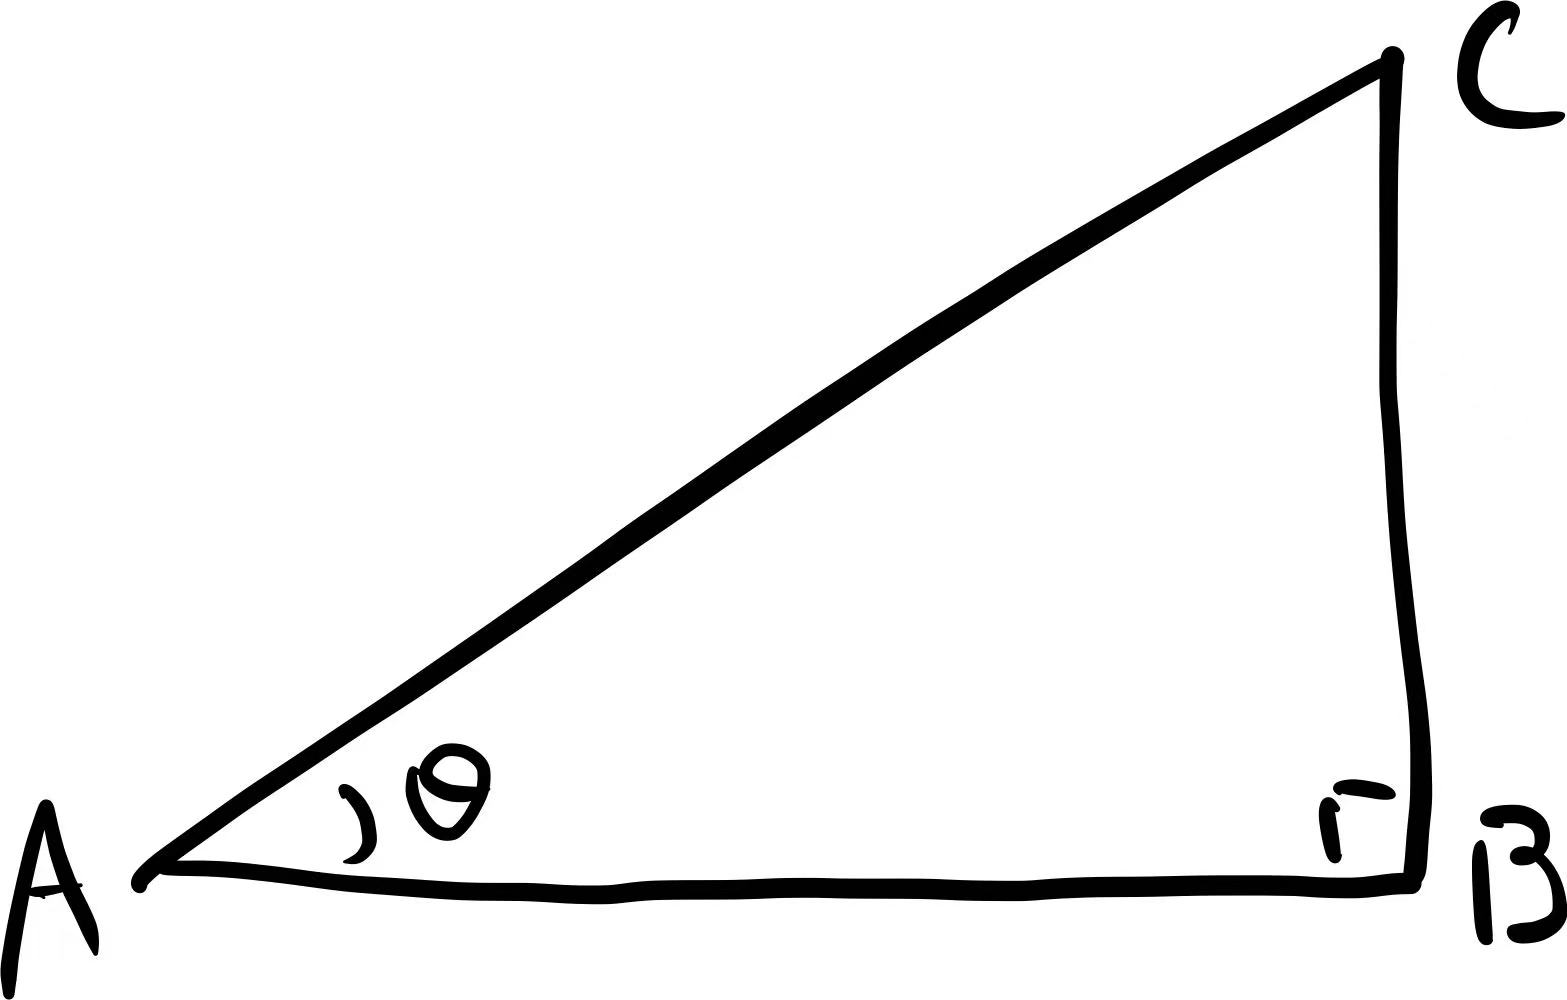
\includegraphics[width=0.5\textwidth]{img/image-20230308142717670.png}
\end{tcolorbox}

易见, 各变长比仅和 $\theta$ 相关\footnote{当然也可以说和除了直角外的另一个角
  $(90^\circ-\theta)$ 相关; 边长比可以通过一个除直角外的角确定是因为,
  除直角外另一角相等的直角三角形都相似, 它们的边长比是一致的。},
三角函数便是用来表示各个比例的, 常用的三角函数有

$\begin{aligned}\cos\theta&=\frac{\text{邻边}}{\text{斜边}}=\frac{AB}{AC},\\ \sin\theta&=\frac{\text{对边}}{\text{斜边}}=\frac{BC}{AC},\\ \tan\theta&=\frac{\text{对边}}{\text{邻边}}=\frac{BC}{AB}.\end{aligned}$

不难看出$\tan\theta=\frac{\sin\theta}{\cos\theta}$.

另外还有

$\begin{aligned}\sec\theta&\equiv\frac{1}{\sin\theta},\\ \csc\theta&\equiv\frac{1}{\cos\theta},\\ \cot\theta&\equiv\frac{1}{\tan\theta}.\end{aligned}$

$\csc$ 很多时候也记作 $\text{cosec}$.

一个非常实用的关系, 直角三角形中有\textbf{勾股定理} (Pythagorean
theorem): 斜边边长平方等于两直角边边长的平方之和, 即 $AC^2=AB^2+BC^2$;
两边同时除以 $AC^2$ 便有

\begin{itemize}

\item
  $\boxed{1=\cos^2\theta+\sin^2\theta}$.\footnote{三角函数的平方:
    cos(x)\textsuperscript{2} 通常理解为 cos((x)\textsuperscript{2});
    cos\textsuperscript{2}x 约定俗成表示 (cos(x))\textsuperscript{2}.}
\end{itemize}

\end{tcolorbox}

\begin{tcolorbox}[size=fbox, breakable, enhanced jigsaw, title={反三角函数}]

三角函数, 输入一个角度, 返回一个边长比; 反三角函数便是三角函数得逆运算,
或者说反函数 (参见【\ref{004}\nameref{004}】), 即输入一个边长比, 返回一个角度.

\end{tcolorbox}

\begin{tcolorbox}[size=fbox, breakable, enhanced jigsaw, title={正弦定律 (law of sine)}]

将三角形三个角分别记作 $\alpha$, $\beta$, 和 $\gamma$,
将它们的对边分别记作 $A$, $B$, 和 $C$. 先是结论:

\begin{itemize}

\item
  $\boxed{\frac{A}{\sin\alpha}=\frac{B}{\sin\beta}=\frac{C}{\sin\gamma}}$.
\end{itemize}

\begin{tcolorbox}[size=fbox, breakable, enhanced jigsaw]
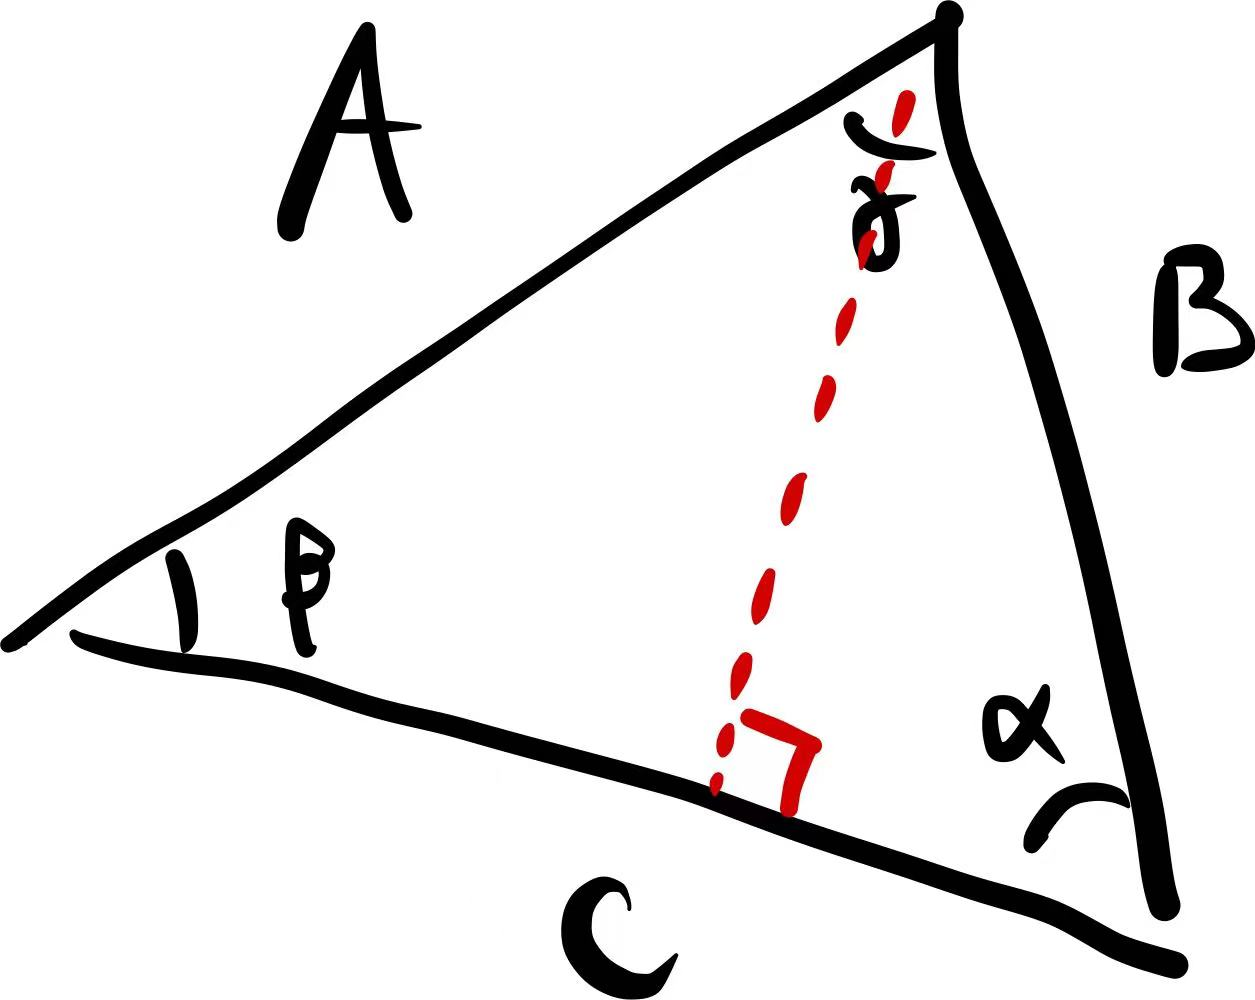
\includegraphics[width=0.5\textwidth]{img/image-20230308142913522.png}
\end{tcolorbox}

推导如下:

如上图所示, 以 $C$ 为底做高, 将原本的三角形分为左右两个直角三角形,
这条高利用左边的直角三角形可以表示为 $A\sin\beta$,
利用右边的直角三角形则是 $B\sin\alpha$, 于是有
$A\sin\beta=B\sin\alpha$, 整理可得
$\frac{A}{\sin\alpha}=\frac{B}{\sin\beta}$;
再做另一条高重复前面的操作, 便可得到完整的结论.

\end{tcolorbox}

\begin{tcolorbox}[size=fbox, breakable, enhanced jigsaw, title={余弦定律 (law of cosine)}]

还是先上结论:

\begin{itemize}

\item
  $\boxed{B^2=A^2+C^2-2AC\cos\beta}$,
\end{itemize}

即, 【一条边的边长平方】等于【另两条边的边长平方之】和加上【两倍的
(另两条边边长的乘积) 乘以 (另两条边的夹角的余弦)】.

\begin{tcolorbox}[size=fbox, breakable, enhanced jigsaw]
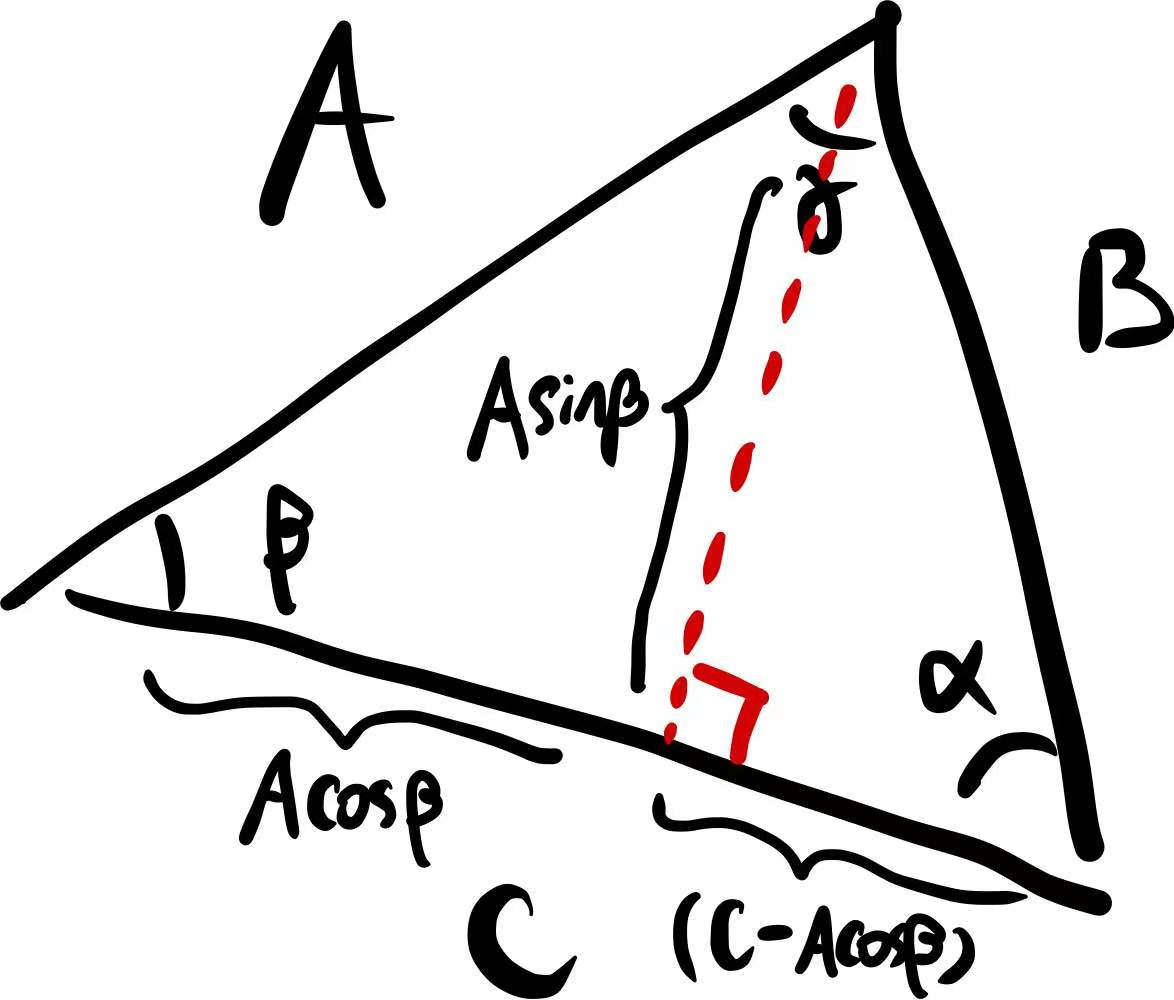
\includegraphics[width=0.5\textwidth]{img/image-20230308151417631.png}
\end{tcolorbox}

推导如下:

如下图所示, 依旧利用底边 $C$ 上的高将其分为左右两个直角三角形;
左边的直角三角形, 利用斜边 $A$ 和角 $\beta$, 两直角边分别可以表示为
$A\cos\beta$ 和 $A\sin\beta$, 于是右边的直角三角形边长便可表述为
$A\sin\beta$ 和 $(C-A\cos\beta)$; 对右边的直角三角形使用勾股定理

$\begin{aligned}B^2&=A^2\sin^2\beta+(C-A\cos\beta)^2\\ &=A^2\sin^2\beta+C^2+A^2\cos^2\beta-2AC\cos\beta\\ &=A^2+C^2-2AC\cos\beta.\end{aligned}$

其中等式的后两行用到了之前得出的 $1=\cos^2\theta+\sin^2\theta$.

\end{tcolorbox}

\begin{tcolorbox}[size=fbox, breakable, enhanced jigsaw, title={任意角度的三角函数}]

不难发现, 前面讨论的情况似乎都是锐角的情况 (主要是因为插图\ldots),
钝角的三角函数似乎没那么直观了, 因为做不成一个含有钝角的直角三角形,
没法简单地用边长比来表示 $\sin$ 和 $\cos$ 等. 于是,
我们需要想办法将前面的情形推广.

如下左图所示, 建立直角坐标系, 做一圆心位于原点的单位圆, 即半径为 $1$
的圆, 考虑在第一象限的圆上的一点, 将其与原点做连线, 将从
$x$-轴正方向与这条连线\textbf{顺时针}方向形成的夹角记作 $\theta$,
不难看出这个点的坐标 $(x,y)$ 满足

$\begin{cases}x=\cos\theta,\\y=\sin\theta.\end{cases}$

\begin{tcolorbox}[size=fbox, breakable, enhanced jigsaw]
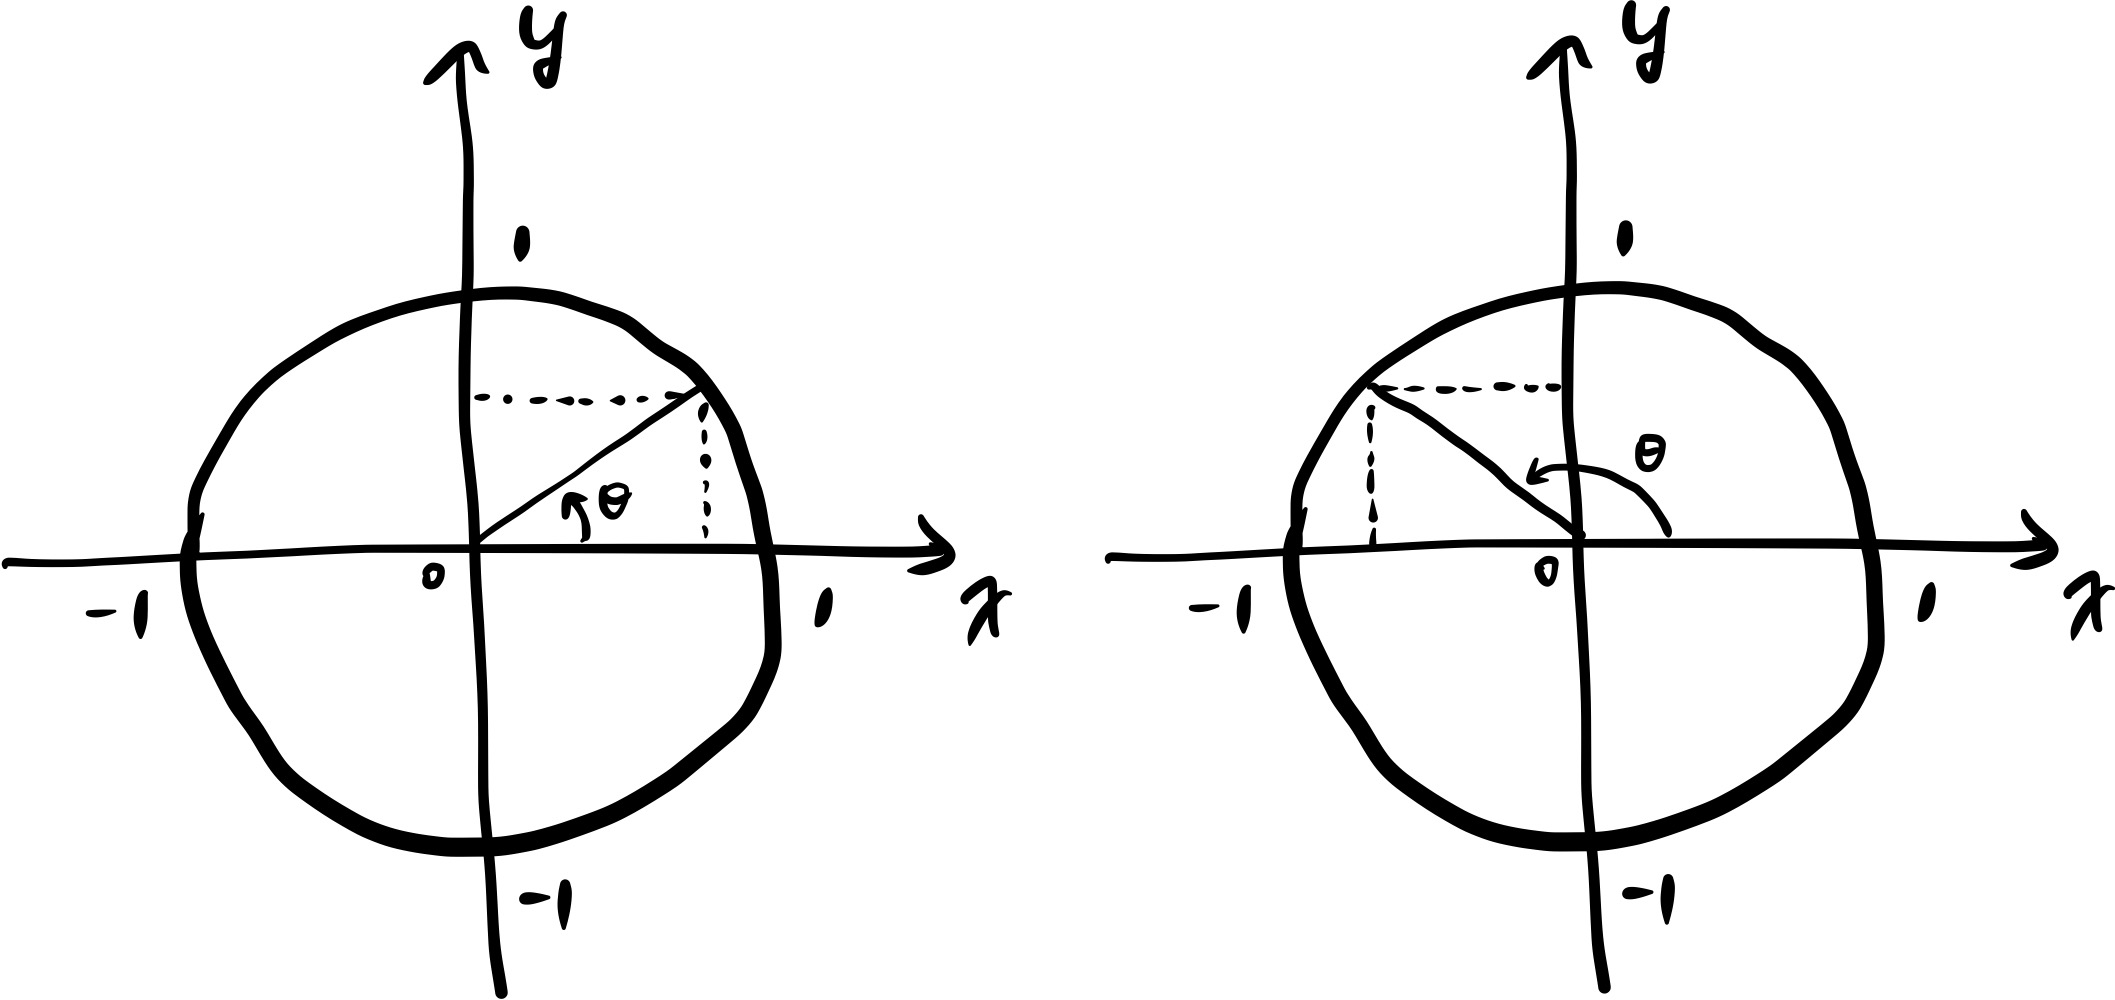
\includegraphics[width=0.75\textwidth]{img/image-20230316171124433.png}
\end{tcolorbox}

于是不妨将其他象限的情况也按此定义,
于是如上右图所示的钝角甚至更大角度的三角函数便可以被定义了.

\end{tcolorbox}

\begin{tcolorbox}[size=fbox, breakable, enhanced jigsaw, title={弧度制 (radian)}]

为什么一个周角是 $360^\circ$ 呢, 听说过一个不可考的说法: $360$
是一个有很多因数的数字 (1, 2, 3, 4, 5, 6, 8, 9, 10, 12\ldots),
等分起来的时候数字会比较友好, 所以 $360^\circ$ 其实是非常随意地规定的.
那么有没有更好的用来描述角度方法呢? 答案是弧度.

一个半径为 $r$ 的圆的周长是 $2\pi r$, 一个圆心角为 $n^\circ$
的扇形的弧长是 $2\pi r\frac{n}{360}$. 可见圆心角越大弧越长,
且圆心角和弧长成正比. 既然如此,
不如重新将角度定义为圆心角与弧长的比值以方便计算, 于是便有了,
在新的这套单位系统中, 若圆心角大小为 $\theta$, 其对应弧长应为
$r\theta$; 当圆心角是一个周角时, 对应弧长便成了圆的周长 $r(2\pi)$.
所以角度和这个新的单位的换算有 $360^\circ\equiv 2\pi\ \text{rad}$,
因为这个单位把圆心角和对应的弧长联系起来了, 因此称之为\textbf{弧度}
(radian).

扇形面积在这套单位制, 即弧度制下, 便也成了 $\frac{1}{2}r^2\theta$.

\end{tcolorbox}

\begin{tcolorbox}[size=fbox, breakable, enhanced jigsaw, title={三角函数的图像}]

现在这个时代, 大家都或多或少能接触到科学计算器,
再不济在bing.com上搜索``solver''用微软的 Microsoft Solver
也可以计算某个特定角度的三角函数值, 自然也可以绘制函数图像.
下图分别展示了 $\sin(x)$ 和 $\cos(x)$ 的图像,

\begin{tcolorbox}[size=fbox, breakable, enhanced jigsaw]
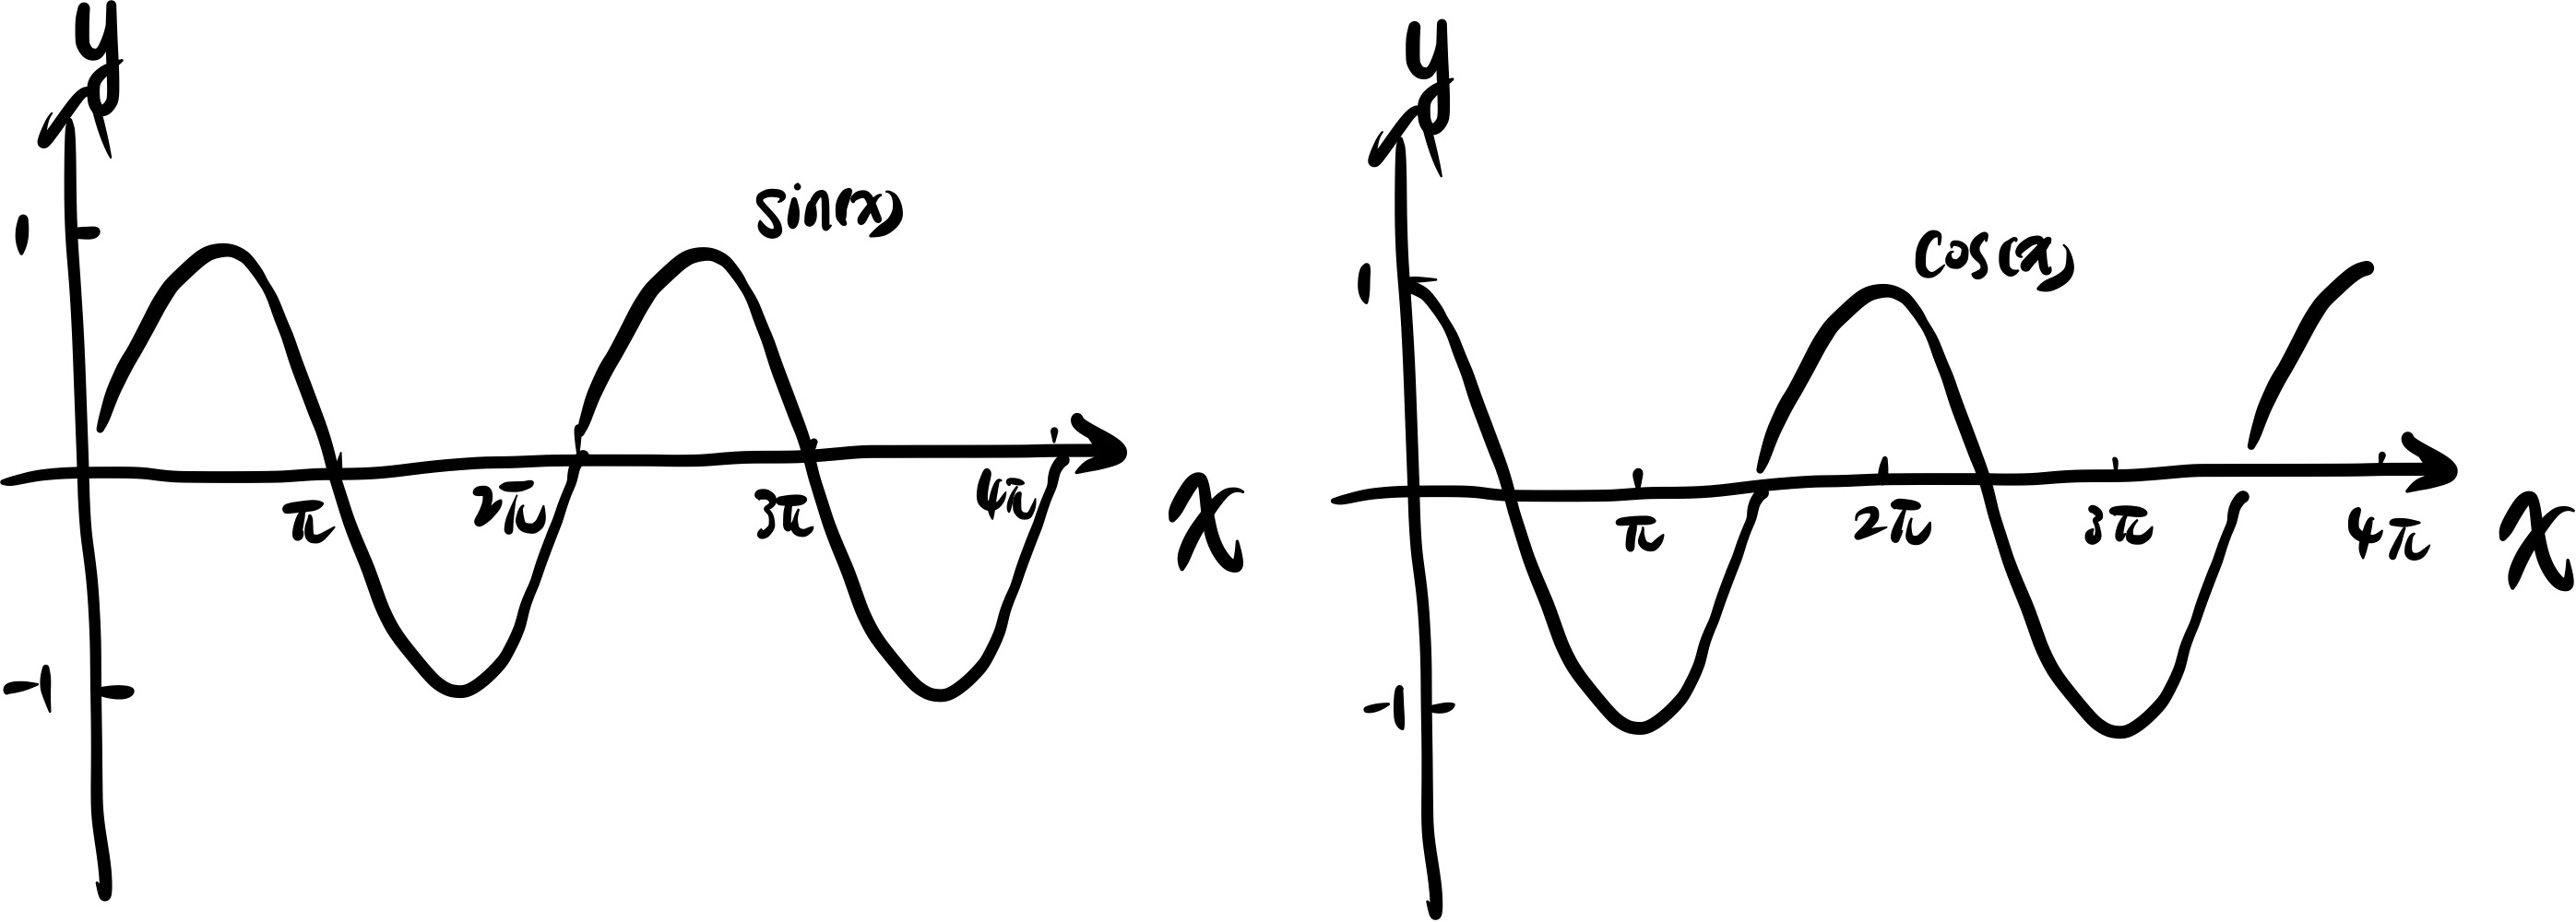
\includegraphics[width=0.75\textwidth]{img/image-20230316171137500.png}
\end{tcolorbox}

一些值得关注的点是它们都是\textbf{周期函数} (periodic function),
随着自变量-角度的变化, 因变量-函数值的变化是周期性的, 它们的周期都是
$2\pi$, 这一点从上文的单位圆里便可看出些许原因,
当角度变化超过一个周角时, 和角度刚从 $0$ 开始的情况是一样的.

\end{tcolorbox}
\section{虚数和复数}\label{006}

\begin{flushright}{\kaishu 些许绕行 (detour).}\end{flushright}

\begin{tcolorbox}[size=fbox, breakable, enhanced jigsaw, title={虚数和复数 (imaginary number and complex number)}]

考虑一个一元二次方程 $ax^2+bx+c=0$, 它的解有

$\begin{aligned}
0&=a\left(x^2+\frac{b}{a}x+\frac{c}{a}\right)\\
0&=x^2+\frac{b}{a}x+\frac{c}{a}\\
0&=x^2+\frac{b}{a}x+\left(\frac{b}{2a}\right)^2-\left(\frac{b}{2a}\right)^2+\frac{c}{a}\\
0&=\left(x-\frac{b}{2a}\right)^2-\left(\frac{b}{2a}\right)^2+\frac{c}{a}\\
\left(x-\frac{b}{2a}\right)^2&=\left(\frac{b}{2a}\right)^2-\frac{c}{a}\\
&...\\
x&=\boxed{\frac{-b\pm\sqrt{b^2-4ac}}{2a}}.
\end{aligned}$

上式最后的结论便是求根公式, 不难看出整个推导过程实际上就是配方,
其中根号前面的``加减''是因为对等式两边同时开方时,
正负两种情况都是正确的.

我们在此之前接触到的数字都还限于实数范围内, 因此会要求
$\left(b^2-4ac\right)$ 是正的, 以保证开方之后的结果是``有意义的'',
然而

\begin{newquote}
    ``从来如此, 便对么?''
\end{newquote}

之前也出现了, 不能被表示成分数形式的数字,
我们的研究范围从有理数扩充到了实数; 现在, 若 $\left(b^2-4ac\right)$
是负的, 按照当前的理解, 它不能被开方, 那是不是又到了这样一个神圣的时刻,
我们需要拓展我们研究的数字的范围?

既然如此, 不如规定 $\sqrt{-1}\equiv i$, 作为新的一类数字的单位,
因为之前的数字叫``实数'', 那么这一类新的数字就不妨叫做``\textbf{虚数}''
(imaginary number) 吧. 一个既包含实数部分, 又包含虚数的部分的数字,
我们就叫它``\textbf{复数}'' (complex number), 记作 $\mathbb{C}$.
\end{tcolorbox}

\begin{tcolorbox}[size=fbox, breakable, enhanced jigsaw, title={运算规律}]

考虑若干个复数, $z_1=a+bi$, $z_2=c+di$, $z_3=e+fi$\ldots{}

\begin{itemize}

\item
  \textbf{加法}: $z_1+z_2=(a+c)+(b+d)i$.
  实数部分和虚数部分可以分开计算,
  应该不难看出复数和加法是构成\textbf{阿贝尔群}的
  (即它具有封闭性和结合律, 有单位元和逆元, 并且有交换律, 详细参见\ref{001}\nameref{001}).
\item
  \textbf{乘法}:
  $z_1\times z_2=(a+bi)\times(c+di)\\=ac+adi+bci+bdi^2=(ac-bd)+(ad+bc)i.$
  不难看出, 复数和乘法也构成阿贝尔群.
\item
  乘法对于加法满足\textbf{分配律}, 即,
  $(z_1+z_2)\times z_3=z_1\times z_3+z_2\times z_3$,
  证明留作练习\footnote{事实上, 很多情况下, 之前提到的很多知识点,
    例如单位元, 零元, 逆元都分左右, 分配律也有左分配律和右分配律,
    但是目前讨论的情况都是满足交换律的, 所以可以不区分左右.}.
\end{itemize}

以上三条已经足够使得复数与加法和乘法构成一个\textbf{环} (ring), 事实上,
环只需要乘法是半群 (semi-group, 即满足结合律和有单位元的二元运算与集合) 即可.

\begin{itemize}

\item
  \textbf{减法}: 因为加法存在逆元, 所以减去一个数,
  可以视作加上这个数的加法逆元, 即:
  $z_1-z_2=(a+bi)-(c+di)\\\Rightarrow z_1+(-z_1)=(a+bi)+(-(c+di))=(a-c)+(b-d)i$
\item
  \textbf{除法}: 不难发现每个非零的元素都有乘法逆元,
  因此除以一个数可以视作乘上这个数的乘法逆元, 即: 因为
  $z_2\times\frac{1}{z_2}=\frac{c+di}{c+di}=1$, 于是
  $z_1\div z_2=z_1\times\frac{1}{z_2}=\frac{a+bi}{c+di}$.
\end{itemize}

\begin{newquote}
一点小插曲, $\frac{a+bi}{c+di}$ 应该怎么化简呢,
怎么写成简单的实数部分加上虚数部分的形式呢?
回顾一下无理数的``分母有理化'', 例如有
$\frac{a+\sqrt{b}}{c+\sqrt{d}}$, 我们会将分子分母同时乘以
$(c-\sqrt{d})$ 将分母变为有理数, 便有
$\frac{(a+\sqrt{b})(c-\sqrt{d})}{c^2-d}$. 类似的, 当我们尝试化简
$\frac{a+bi}{c+di}$时, 我们也不妨对分子分母同时乘以 $(c-di)$, 于是有
$\frac{(a+bi)(c-di)}{c^2+d^2}$, 分母便变为了实数,
再稍加化简便可转化为一个实数加上一个虚数的形式. 我们称 $(c-di)$ 是
$(c+di)$ 的\textbf{复共轭} (complex conjugate)\footnote{两头牛背上的架子称为轭,
  轭使两头牛同步行走. 共轭就描述了两个对象这样一种相生相随的关系.}.
\end{newquote}

像上述这样可以进行加减乘和除零外除法,
并满具足一些特定的阿贝尔群的特点和分配律的代数结构,
换言之一个满足交换律的环 (交换环 commutative ring)
附加上除零外元素的除法运算, 构成一个\textbf{域} (field), 可以记作
$\mathbb{F}$, 常见的例子有有理数域, 实数域, 复数域.

\begin{tcolorbox}[size=fbox, breakable, enhanced jigsaw]
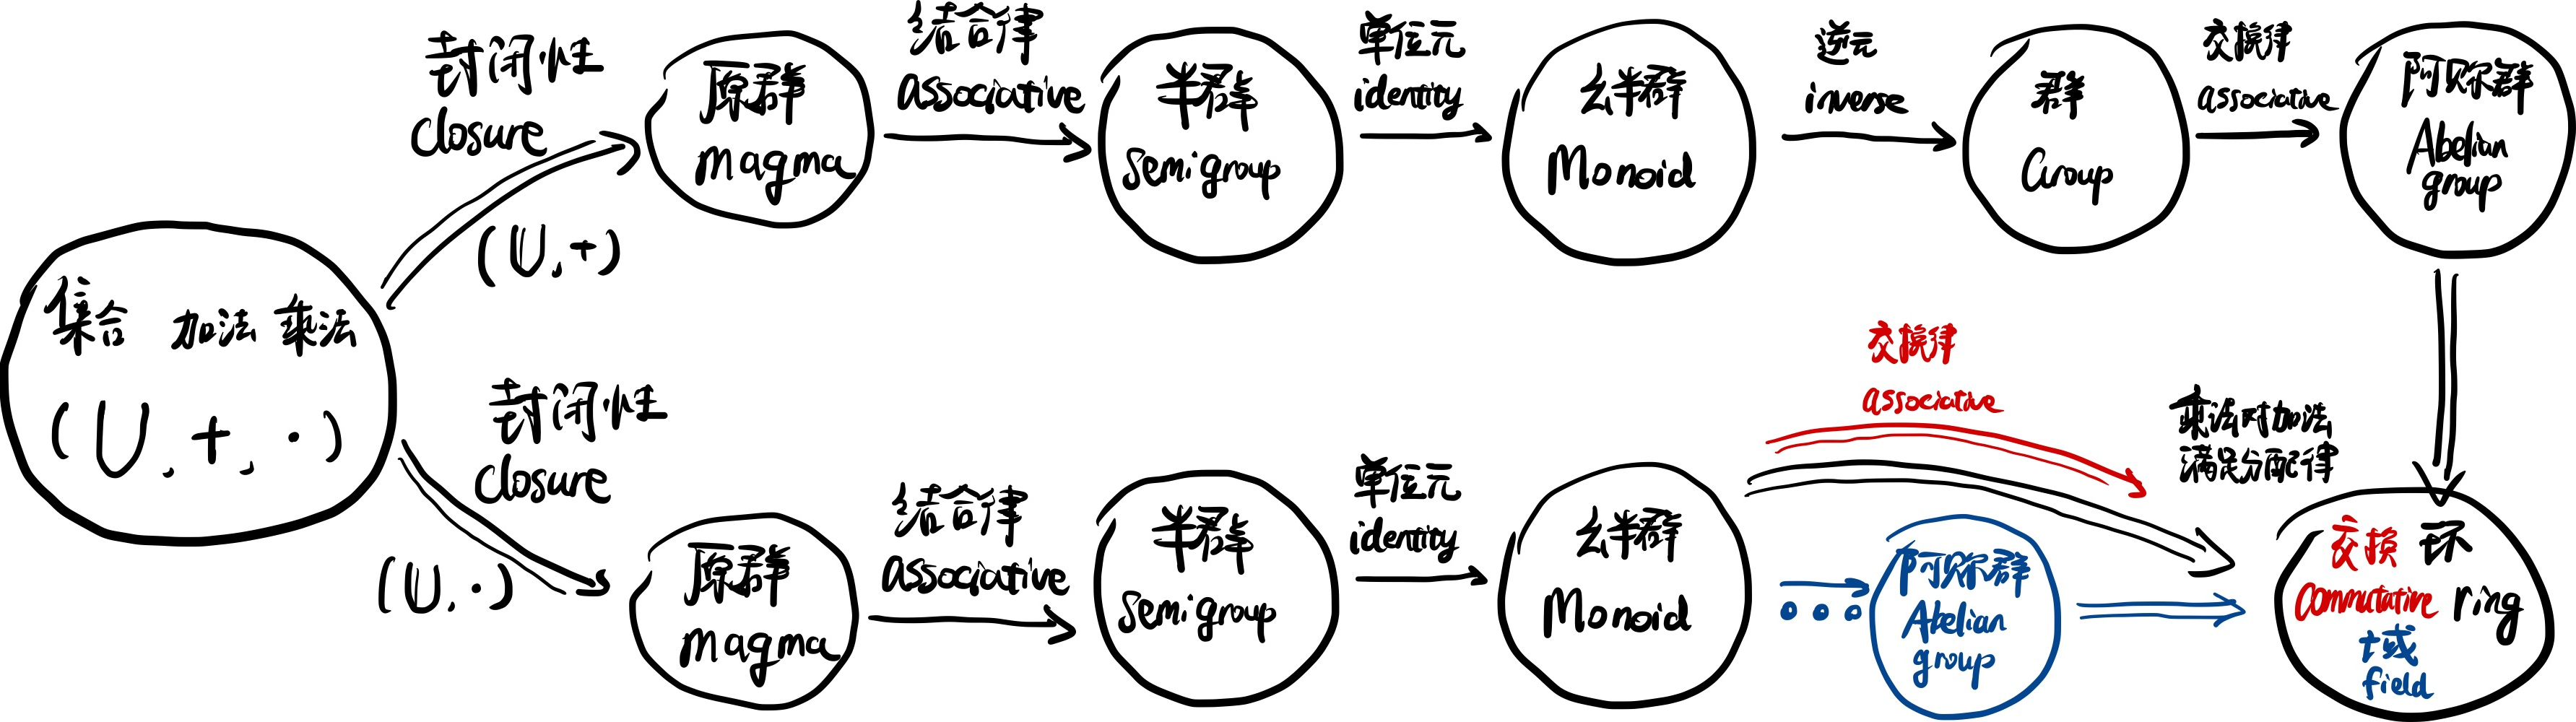
\includegraphics[width=0.9\textwidth]{img/image-20230328100716650.png}

\kaishu{\small 环, 交换环, 域的关系, 图改自知乎@SparkAndShine}
\end{tcolorbox}

\end{tcolorbox}
\begin{quote}
绕行之绕行 (detour of the detour).
\end{quote}

\hypertarget{ux4e8cux9879ux5f0fux5c55ux5f00-binomial-expansion}{%
\subsubsection{二项式展开 (binomial
expansion)}\label{ux4e8cux9879ux5f0fux5c55ux5f00-binomial-expansion}}

\textbf{二项式展开}指的是将类似 \((x+y)^n\) 的表达式展开的过程. 结论上有

\(\boxed{(x+y)^n=\sum_{r=0}^n\binom{n}{r}x^{n-r}y^r}.\)

这里 \(\binom{n}{r}=\frac{n!}{r!(n-r)!}\) 也记作 \(_nC_r\),
这个''C''是\textbf{组合} (combination) 的意思, 其中又有
\(n!=n\times(n-1)\times...\times3\times2\times1\).

\begin{quote}
上面第一次出现了求和符号 \(\sum\), 在此用一些例子说明,

\(\sum_{i=1}^{10}i=1+2+3+...+9+10;\)

\(\sum_{x=1}^{10}x^2=\left.x^2\right|_{x=1}+\left.x^2\right|_{x=2}+...+\left.x^2\right|_{x=10}=1^2+2^2+...+10^2.\)

即, 求和符号后的表达式, 依次代入求和符号下方的值,
符号下方的值加一\ldots, 直至代入求和符号上方的值, 最后将这些项求和.
\end{quote}

二项式展开的证明思路如下:

\textbf{从组合的思路出发}

\begin{itemize}
\item
  将 \((x+y)^n=\underbrace{(x+y)(x+y)...(x+y)}_{n}\) 展开,
  并将同类项合并, 易见可能出现的项的形式仅为 \(x^n=x^ny^0\),
  \(x^{n-1}y=x^{n-1}y^1\), \(x^{n-2}y^2\), \ldots{} \(x^2y^{n-2}\),
  \(xy^{n-1}=x^1y^{n-1}\), \(y^n=x^0y^n\).
\item
  合并后这些项的系数是合并前它们分别出现的次数,

  \begin{itemize}
  \tightlist
  \item
    \(x^n\) 相当于展开时每一个 \((x+y)\) 都选取 \(x\) 的情况,
    只有一种这样的情况, 即合并前 \(x^n\) 只可能出现 \(1\) 次,
    那么合并后它的系数便是 \(1\).
  \item
    \((x^{n-1}y^1)\) 相当于展开时每一个 \((x+y)\) 选取了 \((n-1)\) 个
    \(x\) 和 \(1\) 个 \(y\), 利用组合学的知识有
    \(n=\frac{n!}{1!(n-1)!}\) 种这样的情况, 即合并前 \((x^{n-1}y^1)\)
    出现 \(n\) 次, 那么合并后它的系数便是 \(n\).
  \end{itemize}

  \begin{quote}
  这个 \(n\) 可以这么看待, 选取的这个 \(y\) 可以出自这 \(n\) 项
  \((x+y)\) 中的任意一个, 于是便有 \(n\) 种可能.
  \end{quote}

  \begin{itemize}
  \tightlist
  \item
    \((x^{n-2}y^2)\) 相当于展开时每一个 \((x+y)\) 选取了 \((n-2)\) 个
    \(x\) 和 \(2\) 个 \(y\), 利用组合学的知识有
    \(\frac{n(n-1)}{2!}=\frac{n!}{1!(n-1)!}\) 种这样的情况, 即合并前
    \((x^{n-1}y^1)\) 出现 \(n\) 次, 那么合并后它的系数便是 \(n\).
  \end{itemize}

  \begin{quote}
  这个 \(\frac{n(n-1)}{2!}\) 可以这么看待, 选取的这两个 \(y\) 可以出自这
  \(n\) 项 \((x+y)\) 中的任意两个, 第一个 \(y\) 有 \(n\) 种选法,
  第二个因为第一个''占用''了一个 \((x+y)\), 因此它只有 \((n-1)\) 种选法,
  综上便有了 \(n(n-1)\); 然后两个 \(y\) 的顺序是无所谓的, 两个 \(y\)
  本身先后的排序会额外引入一个倍数 \(2\), 于是除掉.
  \end{quote}

  \begin{itemize}
  \tightlist
  \item
    \ldots{}
  \item
    \((x^{n-r}y^r)\) 相当于展开时每一个 \((x+y)\) 选取了 \((n-r)\) 个
    \(x\) 和 \(r\) 个 \(y\), 利用组合学的知识有
    \(\frac{n(n-1)...(n-r)}{(n-r)!}=\frac{n!/r!}{(n-r)!}=\frac{n!}{1!(n-1)!}=\binom{n}{r}\)
    种这样的情况, 即合并前 \((x^{n-1}y^1)\) 出现 \(\binom{n}{r}\) 次,
    那么合并后它的系数便是 \(\binom{n}{r}\).
  \end{itemize}

  \begin{quote}
  这个 \(\frac{n(n-1)...(n-r)}{(n-r)!}\) 可以这么看待, 选取的这 \(r\) 个
  \(y\) 可以出自这 \(n\) 项 \((x+y)\) 中的任意 \(r\) 个, 第一个 \(y\) 有
  \(n\) 种选法, 第二个因为第一个''占用''了一个 \((x+y)\), 因此它只有
  \((n-1)\) 种选法, 第三个于是只有 \((n-2)\) 种\ldots{} 综上便有了
  \(n(n-1)...(n-r)\); 然后 \(r\) 个 \(y\) 的顺序是无所谓的, \(r\) 个
  \(y\) 本身先后的排序, 第一个 \(y\) 顺序可能是 \(1\) 至 \(r\), 有 \(r\)
  种选择, 第二个只有 \((r-1)\)\ldots{} 于是会额外引入一个倍数
  \(r(r-1)...1=r!\), 于是除掉.
  \end{quote}
\item
  可见某一项 \((x^{n-r}y^r)\), 系数应为 \(\binom{n}{r}\), \(r=0\) 至
  \(r=n\) 的项都是允许的, 于是利用求和符号表示, 便有了最开始的结论.
\end{itemize}

这样的思路也可以推出杨辉三角 (Pascal's Triangle):

\begin{Shaded}
\begin{Highlighting}[]
    \FloatTok{1}
   \FloatTok{1}  \FloatTok{1}
  \FloatTok{1}  \FloatTok{2}  \FloatTok{1}
 \FloatTok{1}  \FloatTok{3}  \FloatTok{3}  \FloatTok{1}
\FloatTok{1}  \FloatTok{4}  \FloatTok{6}  \FloatTok{4}  \FloatTok{1}
\end{Highlighting}
\end{Shaded}

三角的左右两边由 \(1\) 填满, 中间的某个数字是左上和右上两个数字之和.
不难发现, 从第二行开始, 每一行的数字是都是二项式展开的系数.

上述的推导, 和类似【抛 \(n\) 次公平的硬币, 得到 \(r\) 次正面和 \((n-r)\)
次反面】的场景有着非常深的联系, 这里暂时不做展开.

\textbf{数学归纳法}

这个方法一般只能用于证明, 不能用于推导.

\begin{quote}
\textbf{数学归纳法} (proof by induction) 思路如下

\begin{enumerate}
\def\labelenumi{\arabic{enumi}.}
\tightlist
\item
  \textbf{归纳奠基} (base case), 证明第一个情况是对的;
\item
  归纳递推, 假设第 \(n\) 个情况正确, 以此推出第 \((n+1)\) 个情况正确,
  便有所有情况都成立.
\end{enumerate}

已知若情况n成立便有情况(n+1)也成立; 因为有情况1成立, 于是代入n=1,
便有情况2也成立; 现在知道情况2也成立了, 继续代入n=2,
便有情况3也成立\ldots{}
\end{quote}

思路已经给到, 具体证明留作练习. 一点提示是
\(\binom{r}{n+1}=\binom{r}{n}+\binom{r-1}{n}\).

\textbf{应用}

除了常规的 \(n\) 是整数的一些应用, 在保证展开的形式是\textbf{收敛}
(coverge) 的情况下 (即求和的形式不会趋向于正/负无穷),
二项式展开的负整数, 甚至分数形式也是成立的.

例如狭义相对论 (special relativity) 中, 随着物体运动速度变化,
物体的相对论性质量 (relativitic mass)\footnote{静止质量是物体静止时的质量,
  或者说某个观察者发现某物体处于静止状态下时这个物体的质量;
  相对论性质量则是物体相对观察者具有一定速度时, 观察者观察到的质量.}会变大,
它和静止质量 \(m_0\) 符合关系式

\(m=\frac{m_0}{\sqrt{1-v^2/c^2}}.\)

上式中 \(v\) 时速度, \(c\) 是光速. 根据幂运算的规律 (复习【002】),
上式可以改写成

\(m=m_0(1-v^2/c^2)^{-1/2}.\)

在估算例如速度在 \(0.01c\) 或更小时, 相对论性质量与静止质量之差,
直接计算 \((m-m_0)\) 通常看不出 \(m\) 与 \(m_0\) 的区别\footnote{计算机保存的并不是准确值,
  而是浮点数 (暂不展开), 可以暂且不太正确但道理就这么个道理地理解为:
  它保存的答案是一个写成科学计数法的数值, 并且位数有限,
  超过一定位数的部分就被切掉了;
  于是两个很接近的数字在计算机看来有可能是相等的, 进而计算不出差值.};
事实上, 我们可以利用二项式展开, 因为

\((1+x)^n=1+nx+\frac{n(n-1)}{2!}x^2+...,\)

代入 \(x=(v^2/c^2)\) 与 \(n=\frac{1}{2}\) 便有

\(m=m_0\left(1+(-1/2)\left(-\frac{v^2}{c^2}\right)+\frac{(-1/2)(-1/2-1)}{2!}\left(-\frac{v^2}{c^2}\right)^2\right)=m\left(1+\frac{v^2}{2c^2}+\frac{3}{8}\frac{v^4}{c^4}+...\right).\)

这个形式下, 相对论性质量与静止质量之差就很明显

\(m\left(\frac{v^2}{2c^2}+\frac{3}{8}\frac{v^4}{c^4}+...\right),\)

利用前几项便可以得到很好的近似.

绕行似乎要结束了, 之前的铺垫使得接下来的道路逐渐明朗\ldots{}

\hypertarget{ux81eaux7136ux5e38ux6570-natural-constant}{%
\subsubsection{自然常数 (natural
constant)}\label{ux81eaux7136ux5e38ux6570-natural-constant}}

通常自然常数会以下面两个例子引出:

\textbf{复利}

考虑一个奇怪的银行, 年利率是 \[100\%\], 也就是说, 存入 \[1\] 个货币,
到了年底便有

\[1\times(1+100\%)=2.\]

更奇怪的一点, 这家银行的单位时间利率不会因为存款周期改变, 也就是说, 存
\[0.5\] 年的利率是 \[0.5\times100\%=50\%\], 那么存半年连本带利取出,
再重新存入, 到了年底会怎么样?

\[1\times\left(1+\frac{100\%}{2}\right)^2=2.25.\]

年底的存款变多了! 那么如果存入更短的周期, 连本带息取出, 然后再存入,
重复这个操作到年末, 会怎么样呢? 考虑存取三次:

\[1\times\left(1+\frac{100\%}{3}\right)^3\approx2.37\].

可以发现年底存款变得更多了. 那如果这样存取的操作足够频繁,
到年底有可能赚取无限多的货币吗? 很可惜, 答案是否定的. 先上结论

\[\lim_{n\rightarrow\infty}\left(1+\frac{1}{n}\right)^n\approx2.71828.\]

虽然还没正式的介绍过''\textbf{极限}'' (limit), ``\textbf{收敛}''
(converge) 这些感念, 但是上式表的的意思是: 左边的 \[\lim\] 是取极限 -
limit - 的意思, 取当 \[n\] 趋向于无穷 (infinity) \[\infty\];
右边则是被取极限的形式, 在上式中, 右边的 \[n\] 便需要趋向于无穷.

计算上的话, 我们可以代入尽可能大的 \[n\],
大多数科学计算器是可以胜任这个估算的; 或者我们可以使用二项式展开
(参见【007】), 省略一些步骤, 不难得到

\[\lim_{n\rightarrow\infty}\left(1+\frac{1}{n}\right)^n=\frac{1}{0!}+\frac{1}{1!}+\frac{1}{2!}+...=\sum_{n=0}^\infty\frac{1}{n!}.\]

可以看到求和的形式, 加的项是逐渐变小的, 这个''变小''是足够快得,
使得整个求和是收敛的 (即有限的),
当然这个求和收敛的严格证明还算留到之后再细说.

既然复利的极限趋向于一个具体的数, 于是我们便规定这个数字叫自然常数:

\[\boxed{\lim_{n\rightarrow\infty}\left(1+\frac{1}{n}\right)^n\equiv\mathrm{e}=2.71828...}\]

\textbf{抽卡}

这也是一个经典的例子, 例如抽卡出货的概率是 \[\frac{1}{x}\],
那么不出货的概率便是 \[100\%-\frac{1}{x}\]; 日常我们会觉得,
比如抛硬币正面概率是 \[\frac{1}{2}\], 那么抛 \[2\]
次大概率上应该能出一个正面, 而事实上, 抛两次还是有挺大概率不出正面的,

从上图可见, 有 \[\frac{1}{4}\] 的概率抛出两次反面; 即, 反面的概率是
\[1-\frac{1}{2}=\frac{1}{2}\], 两次抛硬币互为独立事件,
因此两次都是反面的概率直接是这两个独立事件概率的乘积

\[\left (1-\frac{1}{2}\right)^2=0.25.\]

掷骰子也是一样, 我们总会觉得, 掷 \[6\] 次总''应该''出一个六点吧,
而事实上, 不出六点的概率是 \[1-\frac{1}{6}=\frac{5}{6}\], 于是掷 \[6\]
还是有可能不出六点的, 概率是

\[\left (1-\frac{1}{6}\right)^6\approx0.33.\]

回到抽卡的例子, 如果出货的概率非常非常小: 卡池里有茫茫多的 n 卡, r 卡,
\ldots{} , 只有那么一张 ssr, 要从几乎无限多的卡里抽出一张 ssr 来
(抽完要放回) , 但是相应的, 卡池越大抽卡次数也越多, 于是,
经历了无限次的抽卡后, 依旧有不出货的概率

\[\lim_{n\rightarrow\infty}\left (1-\frac{1}{n}\right)^n=0.367879...\]

同样可以利用二项式展开来估算

\[\lim_{n\rightarrow\infty}\left (1-\frac{1}{n}\right)^n=\frac{1}{0!}-\frac{1}{1!}+\frac{1}{2!}-\frac{1}{3!}...=\sum_{n=0}^\infty\frac{1^{n}}{n!}.\]

这个值事实上是 \[\frac{1}{\mathrm{e}}\]. 证明如下:

\[\begin{align}\left(\lim_{n\rightarrow\infty}\left (1-\frac{1}{n}\right)^n\right)^{-1}&=\lim_{n\rightarrow\infty}\left (1-\frac{1}{n}\right)^{-n}\\\text{(Let }m&=-n\text{ )}\\&=\lim_{n\rightarrow\infty}\left (1+\frac{1}{m}\right)^m\\&\equiv\mathrm{e,}\end{align}\]

可见
\[\boxed{\lim_{n\rightarrow\infty}\left (1-\frac{1}{n}\right)^n=\frac{1}{\mathrm{e}}}\].

\textbf{衰变}

这是笔者个人的一些经历, 本人高中阶段接触的物理教材是比较简单的那种,
于是衰变, 半衰期之类的讲得浅显, 大致有以下结论:

\begin{itemize}
\tightlist
\item
  单独一个原子衰变是一个完全随机的过程, 即我们不可知它具体的衰变时间;
  然而一堆同一种放射性原子, 经过一段时间, 未衰变的原子数量是之前的一半,
  这一段时间便叫做\textbf{半衰期} (half-life), 记作 \[t_{1/2}\];
\item
  没经过一个半衰期, 未衰变的原子数量是在这个半衰期前的数量的半; 即,
  假设某种元素的某个放射性同位素半衰期为一分钟, 一开始有 \[1000\]
  个这样的原子, 经过一分钟后, 大约还有 \[500\] 个没有衰变,
  再经过一分钟后, 还有大约 \[250\] 个没有衰变\ldots{}
\end{itemize}

于是, 用一个关于时间的函数来表示还未衰变的原子的数量便是

\[N(t)=N_0\times\left(\frac{1}{2}\right)^{t/t_{1/2}}.\]

但是用 \[\frac{1}{2}\] 作为底数看起来就很随意, 为什么不能是其他的比例呢?
应该也是可以的, 既然可以用变成原来 \[\frac{1}{3}\] , \[\frac{1}{4}\] ,
\ldots{} 的''三分之一衰期'', ``四分之一衰期'', \ldots{}
来表述某个时间还剩下多少未衰变的, 有没有更''自然''而不那么任意的底数呢?
于是便有\textbf{衰变常数} (decay constant)

\[\lambda:=\frac{\ln(2)}{T},\]

使得还未衰变的原子的数量可以表述为

\[N(t)=N_0\mathrm{e}^{-\lambda t}.\]

这其实是一个换底数的操作 (参见【002】), 不具体推导. 自然常数来了,
于是上面这个式子便''自然''起来了 (其实还没有). 当时稍稍初见这个公式时,
稍稍满意了一些, 但也不知道自然常数作为底数的深意; 直到很后来,
才知道当一个东西的变化率和它本身的大小成正比时 (比如这个衰变这个例子,
单位时间衰变的原子数量和当前未衰变的原子的数量是成正比的),
自然函数总会''自然地''出现.


\end{CJK*}
\end{document}
